\documentclass[11pt,letterpaper,oneside]{book}

\usepackage[margin=2.54cm]{geometry}
\usepackage[utf8]{inputenc}
\usepackage{lipsum}
% \usepackage{layouts}
\usepackage{graphicx}
\usepackage{authblk}
\usepackage{float}
% \usepackage{floatrow}
% \usepackage{subfig}
% \usepackage[colorlinks = true,
%             urlcolor  = blue]{hyperref}
\usepackage{hyperref}
\usepackage{textcomp}
\usepackage{gensymb}
\usepackage[acronym]{glossaries}
\usepackage{caption}
\usepackage[en-US]{datetime2}
% \usepackage[icelandic]{babel}
\usepackage[T1]{fontenc}
\usepackage{xcolor}
\usepackage{amssymb}
\usepackage{caption}
% \usepackage{subcaption}
\usepackage[list=true,listformat=simple]{subcaption}
\usepackage{courier}
\usepackage{listings}
\definecolor{lightlightgray}{rgb}{0.9, 0.9, 0.9}
\definecolor{gray}{rgb}{0.4,0.4,0.4}
\definecolor{darkblue}{rgb}{0.0,0.0,0.6}
\definecolor{cyan}{rgb}{0.0,0.6,0.6}

\lstdefinestyle{C++}{language=C++,
                basicstyle=\ttfamily,
                keywordstyle=\color{blue}\ttfamily,
                stringstyle=\color{red}\ttfamily,
                commentstyle=\color{cyan}\ttfamily,
                morecomment=[l][\color{magenta}]{\#},
                backgroundcolor = \color{lightlightgray},
                float
        }
\lstdefinestyle{XML}
{
  basicstyle=\ttfamily,
  columns=fullflexible,
  showstringspaces=false,
  commentstyle=\color{gray}\upshape
  morestring=[b]",
  morestring=[s]{>}{<},
  morecomment=[s]{<?}{?>},
  stringstyle=\color{black},
  identifierstyle=\color{darkblue},
  keywordstyle=\color{cyan},
  morekeywords={xmlns,version,type},% list your attributes here
  backgroundcolor = \color{lightlightgray}
}

\usepackage{etaremune}
\PassOptionsToPackage{hyphens}{url}\usepackage{hyperref}
% \usepackage{appendix}
\usepackage[toc,page]{appendix}

\title{Autonomous Landing of a Multicopter Using Computer Vision\\\vspace{0.5cm} \large Thesis of 30 ECTS submitted to the Department of Computer Science in partial fulfillment of the requirements for the degree of Master of Science in Computer Science}
\author[ ]{Joshua Springer}
% \DTMlangsetup{showdayofmonth=false}
\date{\today}
\affil[ ]{Reykjavík University; Department of Computer Science}
\affil[ ]{Mälardalen University; School of Innovation, Design, and Engineering}

\makeglossaries

\renewcommand{\bibname}{References}

\begin{document}

\vbox
{
    \centering
    
\includegraphics[width=0.3\textwidth]{images/ru_logo_transparent.png}
    \maketitle
}

\chapter*{Acknowledgements}


I would like to thank my family for their undying love, support, and encouragement which have gotten me this far.

\vspace{0.5cm}\noindent
My thanks go to Mälardalen University, Reykjavík University, and the Nordic Council, without whose generosity in the MDH Scholarship and the Nordic Master Programme, I would not have had the opportunity to study my passion in two wonderful countries.

% \vspace{0.5cm}\noindent
% Finally, I would like to thank the medical workers and everyone on the frontlines of the COVID-19 pandemic, who have put their lives on the line to help others. We are all indebted to you.

% Þetta reddast

% \vspace{5cm}
% \begin{verse}
% Do not go gentle into that good night,\\
% Old age should burn and rave at close of day;\\
% Rage, rage against the dying of the light.
% \end{verse}

\chapter*{Abstract}
Takeoff, normal flight, and even specialized tasks such as taking pictures, are essentially solved problems in autonomous drone flight. This notably excludes landing, which typically requires a pilot because of its inherently risky nature. This project attempts to solve the problem of autonomous drone landing using computer vision and fiducial markers - and specifically does \textit{not} use GPS as a primary means of navigation during landing. The system described in this thesis extends the functionality of the widely-used, open-source ArduPilot software which runs on many drones today, and which has only primitive functionality for autonomous landing. This system is implemented as a set of ROS modules which interact with ArduPilot for control. It is designed to be easily integrated into existing ArduPilot drone systems through the addition of a companion board and gimbal-mounted camera. Results are presented to evaluate the system's performance with regard to pose estimation and landing capabilities within Gazebo 9 simulator. Guidelines are provided for migration to a physical system as a gateway to future work.

\tableofcontents
\listoffigures

\newacronym{SGM}{SGM}{semi-global mapping}
\newacronym{PnP}{PnP}{perspective-n-point}
\newacronym{GPS}{GPS}{global positioning system}
\newacronym{IMU}{IMU}{inertial measurement unit}
\newacronym{ROS}{ROS}{robot operations system}
\newacronym{MAV}{MAV}{micro aerial vehicle}
\newacronym{PN}{PN}{proportional navigation}
\newacronym{PID}{PID}{Proportional-Integral-Derivative}
\newacronym{DQN}{DQN}{deep Q-networks}
\newacronym{ADC}{ADC}{analog-to-digital converter}
\newacronym{I2C}{I$^2$C}{inter-integrated circuit}
\newacronym{PWM}{PWM}{pulse width modulation}
\newacronym{UART}{UART}{universal asynchronous receiver-transmitter}
\newacronym{TPU}{TPU}{tensor processing unit}
\newacronym{UDP}{UDP}{User Datagram Protocol}
\newacronym{GCS}{GCS}{Ground Control Software}
\newacronym{TCP}{TCP}{Transmission Control Protocol}
\newacronym{NWU}{NWU}{North-West-Up}
\newacronym{ENU}{ENU}{East-North-Up}
\newacronym{NED}{NED}{North-East-Down}
\newacronym{hJ}{hJ}{hecto Joules}
\printglossary
\printglossary[type=\acronymtype]

\chapter{Introduction}
\section{Problem Statement and Motivation}
% Drones have become a more and more widely used piece of technology in recent years, with their applications ranging from cost-effective aerial imagery, aerial hyperspectral imagery, mapping, real estate surveying, search and rescue, package delivery, and many more. Even more recently, there has been a trend towards \textit{autonomous} drones. Several companies have proprietary navigation systems and flight controllers - for example, DJI's Naza series - which perform well and are widely used, but are black boxes to the public. Some open-source navigation systems and hardware stacks have also been designed - such as ArduPilot and PX4 - which are in widespread usage in the context of recreational, commercial, and industrial drones. Their open source nature intrinsically means that these navigation software systems receive contributions from the drone community, especially in testing and development.

Autonomous drone landing is risky. The sensitive maneuvers and high navigational accuracy required for landing make this a task prone to crashes. As a consequence, robust solutions for autonomous drone landing are typically unavailable in the open source community, while robust, autonomous, open source solutions already exist for takeoff, waypoint-to-waypoint flight, and even other tasks such as photography and videography. Ultimately this means that landing is the main factor that precludes fully autonomous drone missions in most cases. The goal of this project is therefore to develop a robust solution to the problem of autonomous drone landing, which is supported by current, reliable software and technology, and can be easily integrated into existing drone systems.

Current landing solutions are primitive. One such solution, called \texttt{precision\_land} \cite{precision_land_website}, exists in the open source autopilot software \textit{ArduPilot}. This method localizes the landing platform using only its x and y positions in the frame of a camera mounted in a fixed position, usually in line with the downward normal vector to the drone's body. It then attempts to maintain a constant rate of descent until it detects that it can no longer descend, at which point the drone is considered to have landed. This setup has multiple drawbacks. First, the downward-facing camera limits the field of view wherein the landing platform can be recognized. Furthermore, since the positional control of the drone is inherently based on the drone's attitude, positional changes (and inherent attitude changes) can also obfuscate the landing platform from the camera's field of view. Second, the primitive descent policy of simply maintaining constant downward velocity is not ideal. It would be preferable to base the descent rate on the altitude of the drone above the landing platform to allow for a quick, initial approach and slow, smooth contact with the landing platform. Additional tools such as LIDAR or infrared sensors can add this functionality, but they also complicate the system and require more power, communication, and calibration. Third, the fixed, downward-facing camera can often mean that the landing platform is too large to be identified when the drone is extremely close to landing platform, as it will not be contained entirely within the camera's field of view. A typical workaround is to assume that the drone is oriented correctly, and to blindly commit to a landing during this final, crucial stage. This method is inherently dangerous, as even slight errors or wind can cause fatal crashes. Fourth, the landing is controlled using only 2 components of the drone's positional displacement from the landing platform. This means that additional alignment of the drone to the landing platform's yaw orientation, for example, is impossible. Another primitive, autonomous landing solution is simply to navigate to a given waypoint using \gls{GPS} and to maintain the given latitude and longitude coordinates while descending to the ground. This is feasible only in environments that are conducive to very strong, reliable \gls{GPS} signal - such as an open field on a clear day. In less ideal environments - such as urban canyons, mountain valleys, or even open fields on a cloudy day - \gls{GPS} alone cannot provide the required accuracy to land on a small platform, as typical \gls{GPS} position estimates can sometimes vary from reality by as much as 3 meters \cite{accurate_landing_UAV_ground_pattern}.
% Many of the functions of drone flight, such as takeoff, waypoint-to-waypoint navigation, carrying out tasks at specific waypoints, and even flight planning can be easily automated. One particular function is more difficult to automate, however - landing. Drone navigation systems generally depend on \gls{GPS} as a primary localization mechanism, and this can be a problem when landing in areas that are not conducive to strong, reliable GPS signal. Common such scenarios include mountain valleys, metropolitan areas with tall buildings, forests, and even open fields on particularly cloudy days. Therefore, the main goal of this thesis is to develop a landing system for multi-rotor drones that does not depend on \gls{GPS}. Further, the landing system should allow a drone to land on a small moving platform because, in many situations a drone may need to land on a moving target such as a ship or boat. Another aspect of autonomous landing that has not yet been widely implemented is the ability to determine whether a landing should be aborted because of unsafe conditions such as a sudden gust of wind that pushes the drone off track, or inaccurate navigation to the landing site. This system aims to provide a solution to this problem as well.

Given the limitations and drawbacks of the existing autonomous landing methods, it is possible to outline the properties of a \textit{robust} method: 
\begin{enumerate}
    \item The landing controller should be able to track the landing platform's pose over a wide range of relative distances and orientations. This will allow the drone to continue its landing process even if it does not approach the landing platform from a specific orientation.
    \item The landing controller should not be primarily \gls{GPS}-based, but should use some other method which allows for highly-accurate localization.
    \item Dynamic control should be applied to all controlled components of the drone's position/velocity during landing, instead of arbitrary, static values such as a constant rate of descent.
    \item At no point in the landing process should the drone blindly descend without verifying that its position relative to the landing platform is conducive to a successful landing. Landings should be halted in the event that a successful landing cannot be reasonably ensured.
    \item The landing controller must be simple, in that it only uses a minimal set of tools - preferably tools that are in common use on current drone systems. This will make integration of the landing controller into physical drone systems easier in the real world.
\end{enumerate}

The system described in this thesis is designed with the stated requirements in mind. It is targeted at the real world applications of landing a drone on a stationary platform or a moving platform such as the top of a vehicle. At a high level, the landing system is based primarily on computer vision, rather than \gls{GPS}. The landing platform is fitted with a fiducial marker (explained in Section \ref{subsection:fiducial_markers}). A gimbal-mounted camera identifies and tracks the landing platform via the fiducial marker. The landing algorithm receives the location of the fiducial marker relative to the drone and calculates target velocities which direct the drone towards the landing platform. The landing algorithm then communicates these velocities to the flight control software. From the acquisition of the landing target to contact with the landing platform, conditions of the drone are monitored in order to determine whether the landing should be aborted or not. If the landing is aborted - for example in the event that the landing target is lost, the drone loiters in a stationary position using \gls{GPS} and \gls{IMU}. Other, similar methods are described in Section \ref{section:related_work}.

More specifically, the landing system is developed in \gls{ROS} - an open source, modular robotics control framework with many existing modules. The system is built on the ArduCopter release of the wider ArduPilot code stack with the goal of minimal invasiveness. As the system will be used on a \gls{MAV}, it will use the ``common'' dialect of the MAVLink communication protocol, which is the default communication protocol within ArduPilot. The \gls{ROS} modules will be available to the open source community - links are provided in Section \ref{section:code_repositories}.

\section{Background}
\subsection{Autonomous Drone Flight}
\label{subsection:autonomous_drone_flight}
Robust hardware and software systems exist for enabling autonomous drone flight in the open source community. Several microprocessors have been developed for this purpose, such as the Pixhawk family \cite{pixhawk_website}. Hardware additions, such as the Navio2 \cite{navio2_website}, have been developed as shields for the Raspberry Pi family. This hardware provides critical sensors to flight control software, such as positional data from a \gls{GPS}, air pressure from a barometer (which helps to determine altitude), orientation data from an \gls{IMU}, etc. Power modules regulate battery power to the microprocessor system and also provide useful information pertaining to the system's battery voltage and current draw. Other peripherals can be added through interfaces such as SPI, SBus, analog sensors, UART, 3-pin servo connections, and USB. Telemetry systems enable wireless communication between these vehicles and ground control stations, which provide high-level control such as ``takeoff,'' ``land,'' and point-and-click waypoint selection, as well as system parameter reconfiguration.

In the more primitive environment of a microprocessor such as the Pixhawk, a real time operating system executes the flight control tasks, which can guarantee that critical tasks happen on time. In a fuller operating system such as Raspbian (the Raspberry Pi operating system), the autopilot software typically runs as a system service. Running the autopilot software on a primitive system provides a better guarantee of real time performance of the software, but makes it more difficult to extend the software functionality. Running the autopilot software in a full operating system makes it far easier to add additional functionality by simply running additional programs, but this comes at the price of less real time performance. The autopilot software gathers data from the sensors in order to determine its vehicle's conditions, after which it can determine the proper way to control the vehicle's actuators in order to accomplish its goals. In multirotor drones, the main actuators that the flight control software manages are the motors, which control the drone's attitude. Other typical actuators include gimbals, which are used to aim cameras.

Currently there are 2 main autopilot software distributions which are available open source: ArduPilot and PX4. Different branches of these distributions target different vehicle families, such as quadcopters, hexacopters, octacopters, fixed-wing drones, ground vehicles, and even submarines. They use a lightweight communication protocol called MAVLink, which provides common message sets and allows for efficient data transfer between vehicles and ground control stations. MAVLink itself has several libraries which allow it to interface with other software, such as PyMAVLink (a Python implementation of the message set), MAVproxy (a Python MAVLink server), and MAVROS (which allows MAVLink-enabled vehicles to interface with ROS modules).

\subsubsection{ArduPilot}
\label{subsection:ardupilot}
ArduPilot is a popular implementation of the aforementioned open source autopilot software. It was chosen for this project because of its large user base (which provides quick testing and bug fixes), because of the familiarity of the author to the software in previous work, and because of time constraints in the context of this project. Learning a new autopilot system would slow down other development. However, the system developed in this thesis interacts with ArduPilot externally, without editing the ArduPilot code. Since the interfaces used by the system are common to both ArduPilot and PX4, the system could easily be ported to work with PX4. However, testing of this is beyond the scope of this thesis.

\subsection{Fiducial Markers}
\label{subsection:fiducial_markers}
% \begin{figure}[ht]
%     \centering
%     \subfloat[QR Code]{{
\includegraphics[width=0.185\textwidth]{images/qr_code_example_cropped.png} }} %https://www.qr-code-generator.com/wp-content/themes/qr/new_structure/markets/core_market_full/generator/dist/generator/assets/images/websiteQRCode_noFrame.png
%     % \hspace{0.001cm}
%     \subfloat[ARTag]{{
\includegraphics[width=0.185\textwidth]{images/artag_example_cropped.png}}}%https://www.researchgate.net/profile/Martin_Rehak2/publication/314259443/figure/fig44/AS:668970931724296@1536506507808/An-example-of-ARTag-fiducial-marker.jpg
%     \hspace{0.001cm}
%     \subfloat[April Tag]{{
\includegraphics[width=0.185\textwidth]{images/apriltag_example_cropped.png}}} %https://cdn.shopify.com/s/files/1/0803/9211/files/tag36h10_0_large.png?v=1487041161
%     \hspace{0.05cm}
%     \subfloat[WhyCon]{{
\includegraphics[width=0.185\textwidth]{images/whycon_example.png}}} %
%     \hspace{0.05cm}
%     \subfloat[WhyCode]{{
\includegraphics[width=0.185\textwidth]{images/whycode_example.png}}} %https://encrypted-tbn0.gstatic.com/images?q=tbn:ANd9GcQzLY0TeIWzl7sMrlLTahfMMMiKp6CjL6GcjzhxMYpN10s8MbGK&s
%     \caption{Common fiducial markers.}
%     \label{fig:fiducial_markers}
% \end{figure}

\begin{figure}[ht]
    \centering
    \begin{subfigure}[b]{0.16\textwidth}
        \centering
        
\includegraphics[width=\textwidth]{images/qr_code_example_cropped.png}
        \caption{QR Code}
        \label{subfig:qr_code}
    \end{subfigure}
    \begin{subfigure}[b]{0.16\textwidth}
        \centering
        
\includegraphics[width=\textwidth]{images/artag_example_cropped.png}
        \caption{AR Tag}
        \label{subfig:ar_tag}
    \end{subfigure}
    \begin{subfigure}[b]{0.16\textwidth}
        \centering
        
\includegraphics[width=\textwidth]{images/apriltag_example_cropped.png}
        \caption{April Tag}
        \label{subfig:apriltag}
    \end{subfigure}
    \begin{subfigure}[b]{0.16\textwidth}
        \centering
        
\includegraphics[width=\textwidth]{images/aruco.png}
        \caption{ArUco}
        \label{subfig:aruco}
    \end{subfigure}
    \begin{subfigure}[b]{0.16\textwidth}
        \centering
        
\includegraphics[width=\textwidth]{images/whycon_example.png}
        \caption{WhyCon}
        \label{subfig:whycon}
    \end{subfigure}
    \begin{subfigure}[b]{0.16\textwidth}
        \centering
        
\includegraphics[width=\textwidth]{images/whycode_example.png}
        \caption{WhyCode}
        \label{subfig:whycode}
    \end{subfigure}
    \caption{Common fiducial markers.}
    \label{fig:fiducial_markers}
\end{figure}

Fiducial markers, examples of which are shown in Figure \ref{fig:fiducial_markers}, have been used in computer vision in the recent past for computationally cheap, unambiguous determination of an object's orientation and position in space. These markers are easy to produce, as they are planar and can typically be printed in a range of sizes on a normal sheet of paper and be fastened to whichever surface needs to be identified. This makes fiducial markers a convenient solution for enabling a drone to precisely identify and approach a landing pad that is labeled with a fiducial marker. A well known fiducial marker is the QR Code, which is able to store much more data than typical fiducial markers in the robotics domain. However, this high data density gives the QR Codes an intricate design which is prohibitively difficult to fully process in many robotics applications wherein pose distortion, motion blur, and varying light conditions may obscure the image.

Within the robotics domain, fiducial markers tend to carry less data than QR Codes while being more robustly identifiable in a variety of conditions. Many different fiducial markers and corresponding identification systems are available, such as ARTag, AprilTag, WhyCon, and WhyCode. ARTag, a shortened form of \textit{Augmented Reality} Tag, is a bi-tonal, square symbol consisting of a solid background with a 6x6 grid of high contrast interior cells which can encode 2002 different identifying codes \cite{Fiala:2005:AFM:1068508.1069138}. One significant issue in applying ARTag is that its detection algorithm is not public, which makes further development difficult or impossible. Only general information about the detection algorithm for ARTag is available.

AprilTag is a very similar fiducial marker to ARTag, with the principal difference being that it is open source. AprilTags use the same general form as ARTag: a black square with a 6x6 interior region of black or white squares which encode a binary sequence and ultimately denote an identifier. The detection algorithm analyzes a given image using the image's gradient and attempts to find four-sided dark regions. The detection algorithm has, by design, a low false-negative rate and a high false-positive rate, and it is therefore coupled with a decoding algorithm that verifies whether the detected squares form a proper AprilTag identifier. While this coupling does increase the accuracy of reported AprilTag detections, it also means that an accurate reading of the identifier is a necessary part of the detection, which makes the AprilTag harder to detect in noisy conditions or from long distances \cite{apriltag_paper}. Still, AprilTags have been used with high success in a wide variety of robotics applications to allow vision systems to identify and orient objects in 3 dimensional space. AprilTag detectors have been made open source and are freely available in both Python and C++.

Aruco is another fiducial marker following the black and white square paradigm of AR Tag and April Tag \cite{aruco_orig}. It has a black border and a configurable number of ID bits which determines the black and white interior pattern. Its algorithm works by first detecting and extracting the most prominent contours in its input image. Then, it analyzes the inner region of the contours in order to extract the marker's ID code. The image is converted to black and white, and each interior square region receives a value of 0 or 1 corresponding to the color of the majority of its pixels. The black border is a necessary part of the marker, so a check for this feature functions as a first rejection test. Then, the detected marker ID is compared to a dictionary of set IDs. If a corresponding ID does not exist in the dictionary, error correction is applied to determine whether the detected ID is within some distance to an existing ID. If a corresponding ID can then be found, the marker is detected and its pose is estimated.

WhyCon is a circular marker developed by Nitsche et~al.\@ at the University of Buenos Aires in 2015 \cite{whycon_paper}. The simple marker consists of an outer black circle whose center is covered by an inner white circle. The simplicity of the design makes the marker easy to identify even with high perspective distortion - such as, for example, when viewing it from an extreme angle. The detection algorithm is simple and computationally cheap. The relevant image is first searched for dark pixels, and flood-fill is then used to detect a contiguous region of dark pixels. The centroid of the dark region is then the starting point for a second search of a light region, which is flood-filled in a similar way. If the inner region is indeed lighter than the darker region, then the elliptical properties of the symbol are verified. Specifically, the detection algorithm verifies that the semi-axes and centroids of each region are roughly aligned, and that the ratio of the pixel areas of each region is roughly as expected in the known WhyCon tag. When applied to a video feed, the search for the black and white regions in frame $n$ begins at the pixel positions where those regions were found in frame $n-1$, which decreases the computational load of the algorithm. A WhyCon marker's position and orientation in 2 dimensions can be detected very quickly. However, the drawback to WhyCon is that not all components of its rotational orientation cannot be determined, since it has full radial symmetry. Further, multiple WhyCon markers cannot be distinguished from one another because they do not contain identifiers. Still, it remains a useful and cheap marker. The WhyCon infrastructure is provided in a ROS module and is available in the open source community.


\begin{figure}
    \centering
    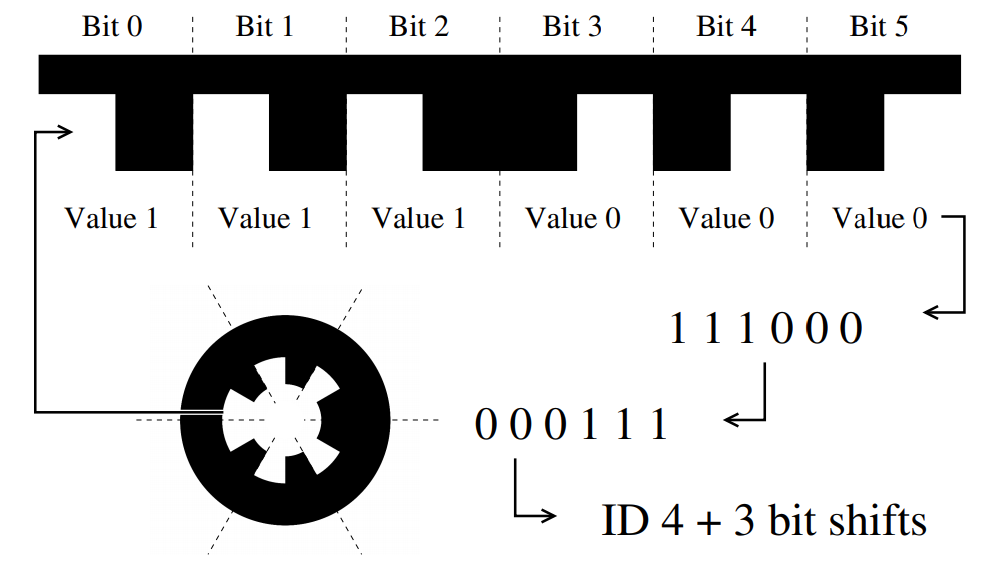
\includegraphics[width=0.5\textwidth]{images/whycode_manchester_explanation.png}
    \caption{The WhyCode marker and ``Necklace'' encoding, from Lightbody et~al.\@.}
    \label{fig:whycode_manchester_explanation}
\end{figure}


As an extension to WhyCon, Lightbody et~al.\@ developed the WhyCode marker in 2017. WhyCode uses the characteristic exterior, circular, black region and interior, circular, white region, but also uses a ``Necklace'' encoding, which is a Manchester encoding of a binary value that is wrapped around the interior white region. This is illustrated in Figure \ref{fig:whycode_manchester_explanation} (from \cite{whycode_paper}). This property of WhyCode markers allows them to break the radial symmetry of WhyCon markers, and also allows them to be distinguished from each other. Some patterns do still have radial symmetry with one another, as some WhyCode IDs have the same shape rotated by some angle. WhyCode markers use essentially the same flood-fill and ellipse-based detection system that WhyCon markers use, but with the added component of a Necklace decoder. The radial asymmetry allows the full spacial pose of the marker to be determined - including the rotational orientation (with some ambiguity based on ID, although this is conceptually able to be overcome). This added benefit makes the marker more appealing than its WhyCon predecessor, while still retaining almost all of the WhyCon computational cheapness. Furthermore, the detection of WhyCode markers is independent from the decoding of the Necklace. This is important because it allows the marker to still be detected in cases where its more intricate encoding is obscured, such as in scenarios of high motion blur or extreme perspective distortion. It also gives the WhyCode marker an edge over the widely-used AprilTag, which must be detected simultaneously with its encoding.




\subsection{PID Controllers}
\label{section:pid_controllers}
The most common form of feedback process controller is the \gls{PID} controller \cite{pid_design}, and indeed these are the most common feedback controllers used in the ArduPilot software. Given a system with a variable to be controlled, an actuator to provide control effort in order to change the variable, and a sensor to read the state of the controlled variable, a PID controller can produce a smooth and predictable change in the state of the controlled variable, causing it to approach and arrive at a set point. A scalar ($k_p, k_i,$ or $k_d$) controls the influence of each of the controller components (proportional, integral, or derivative, respectively) on the control effort. The effect of the proportional component is to apply a control effort which is proportional to the system's error - that is, the difference between the set point and the current state. This causes the state to approach the set point. The effect of the derivative component is to apply a dampening to the control effort which is proportional to the derivative of the error, in order to slow the state's approach to the set point. The effect of the integral component is to apply a control effort which is proportional to the integral of the error, the benefit of which is to remove persistent, steady state errors which must be identified over time and which are therefore not identifiable by the instantaneous readings of the error or its derivative.

The values of the gains must be tuned for each system to which a PID controller will be applied. Some methods exist to analyze systems in order to determine effective gains \cite{pid_design}, however it is also possible to tune the gains manually with some experience. Aside from the gains, it is also necessary to set some other parameters, such as the minimum control effort, the maximum control effort, and the integral windup limit. The minimum and maximum control effort values provide a means of protecting the actuator or system from excessive control forces which may go beyond physical or process constraints. The integral windup limit sets the maximum effect that the integral component may have on the control effort, motivated by the fact that the integral component can easily cause saturation and unstable system response. PID controller tuning is a solved problem and is therefore not described in great detail in this project. \cite{pid_control} and \cite{pid_design} provide guidelines for this, such as the Ziegler-Nichols method.

\subsection{Quaternions}
\label{subsection:quaternions}

Quaternions offer a reliable means of representing rotations in 3-dimensional space. The calculations required to manipulate them are more computationally efficient than matrix operations. Quaternions also do not suffer from the potential ambiguity inherent in representing rotations with 3-dimensional vectors storing values for pitch, roll, and yaw. Pitch, roll, and yaw (rotations in the transverse axis, longitudinal axis, and normal axis, respectively) are visualized in Figure \ref{fig:pitch_roll_yaw}, from \cite{pitch_roll_yaw_dji_source}. These 3-dimensional vectors suffer from loss of information if 2 of the rotational axes become aligned (gimbal lock), and from not providing a single, unique representation for each possible normalized rotation. For these reasons, quaternions are the default data object used to describe rotations in robotics and avionics. A detailed mathematical examination of quaternions is beyond the scope of this project. However, the main ideas behind using quaternions to represent rotation are that they can efficiently be composed with one another, and they represent rotation unambiguously. Mathematically rigorous definitions and explanations of the operations that are relevant to quaternions, as well as the history therein, can be found in \cite{quaternions_reference}.

\begin{figure}
    \centering
    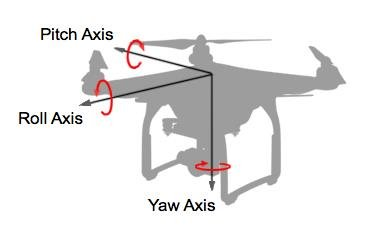
\includegraphics[width=0.35\textwidth]{images/pitch_roll_yaw_dji.png}
    \caption{Visualization of pitch, roll, and yaw.}
    \label{fig:pitch_roll_yaw}
\end{figure}

% Quaternions, as the name suggests, are made up of 4 components. A quaternion $q_1$ is defined in Equation \ref{equation:q_1}:
%     \begin{equation}
%         q_1 = w_1 + x_1i + y_1j + z_2k
%         \label{equation:q_1}
%     \end{equation}
% where $w_1,x_1,y_1,z_1 \in \mathbb{R}$ and $i,j,k$ are orthogonal unit vectors representing typical rotational axes $x,y,z$.  satisfying Equation \ref{equation:quaternion_complex_numbers}.
%     \begin{equation}
%         i^2 = j^2 = k^2 = ijk = -1
%         \label{equation:quaternion_complex_numbers}
%     \end{equation}

% \noindent
% {\color{red} The scalars $x_1,y_1,z_1$ represent the magnitudes of the angles of rotation $\theta_x, \theta_y, \theta_z$ about the axes $x,y,z$ respectively. } Let $\theta$ represent the rotation of $q_1$ about its axis defined by $x_1,y_1,z_1$, then $w$ is defined as in Equation \ref{equation:quaternion_w}:
% \begin{equation}
%     w = \cos \left( {\frac{\theta}{2}} \right)
%     \label{equation:quaternion_w}
% \end{equation}

% \noindent
% Let a second quaternion $q_2$ is defined as in Equation \ref{equation:q2}, again with $w,x,y,z \in \mathbb{R}$, and $i,j,k$ represent the same values as in Equation \ref{equation:q_1}:
% \begin{equation}
%     q_2 = w_2 + x_2i + y_2j + z_2k
%     \label{equation:q2}
% \end{equation}

% \noindent
% Then, in order to ``add'' the rotation described by $q_2$ to the rotation described by $q_1$, the quaternions are \textit{multiplied} using the Hamilton product, as in Equation \ref{equation:quaternion_multiplication}:
% \begin{equation}
%     q_3 = \left( w_2 + x_2i + y_2j + z_2k \right) \left( w_1 + x_1i + y_1j + z_2k \right)
%     \label{equation:quaternion_multiplication}
% \end{equation}

% \noindent
% The resulting quaternion $q_3$ is then equivalent to rotating by $q_1$ and then by $q_2$. In order to ``subtract'' rotations, the inverse of a quaternion is with respect to the Hamilton product is used, as in equation \ref{equation:quaternion_inverse}:
% \begin{equation}
%     q_2^{-1} = \dfrac{1}{w_2^2 + x_2^2 + y_2^2 + z_2^2}\left(w_2 - x_2i - y_2j - z_2k\right)
%     \label{equation:quaternion_inverse}
% \end{equation}

% \noindent
% The result of rotating first by $q_1$ and then by the inverse of $q_2$ can be found by taking the Hamilton product of $q_1$ and $q_2^{-1}$, similarly to Equation \ref{equation:quaternion_multiplication}.

The Transform 2 library (\texttt{tf2}) provides implementations of these data structures and the relevant operations within the ROS infrastructure. The Geometry Messages library (\texttt{geometry\_msgs}) provides message definitions for efficiently representing quaternions in message passing. This project employs these libraries instead of re-inventing the wheel in this area.

\subsection{Robot Operating System}
\label{subsection_ros}
ROS (Robot Operating System) \cite{ros} is an open source framework for developing modular, flexible, robust robotic software. A large variety of modules, libraries, and conventions are included in the \gls{ROS} umbrella. Functional parts of robotic applications are divided into \gls{ROS} modules and libraries, whose definitions provide lists of dependencies and installation instructions, as well as application code. The \texttt{roscore} node (process) provides a means for additional nodes to communicate using \textit{topics}. Topics can be of any data type - such as Boolean variables, integer variables, float variables, images, custom types, etc. Nodes are launched either independently or using \texttt{.launch} files, which specify pre-launch requirements (such as prerequisite nodes), launch parameters, and which may launch additional nodes. A key benefit to using \gls{ROS} is that there are many existing packages supplying many different functionalities, such as \gls{PID} controllers (see Section \ref{section:pid_controllers}), fiducial marker frameworks (see Section \ref{subsection:fiducial_markers}), drivers for cameras (which provide the camera's image as a topic), and many useful data structures such as quaternions (see Section \ref{subsection:quaternions}), vectors. Another important library is the Transform 2 library (TF2) \cite{tf2}, which provides invaluable support for coordinate system transforms. Using this library, nodes can generate time-stamped representations of the positions and orientations of relevant physical components of the robot. These transforms are tagged by name and organized into a tree, after which point, they can be composed with one another to derive further transformations. This is useful in determining the positions of components on the robot itself, and also objects in space.

\subsection{Gazebo Simulator}
\label{subsection:gazebo}
Gazebo \cite{gazebo} is an open source simulation tool developed for Linux. It provides a 3-dimensional environment and a physics engine which allow users to simulate interaction between objects and the environment. Models and worlds can be defined and edited using \texttt{.sdf} and \texttt{.world} files respectively. These files allow users to specify the defining characteristics of each model, such as collision planes which determine how models can make contact with other models or other components within the environment.  Gazebo provides interfaces for simulated sensors, such as inertial measurement units, cameras, LIDAR units, etc., and these sensors can be included in \texttt{.sdf} files in order to provide the relevant information to the model. Plugins can also be included in both \texttt{.sdf} and \texttt{.world} files in order to provide additional functionality, such as \gls{PID} controllers and simulated wind. Several other open source simulators are also available. However Gazebo's existing, readily-compatible plugins for both ArduPilot and ROS make it a good candidate for this project.

\subsubsection{ArduPilot Gazebo Plugin}
\label{subsection:ardupilot_gazebo}
Some Gazebo models and worlds have been developed to allow ArduPilot to interact with Gazebo. They are included in \cite{ardupilot_gazebo_plugin}. For example, the Iris quadcopter (used in this project) is a small quadcopter fitted with a gimbal. The gimbal is a simple, 2-dimensional gimbal with two ``revolute'' joints - a yaw joint referred to as \texttt{iris\_gimbal\_mount}, and a pitch joint referred to as \texttt{tilt\_joint}. \cite{ardupilot_gazebo_plugin} specifies an \texttt{iris\_ardupilot} world file which includes the Iris quadcopter and defines a planar world with a runway. A Python script \texttt{sim\_vehicle.py} provides an interface between the Iris and an instance of ArduPilot. The script reads the data from the simulated sensors aboard the Iris and provides throttle signals to its motor plugins. The motor plugins provide simulated thrust in order to realize the effects of the control system and animate the drone model. These allow the drone system to accurately simulate the behavior of the drone as it is controlled by ArduPilot.

\subsubsection{Integration of ArduPilot, Ground Control Stations, and Gazebo}
\label{subsection:gcs}


ArduPilot can fully interact with and control the Iris quadcopter in Gazebo. The Iris quadcopter model is, as well as several others, specifically set up to mimic the mechanics of an actual quadcopter, and ArduPilot controls the thrust values applied to the motor mounts of the quadcopter. As in a real life scenario, this is the only means of controlling the attitude, velocity, and acceleration of the drone. An instance of ArduPilot can be launched in order to interact specifically with the Iris within Gazebo using the following command: \texttt{sim\_vehicle.py ArduCopter -f gazebo-iris}. This launches the ``copter'' version of ArduPilot which is further configured using the \texttt{gazebo-iris} configuration file. ArduPilot further opens \gls{UDP} ports in order to communicate with \gls{GCS} instances using the MAVlink communication protocol. In this project, care has been taken to leave both the ArduPilot software and MAVLink protocol unmodified, such that it may be applied to existing drone systems without deep modification.

Several different \gls{GCS} programs are also available open-source. These typically offer a GUI for visualization and temporal tracking of a vehicle's position in a map, forms for adjusting various parameters, displays for sensor values, and, importantly, a concise, GUI-based method of sending MAVLink commands to the vehicle. The QGroundControl software \cite{qgroundcontrol} is the software chosen for interacting with the simulation in this project purely because of its simplicity of installation. Alternatives would also work, but the particular choice of \gls{GCS} software is unimportant.

\section{Related Work}
\label{section:related_work}
Wynn \cite{wynn} has developed a method for landing on a moving platform using fiducial markers to track the landing platform, with the initial aid of GPS. A larger marker allows recognition of the landing platform from far distances. A smaller marker of the same form is embedded inside the larger marker to allow for identification at close distances. After the landing platform is localized, different control states direct the drone's approach towards the marker - first causing the drone to approach quickly in the x and y dimensions, while maintaining a sufficient altitude above the marker (in the z dimension), and then gradually lowering to a small distance above the marker. At this point, the drone commits to a landing and lowers itself until detecting a successful landing, since the proximity of the camera to the landing pad means that the marker is no longer fully contained within the field of view of the camera, and thus can no longer be tracked. Other control states include switching from \textit{patrol mode} to \textit{tracking mode} once the relevant marker has been detected continuously for a small amount of time, and aborting a landing if the marker has not been detected for 2 seconds continuously. This method also takes into account the swaying of the landing platform itself, which is mounted on a barge.

Borowczyk et~al.\@ \cite{high_velocity_landing} have implemented a system allowing a DJI Matrice to land on a golf cart using \gls{GPS} with wirelessly transmitted position. The drone uses a \gls{PN} system for initial approach. This initial approach is carried out at a fixed altitude and a gimbal-mounted camera is used for initial detection of a fiducial marker mounted to the landing platform. A fixed, downward-facing camera then detects the visual fiducial marker and a \gls{PID} controller manages close-range approach. A constant descent velocity is set during the final phase of landing. This method allows for successful landing on a platform moving at speeds of up to 50 km/h. Recommended future work includes using multiple fiducial markers of different sizes to identify the landing platform, as well as a single gimbal-mounted camera instead of the dual camera setup.

Falanga et~al.\@ \cite{vision_based_x_platform} outline a method for landing a quadrotor running the PX4 autopilot software on a moving platform indoors. The landing platform is fitted with a specific marker made up of a cross and a circle. The drone uses 2 cameras, the first mounted straight down from the drone, and the second mounted at a 45\degree angle down and towards the front of the drone. The images from these cameras are used to solve a \gls{PnP} problem which finds the relative pose of the landing platform's marker. A distance sensor helps to scale the vision-based pose estimation. The onboard computer determines optimal approach trajectories using this information. A Kalman filter makes the process robust to missed detections and helps to determine the velocity of the landing platform. Successful landings were reported with the landing platform moving up to 1.2 m/s.

Wubben et~al.\@ \cite{accurate_landing_UAV_ground_pattern} use the typical setup of a hexacopter drone with a single camera in a fixed, downward facing orientation to identify a landing platform via 2 ArUco markers. A Pixhawk controls the drone using ArduPilot, and a Raspberry Pi handles image processing and fiducial identification. The method reports successful and accurate landings, but also occasional failures due to visual loss of the landing platform. This visual loss was caused by sudden gusts of wind which pushed the drone away from the landing platform and out of the fixed camera's field of view.

Pluckter et~al.\@ \cite{drone_landing_unstructured_environments} have developed a method for precisely landing a drone in an \textit{unstructured} environment, which is to say an environment that has not been significantly artificially marked. On takeoff, the drone visually captures key points of interest in its environment. It then performs its mission and returns to a location above its takeoff location using \gls{GPS}. Subsequent visual analysis of the surroundings and comparison of this information with the similar information captured at takeoff allow the drone to localize itself. This process is continued throughout the entire landing.

Polvara et~al.\@ \cite{drq_landing} introduce a method of training and testing \gls{DQN} for landing drones in a simulated environment with simple outputs (left, right, forward, back, land), feeding the networks low-resolution images as input. Multiple networks were trained for specialized tasks, such as policy control, approach, and descent. The method performed with only slightly less accuracy than the conventional vision-based methods which use fiducial markers. However, the caveat is that the conventional methods can fail when the fiducial marker cannot be detected, whereas the method presented by Polvara et al still achieved a relatively high success rate.

Patrick Irmisch \cite{apriltag_whycon_comparison}, in his master thesis at the Technical University of Berlin, compared distance estimation of AprilTags and WhyCon markers (Shown in Figure \ref{fig:fiducial_markers}) using both monocular and stereo computer vision algorithms. This was done in an effort to use computer vision as a way to estimate the distance between two trains as one approached the other for coupling. The markers were printed such that they occupied the same area, and multiple tests were carried out to determine the error in distance estimation when viewed from angles of 0\degree, 30\degree, and 60\degree. The stereo vision methods were tested using multiple matching algorithms, including the \gls{PnP}, and \gls{SGM}. The distance from the camera to the markers was estimated by these methods when the true distance varied between 10 and 80 meters. Distance estimation (that is, distance on the z-axis) is arguably the hardest part of a pose to estimate, since it involves composite measurements and calculations. Positions on the x-axis and y-axis can be easily determined through simple pixel analysis, and distortion can be used to measure the angle between the camera and the fiducial marker in each axis when the form of the fiducial marker is known. However, z-axis distance estimation is influenced by the distance itself, since at longer distances the fiducial marker occupies less pixels, meaning that the resolution between different distances is obscured. All of the fiducial markers show some robustness in their ability to be detected even when viewed from a far distance or from an angle. The real-world experiment showed that the distance from the camera to a WhyCon marker could be estimated with less error than that of an AprilTag marker. The WhyCon marker can also be detected from farther away, whereas the AprilTag marker was not detectable at a distance of 40 meters. The WhyCon marker was detected at a distance of 40 meters even at a viewing angle of 60\degree. Simulations showed more robust detection of both AprilTag and WhyCon markers, but this is not particularly important in the context of the real-world. Uncertainty in distance estimation actually increased in the tested stereo vision methods, likely owing to the doubled uncertainty in camera calibration parameters and camera orientation. However, a small decrease in distance estimation error was attained when combining both monocular and stereo methods. Ultimately, the results imply that a single WhyCon marker is the most suitable for relative position estimation between vehicles. Irmisch goes on to recommend that WhyCon markers be used with a stereo vision setup, with \gls{SGM} as the detection algorithm.


Guo et~al.\@ \cite{monocular_pose_estimation} illustrate a monocular pose estimation system which is used to estimate the position of a multicopter indoors and without GPS. The given scenario involves a drone determining its position above a mat on the floor with several April Tag markers printed on it, each with a different identifier. The single camera is fixed to point facing straight down from the drone. Their system uses a set of translation and rotation matrices to calculate the position of the drone in the indoor flying space. The translation and rotation matrices from the camera to the tag are computed when the detection algorithm for the AprilTag identifier determines the pose of the AprilTag with respect to the camera. These are converted from pixel distances to real-world lengths using the intrinsic parameters of the camera. After these are determined, the position $P_M$ of the drone on the map can be calculated directly because the rest of the values are constant. The accurate position of the drone is then derived from $P_M$ using a Kalman filter to reduce noise. Detailed results are not presented, but the drone is able to fly from tag to tag following a planned path with high accuracy, estimating its position only from identifying and determining the relative position of April Tag markers in the map.

% \begin{equation}
% P_M = T_{T_k}^M + R_C^{T_k}\left(P_C + T_B^C\right) + T_C^{T_k}
% \end{equation}

% where
% \begin{itemize}
%     \item $P_M$ is the position of the drone on the map,
%     \item $T_{T_k}^M$ is the fixed translation matrix from the $k^{th}$ tag to the map,
%     \item $R_C^{T_k}$ is the rotation matrix from the camera to the $k^{th}$ tag,
%     \item $P_C$ is the position of the camera, determined by identifying the $k^{th}$ tag,
%     \item $T_B^C$ is the fixed position of the camera with respect to the drone (it is mounted slightly forward, not in the center), and
%     \item $T_C^{T_k}$ is the translation matrix from the camera to the $k^{th}$ tag.
% \end{itemize}



\section{Structure of this Thesis}
The motivated design and data flow of the gimbal and landing controllers is presented in Chapter 1, along with the supporting software infrastructure, and conditions of the simulation environment. Quantitative analyses of the performances of these systems within the simulator are presented in Chapter 3. Guidelines for the migration of this system from the simulator to a physical drone are presented in Chapter 4.

\chapter{Methods}
\section{Landing System Requirements and Design Overview}
\label{section:requirements}
The landing controller must be robust to the positional noise apparent in normal GPS modules, which can cause mishaps during landing, meaning it must have a positional accuracy on the order of about 0.2 meters when targeting a landing platform with a diameter of 1 meter. It must also allow for landing on both stationary and moving landing platforms. To this end, the landing controller does not use GPS as its main navigational source, but instead uses fiducial markers as mentioned in Section \ref{subsection:fiducial_markers}, to estimate its position with respect to the landing platform. In order to land safely, the landing controller must have a way to identify and stop a failed landing, which could be caused by erratic landing platform movement, drift due to wind, obfuscation of the landing platform's fiducial markers, etc. In order to accomplish this, a descent region is generated, as shown in Figure \ref{fig:descent_region}. The radius of this region increases exponentially in the altitude of the drone above the landing pad. Outside of this region, the drone is not allowed to descend. This gives the drone time to correct its horizontal position and maintain a safe descent. This is outlined in Section \ref{subsection:control_policy}.

The landing platform must be recognizable under a wide variety of conditions. A gimbal-mounted camera increases the range in which the landing platform can be identified by the camera. This requires the addition of a gimbal controller which aims the camera for the duration of the landing, explained in Section \ref{section:gimbal_controller}. A large WhyCon marker allows for easy recognition of the landing platform from long distances, while a smaller April Tag marker provides continuous pose estimation throughout the final descent, when the WhyCon marker is not entirely visible in the camera's field of view.

The landing controller and gimbal controller must be easy to integrate into existing drone systems. As mentioned in Section \ref{subsection:ardupilot}, the chosen autopilot software is ArduPilot, which uses the MAVLink communication protocol. To allow the proposed landing system to be easily integrated into existing drone systems, the ArduPilot code and MAVLink dialects are not edited. The landing controller and gimbal controller are developed as ROS modules which can be run on a companion board, interfacing with ArduPilot for control. On more advanced flight controllers, such as Navio2-enabled Raspberry Pis (which have full operating systems), these ROS modules can be run on the same board as the ArduPilot software, as system services. In order to abstract from primitive motor throttle commands and specific drone body types, the landing controller controls the drone using only high-level velocity set points. This leaves the low-level motor control to ArduPilot itself. The hardware tool set is also kept simple (just a gimbal-mounted camera and a companion board) for this requirement.

\section{System Evaluation through Simulation}
Simulation is a fast and cheap way of testing drone control algorithms, as it cuts out the overhead of physical components and the risk of fatal, expensive crashes. However, it does have the added overhead of adapting a specific model to a specific simulation environment, which can be a daunting task. Furthermore, the results of the simulation - particularly the model physics - likely will not translate directly to the real world. Ultimately this means that simulation can be aptly used for testing the landing system at a high level, but that transitioning to real world flight will involve incremental re-testing. In other words, simulation is only a good first step.


\subsection{Setup and Tools}
\label{subsection:setup_and_tools}

The Gazebo 9 simulator and the ArduPilot-compatible Iris quadcopter drone model (and included gimbal model) are provided in the open source community, as discussed in Section \ref{subsection:gazebo} and Section \ref{subsection:ardupilot_gazebo} respectively. These systems have existing integration with each other and with \gls{ROS}, making them an ideal combination of tools for this project. The development of a new drone model for simulation is beyond the scope of this project. However, even though there is a slight discrepancy in that the simulation model is a quadcopter and the destination platform is a hexacopter, the proposed landing system is abstracted enough to overcome this difference. All of the commands sent by the landing controller are target velocities rather than primitive controls such as throttle signals to specific motors. The frame (quadcopter or hexacopter) can be manually set in the ArduPilot on-board firmware.

% The open-source autopilot softwares ArduPilot and PX4 both have open source drone models available for use in an open source simulator called Gazebo. The model that has been used in this simulation is Gazebo's Iris quadcopter, which has plugins for both ArduPilot and PX4. 

\subsubsection{Simulation World}

\begin{figure}[ht]
    \centering
    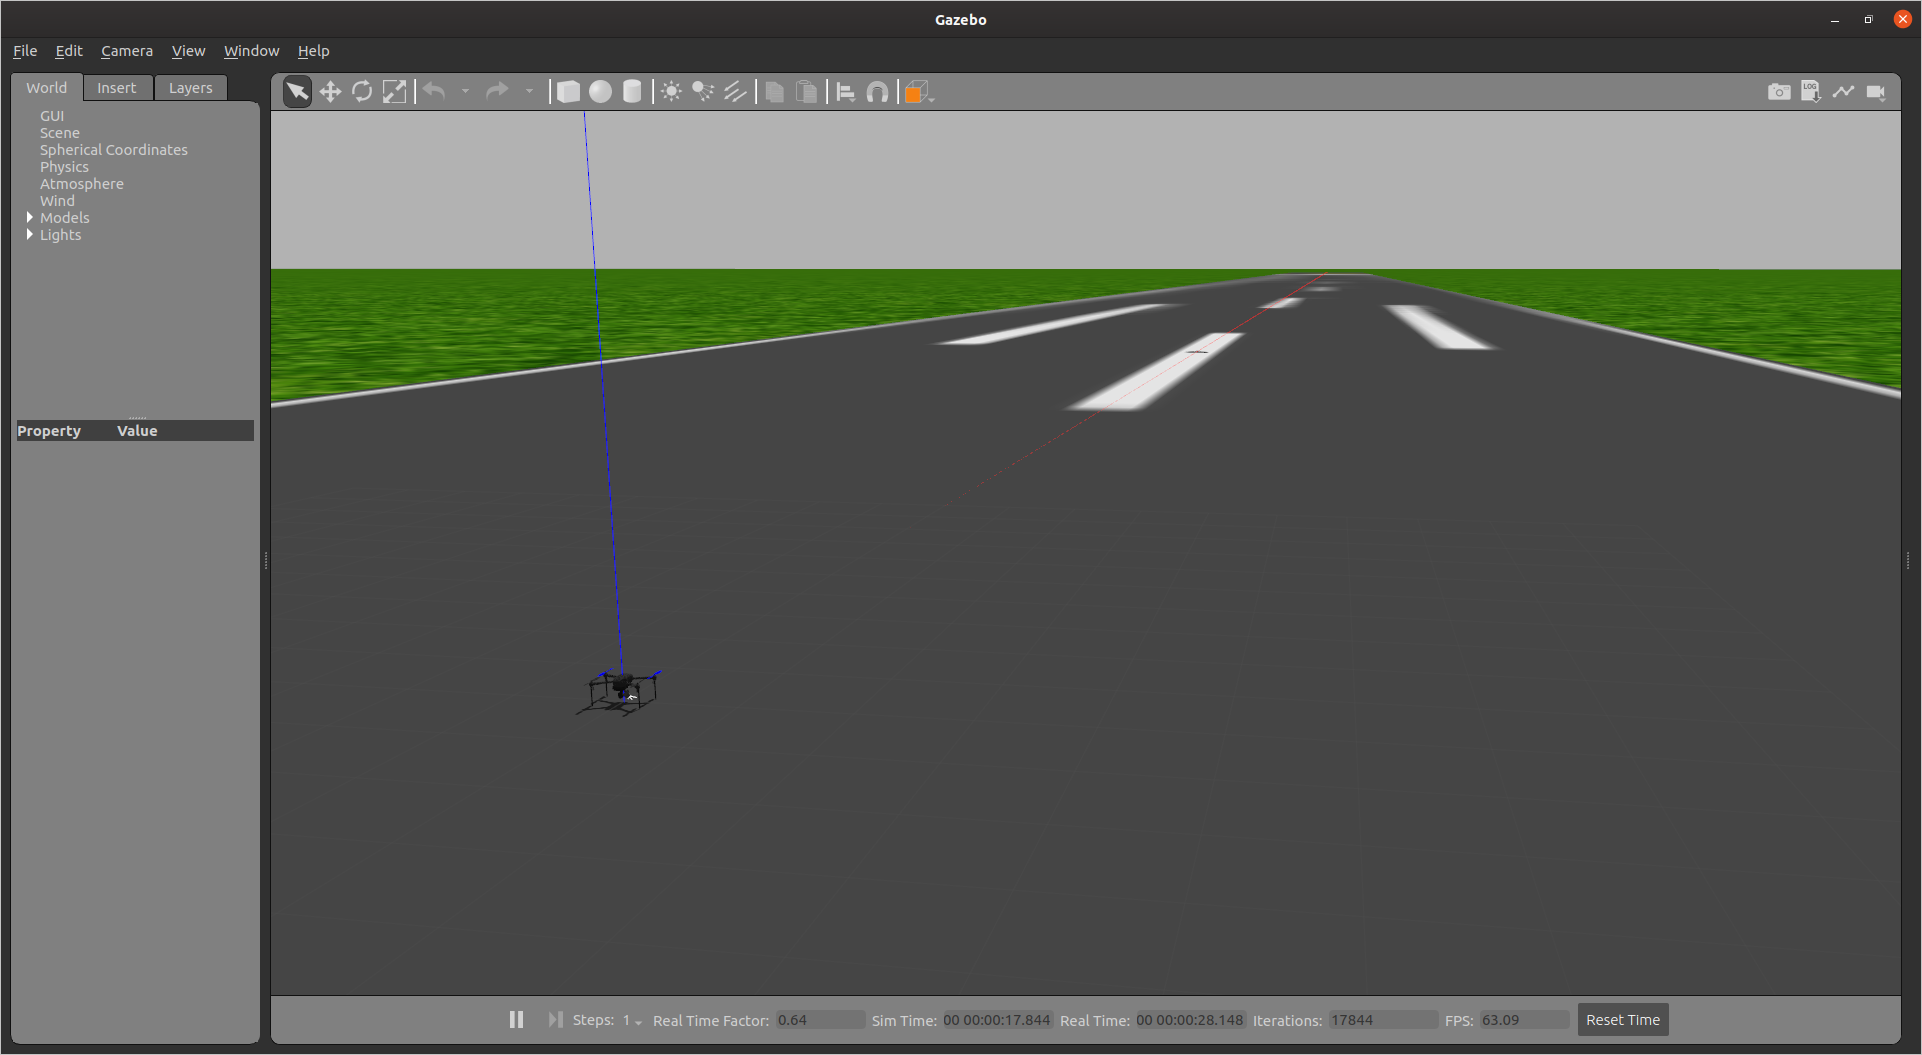
\includegraphics[width=0.6\textwidth]{images/gazebo.png}
    \caption{Gazebo GUI with the Iris quadcopter model.}
    \label{fig:gazebo}
\end{figure}

% \subsubsection{Simulation World}

The simulation uses Gazebo 9 as its base, as shown in Figure \ref{fig:gazebo}. However, in order to interface with ROS, Gazebo is launched through ROS itself, with the following command: \texttt{roslaunch gazebo\_ros sandbox.launch}, where \texttt{sandbox.launch} opens a ``sandbox'' world created for the purpose of experimentation. It is an edited version of the \texttt{iris\_ardupilot.world} which includes a landing platform made from fiducial markers, explained in Section \ref{subsection:landing_pad_design}. It includes the specification for the Iris quadcopter, along with an edited version of the Iris' gimbal. The edited version of the gimbal adds a weightless, simulated camera sensor that provides its detected image to an instance of ROS as a ROS topic. This particular sensor is available from the \texttt{gazebo\_ros\_pkgs} repository. This is necessary because the included gimbal model does not include a camera sensor. The typical paradigm for adding a simulated sensor (such as this camera) to a Gazebo model involves adding not only the sensor itself, but also a ``link'' component which contains the sensor and inherently has mass. This paradigm was not followed here because the addition of such a link with any mass, including, zero and near-zero mass values such as $10^{-10}$ kg, caused prohibitively unstable in-flight behavior of this particular model. The weightless camera sensor was thus attached simply to the gimbal's \texttt{tilt\_link}. The definitions for the edited models and worlds are available at \cite{edited_ardupilot_gazebo}.
% \footnote{The working specifications for the models and world described above are available in \href{https://github.com/uzgit/ardupilot_gazebo}{this github repository}, which is a forked version of \href{https://github.com/SwiftGust/ardupilot_gazebo}{this repository}, which is itself a forked version of the original \href{https://github.com/khancyr/ardupilot_gazebo}{\texttt{ardupilot\_gazebo} repository}.} 
The simulated camera view is shown in Figure \ref{fig:gazebo_camera}. This visualization allows developers to have an intuitive sense of the drone's field of view, which is especially important in a situation like this, when the camera rotates on a gimbal. 

\begin{figure}
    \centering
    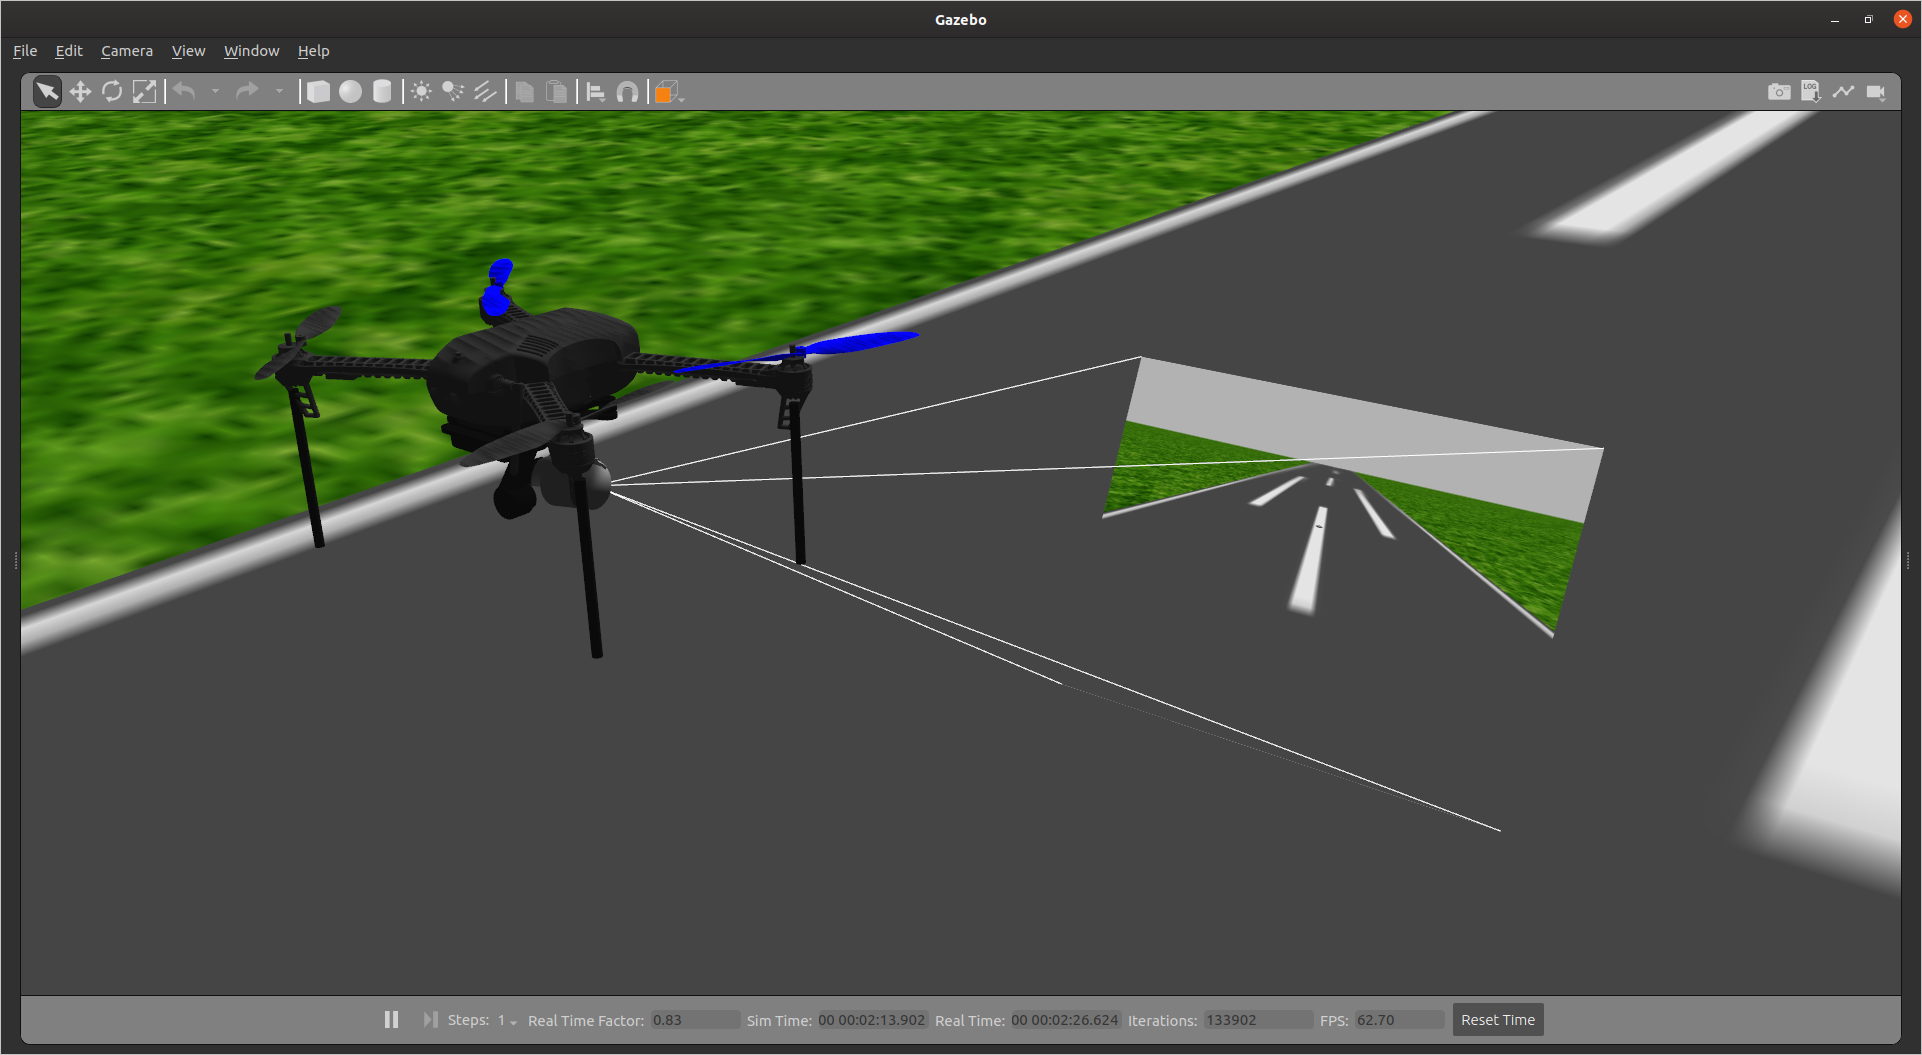
\includegraphics[width=0.6\textwidth]{images/gazebo_camera.png}
    \caption{The view of the drone's camera in Gazebo.}
    \label{fig:gazebo_camera}
\end{figure}

\subsubsection{\gls{GCS} Software}

The chosen \gls{GCS} software for this project, as mentioned in Section \ref{subsection:gcs}, is QGroundControl, which is depicted in Figure \ref{fig:qgroundcontrol}. There are several \gls{GCS} alternatives available open source. This particular one was chosen purely because of its ease of installation, but this choice is not important to the outcome of this project. It is only necessary to have some \gls{GCS} software, as it provides easy manual control of the drone in the absence of a conventional radio remote controller during simulation. This is important particularly in the early stages of testing, to perform ad hoc testing and to determine strategies for more formal, automated testing as will be described in Chapter \ref{chapter:simulation_results}.

\begin{figure}[ht]
    \centering
    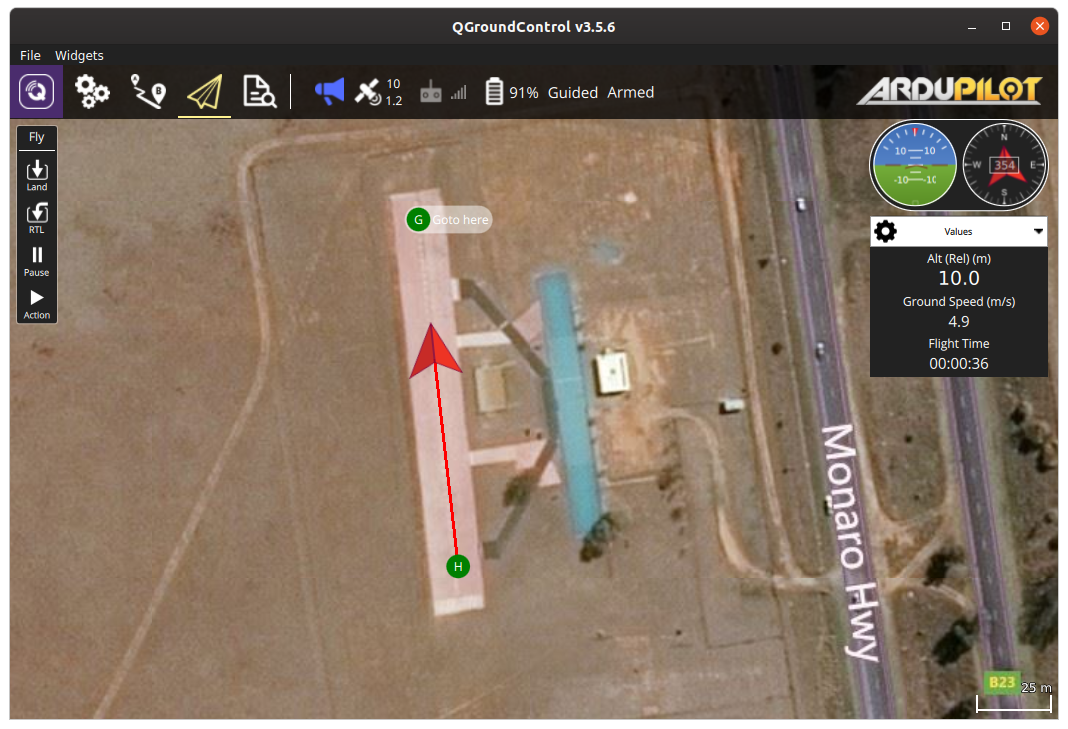
\includegraphics[width=0.6\textwidth]{images/qgroundcontrol.png}
    \caption{The QGroundControl software.}
    \label{fig:qgroundcontrol}
\end{figure}

% The landing area, shown in Figure \ref{fig:landing_pad} is comprised of two separate markers. The large circular WhyCon marker is used for long-range identification of the landing pad, as its simpler design and lack of inherent identifier make it easier to recognize from farther away. An April Tag marker is positioned in front of the landing pad, so that it will be visible throughout the drone's entire descent, albeit from a sharp angle of deflection. The April Tag's distinct identifier means that its unambiguous orientation can be determined reliably, even at sharp angles of deflection. This means that, once the large WhyCon marker has eclipsed the camera's field of view, the drone will still have reliable visual localization capabilities with which to estimate its position relative to the landing pad. More information on the theory behind these fiducial markers, as well as empirical comparisons of their performance are outlined in Section \ref{subsection:fiducial_markers}, and in the papers cited therein. Importantly, both of these fiducial systems have open-source ROS modules available, meaning that the development of a fiducial marker was not necessary for this project. The image from the simulated camera is provided as input to both fiducial systems, so that two different estimations of the landing pad's position are available. The dimensions and positions of the markers, and the distortion matrix of the camera are known to the landing system, so that the system can accurately estimate the landing pad's position. The drone targets the center of the WhyCon marker as its point of contact with the landing pad, and the gimbal controller generates a coordinate transform to align the drone with the center of the WhyCon marker using only the April Tag marker, when the WhyCon marker itself is not in view. 

% \begin{figure}
%     \centering
%     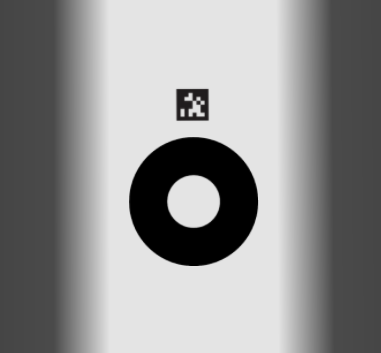
\includegraphics[width=0.6\textwidth]{images/landing_pad.png}
%     \caption{Landing pad design.}
%     \label{fig:landing_pad}
% \end{figure}

\section{Gimbal Controller}
\label{section:gimbal_controller}

\subsection{Overview}

In experiments using drones with a mounted camera, it is typical to see a camera with a fixed mounting angle. This provides simplicity in the estimation of the drone's pose relative to some fiducial marker, but limits the ability of the drone to detect the marker, as the drone itself must be facing the marker in order to detect it in the first place. A key aspect of this project is the development of a method for pose estimation of a drone relative to a fiducial marker using a gimbal-mounted camera for a wider range both of relative pose between the marker and the drone, and a wider range of acceptable behaviors for the drone during landing. This requires a slightly more involved system for coordinate transforms, as well a method for aiming the gimbal at the marker and tracking it over time.

\subsection{Data Flow}

\begin{figure}[ht]
    \centering
    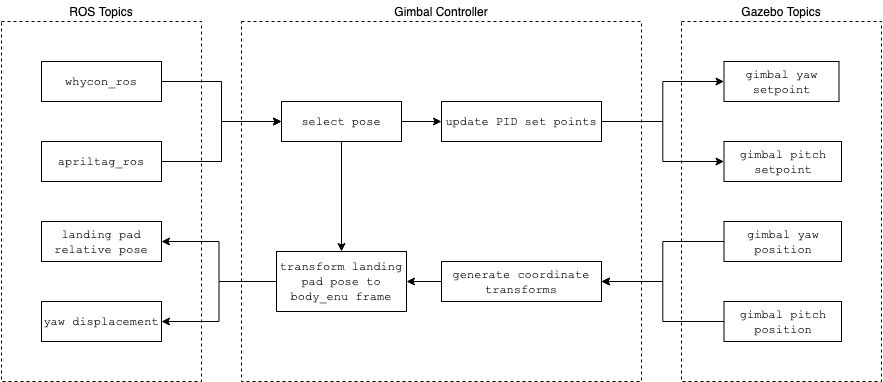
\includegraphics[width=\textwidth]{images/gimbal_controller_diagram.png}
    \caption{Gimbal controller data flow diagram.}
    \label{fig:gimbal_controller_diagram}
\end{figure}

The diagram in Figure \ref{fig:gimbal_controller_diagram} gives a high-level overview of the gimbal controller's functionality. The WhyCon and April Tag modules publish the pose of their possibly identified fiducial markers after analyzing the image from the simulated camera. If either module finds no marker in the image, then that module publishes no pose. If both markers are detected at the same time, only the April Tag marker is selected, and if only a WhyCon marker is detected, then it is used. The gimbal controller then updates the PID set points according to Equation \ref{equation:setpoints} and these are used by the PID controller instances in Gazebo. The gimbal controller subscribes to the true yaw and pitch positions of the gimbal, provided by Gazebo, which are not necessarily equal to the set points. These gimbal yaw and pitch positions provide the necessary information to generate the coordinate transform from the camera frame to the body ``ENU'' (East, North, Up) frame. The landing platform pose is then transformed to the body ENU frame and is published as its own topic. The ``yaw displacement,'' denoting the angle between the north axis of the drone and the north axis of the landing pad, is also published as a topic. 

The typical NWU (North, West, Up) coordinate system of Gazebo is visualized in Figure \ref{fig:nwu_coordinate_system}, with the red axis line pointing to the drone's ``north,'' the green axis line pointing to the drone's ``west,'' and the blue axis line pointing up. This is in contrast to the typical ROS \gls{ENU} coordinate system, in which the axis lines in Figure \ref{fig:nwu_coordinate_system} would be rotated by 90\degree clockwise in the ``up'' axis, so that the red axis points east, the green axis points north, and the blue axis points up. These lines represent the positive directions of their respective axes.

\begin{figure}[ht]
    \centering
    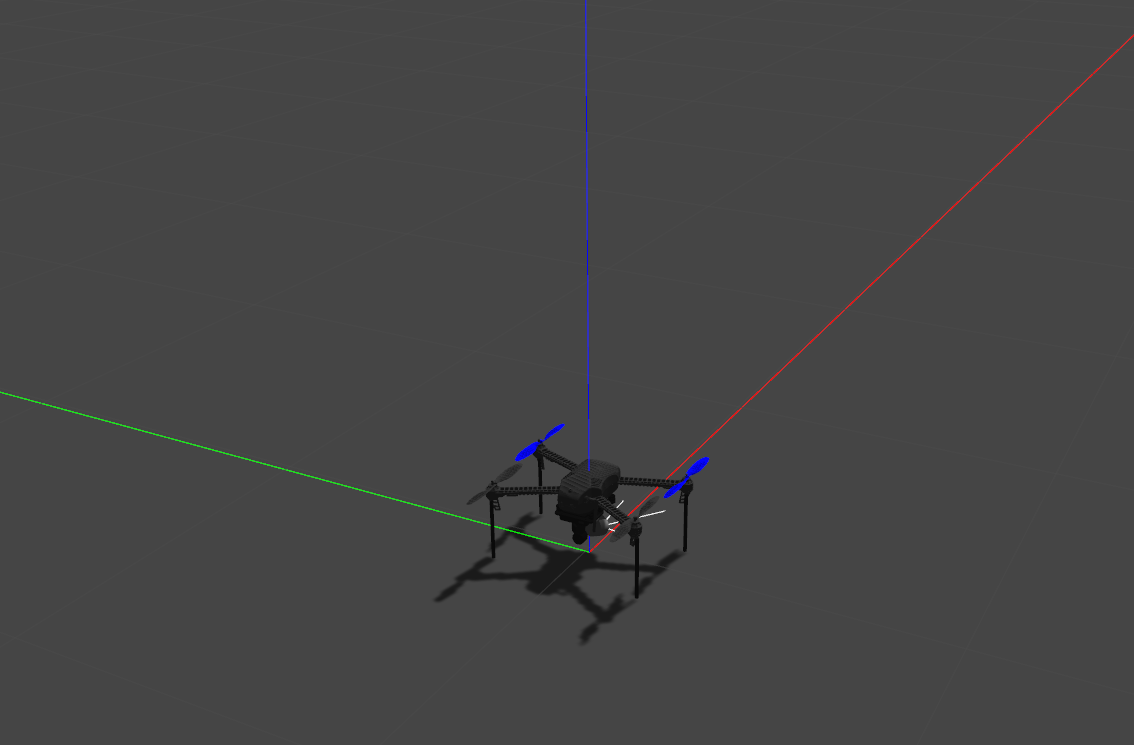
\includegraphics[width=0.6\textwidth]{images/nwu_coordinate_system.png}
    \caption{NWU (North, West, Up) Coordinate System within Gazebo.}
    \label{fig:nwu_coordinate_system}
\end{figure}

\subsection{PID Controllers for Gimbal Control}

\gls{PID} systems (outlined in Section \ref{section:pid_controllers}) provide a natural solution to the problem of aiming the gimbal, with the goal being to keep the marker in the center of the camera's field of view at all times. It would also be natural, therefore, to control the position of the camera based on the pixel positions of the detected fiducial markers. However, both the April Tag and WhyCon systems provide the positions of their markers in the form of a pose (\textit{not} pixel locations) - a specification of the linear translation and spacial orientation from the viewpoint to the marker. These poses are composed of a 3-dimensional vector providing the translation in (simulated) meters, and a quaternion providing the orientation. It is simple to control the position of the camera using the poses of the detected fiducial markers - instead of using pixel locations - in order to avoid additional edits to the already existing code, and also to avoid potentially required specificity to any hardware system (cameras may have different pixel ranges and therefore different centers).

\subsubsection{Gazebo Plugin Implementation for Gimbal Control}

A Gazebo plugin was added to the simulated drone's gimbal provide \gls{PID} control of the orientation of the gimbal and camera. The plugin is defined as a ROS module, is included in the model's definition \texttt{.sdf} file, and its library is loaded by Gazebo at runtime. This plugin subscribes to ``setpoint'' topics that are provided by the \texttt{gimbal\_controller} ROS module. As the gimbal has 2 degrees of freedom (yaw and pitch), 2 corresponding \gls{PID} controllers set the orientation of their respective gimbal axes. The gimbal has artificial limits of $\theta_{yaw} \in \left[ -\frac{\pi}{2}, \frac{\pi}{2} \right]$ and $\theta_{pitch} \in [0, \pi]$ for simplicity. $\theta_{yaw} = 0$ describes a situation where the camera is pointing directly forward (with respect to the drone's local coordinate frame), and $\theta_{yaw}$ increases as the camera rotates clockwise. $\theta_{pitch} = 0$ describes a situation where the camera is pointing forward, directly level to the drone. $\theta_{pitch}$ increases as the camera rotates towards vertical-down. The 2 \gls{PID} controllers are able to control the position of the camera only in these ranges, which helps the system to avoid unnecessary rotations during simulation and also mimics the natural limits of physical systems. The gains of these systems were determined experimentally and will be described in Section \ref{subsection:pid_tuning}. The plugin also publishes the true angles of the gimbal in each dimension as ROS topics for the subsequent calculation of coordinate transforms, explained in Section \ref{subsection:coordinate_system_transforms}.

\subsection{Aiming the Camera}
\label{subsection:aiming_the_camera}

The gimbal controller has callback functions for both WhyCon and April Tag detections, where it updates the set points (target states) of both \gls{PID} controllers. Let $SP_x$ be the set point of the gimbal's yaw axis, and let $SP_y$ be the set point of the gimbal's pitch axis. The yaw and pitch axes of the gimbal can be visualized in Figure \ref{fig:gazebo_camera}, where the yaw of the gimbal is in line with the yaw of the drone ($\theta_{yaw}=0$), and the pitch of the gimbal is slightly less than that of the drone ($\theta_{pitch} > 0$). Then, upon detection of a fiducial marker, the set points are updated as in equation \ref{equation:setpoints}:

\begin{equation}
    \begin{array}{l}
        SP_x = SP_x - k \frac{x}{z} \\
        SP_y = SP_y + k \frac{y}{z}
    \end{array}
    \label{equation:setpoints}
\end{equation}

where $k$ is an experimentally determined scalar, and $x,y,z$ are the linear components of the marker's pose in the west, down, and north axes of the camera respectively. The callback functions \textit{increment} the set points instead of calculating them directly. The difference in the sign of the increment occurs because of the specific nature of Gazebo's axis conventions. This particular aspect would require special attention and verification when transitioning to a real world environment. The increment is scaled inversely to $z$ in order to ensure that the system works over a range of distances. 

\subsection{Landing Pad Design and Prioritization of Fiducial Marker Detections}
\label{subsection:landing_pad_design}

\begin{figure}[ht]
    \centering
    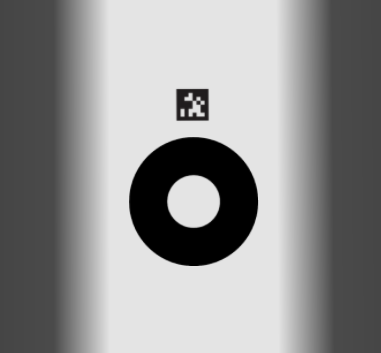
\includegraphics[width=0.6\textwidth]{images/landing_pad.png}
    \caption{Landing pad design.}
    \label{fig:landing_pad}
\end{figure}

As shown in Figure \ref{fig:landing_pad}, the landing pad is made up of two markers. The system recognizes the larger (1 meter in diameter), more easily identifiable WhyCon marker before it recognizes the April Tag marker (with side length 0.3125 meters). However, since the April Tag marker is used for final descent at close range, the gimbal controller prioritizes the April Tag marker over the WhyCon marker. So in the case that both markers are visible, the gimbal controller aims the camera at the April Tag marker. If the April Tag marker becomes obstructed, the gimbal controller then aims the camera at the WhyCon marker again. This prioritization is illustrated in Figure \ref{subfig:whycon_detection_only} through \ref{subfig:centered_april_tag_detection}. In the detection windows, detected WhyCon markers are highlighted, and detected April Tag markers have their IDs printed above the marker itself. The fact that the April Tag marker is flat on the landing pad's plane does mean that, at a low altitude, it will be somewhat difficult to recognize the April Tag's pose. However, this is a challenge to overcome anyway, as it keeps the landing pad simple and completely flat (and therefore free of obstructions). The center of the April Tag marker is positioned 0.75 meters north of the center of the WhyCon marker. This allows for the marker to be adequately close to the drone during final descent that it can always be easily recognized. However it also means that the April Tag marker is adequately displaced from the camera to always be in the camera's field of view. This distance is likely to be adjusted in real world experiments. The original design for the landing platform included only a single WhyCode marker, but this was abandoned for reasons that will be discussed in Section \ref{subsection:whycode_trials}.

% \begin{figure}
%     \centering
%     \subfloat[WhyCon detection only.\label{subfloat:whycon_only}]{{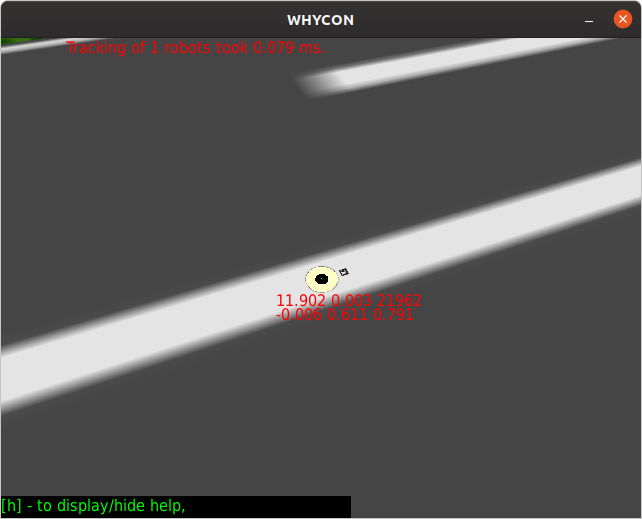
\includegraphics[width=0.45\textwidth]{images/whycon_detection_only.png} }}
%     \hfill
%     \subfloat[No April Tag detection.\label{subfloat:no_apriltag}]{{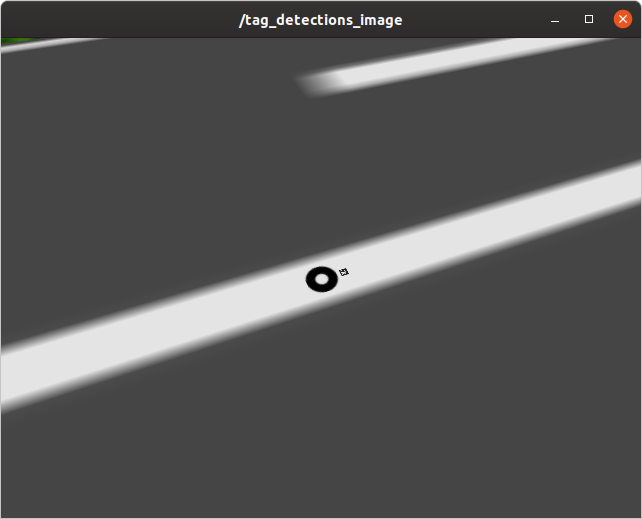
\includegraphics[width=0.45\textwidth]{images/no_apriltag.png} }}\\
%     \subfloat[Off-center WhyCon detection.\label{subfloat:off_center_whycon}]{{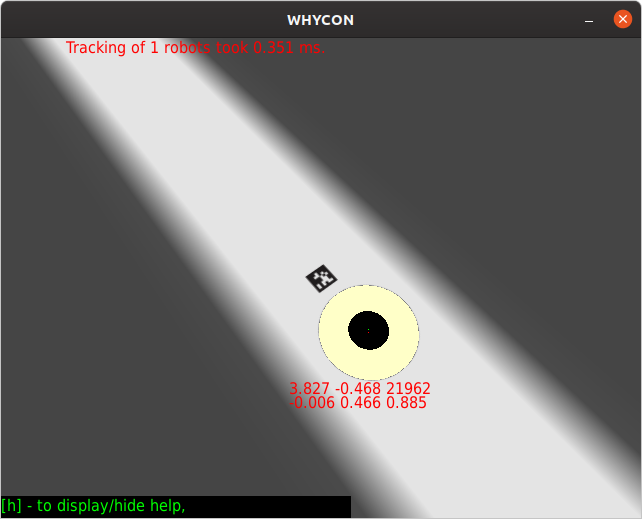
\includegraphics[width=0.45\textwidth]{images/whycon_off_center.png} }}
%     \hfill
%     \subfloat[Centered April Tag detection.\label{subfloat:apriltag_detection}]{{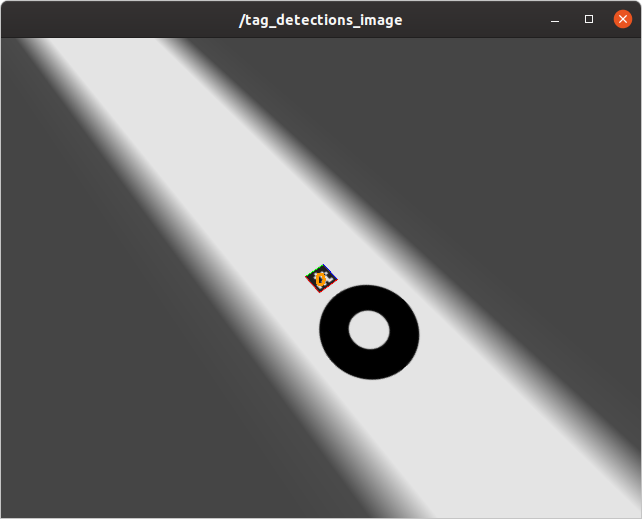
\includegraphics[width=0.45\textwidth]{images/apriltag_detection.png} }}
% \end{figure}

% [height=6.5cm]

\begin{figure}
     \centering
     \begin{subfigure}[b]{0.49\textwidth}
         \centering
         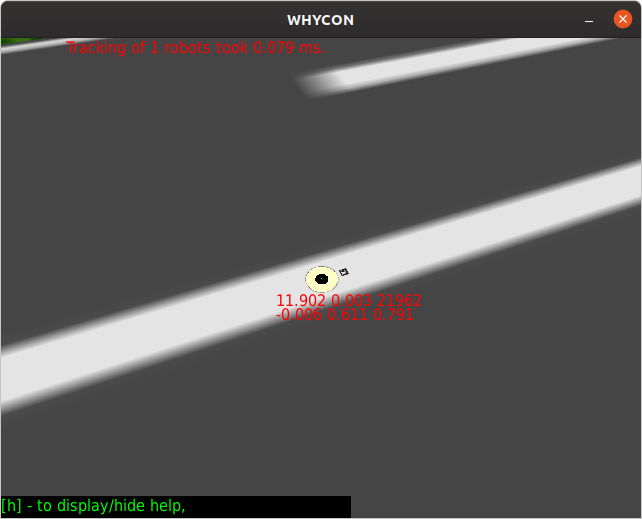
\includegraphics[width=\textwidth]{images/whycon_detection_only.png}
         \caption{WhyCon detection only.}
         \label{subfig:whycon_detection_only}
     \end{subfigure}
     \hfill
     \begin{subfigure}[b]{0.49\textwidth}
         \centering
         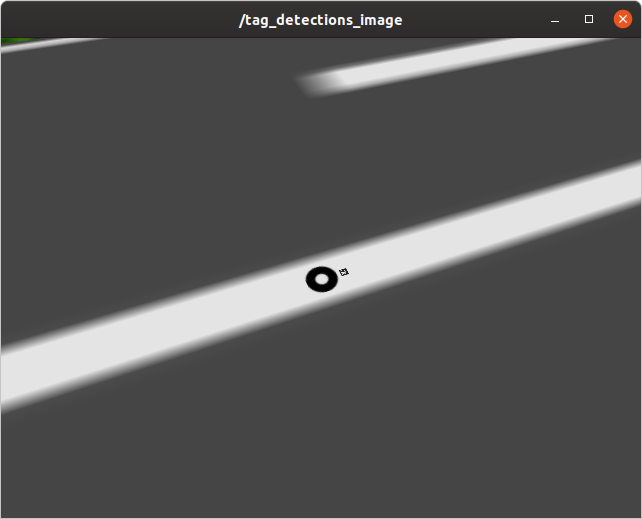
\includegraphics[width=\textwidth]{images/no_apriltag.png}
         \caption{No April Tag detection.}
         \label{subfig:no_apriltag_detection}
     \end{subfigure}
     \begin{subfigure}[b]{0.49\textwidth}
         \centering
         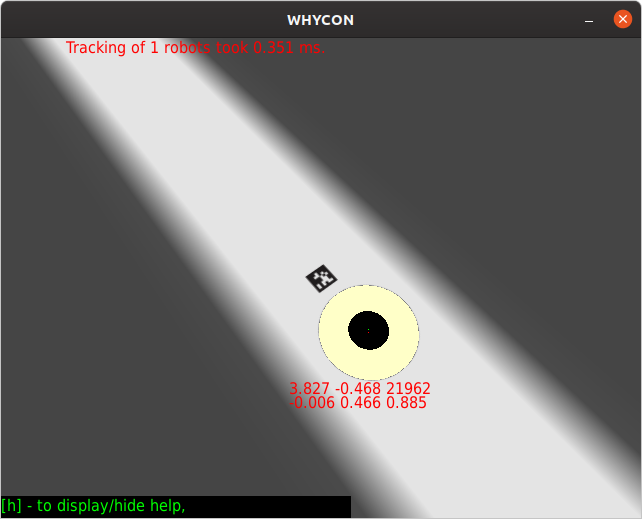
\includegraphics[width=\textwidth]{images/whycon_off_center.png}
         \caption{Off-center WhyCon detection.}
         \label{subfig:off_center_whycon_detection}
     \end{subfigure}
     \hfill
     \begin{subfigure}[b]{0.49\textwidth}
         \centering
         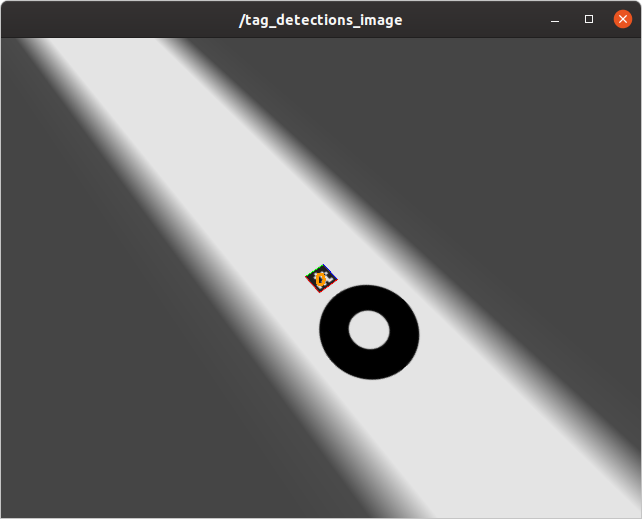
\includegraphics[width=\textwidth]{images/apriltag_detection.png}
         \caption{Centered April Tag with ID ``0'' overlayed.}
         \label{subfig:centered_april_tag_detection}
     \end{subfigure}
        \caption{Prioritization of fiducial marker detections.}
        \label{fig:detections}
\end{figure}

A Gazebo model of the landing pad allows for control of the landing pad's velocity. It is essentially the same as the original landing pad, with the difference that the fiducial marker textures are added to a model with two collision planes, to simulate an entity separate from the ground. The friction is set quite high on the top collision plane ($\texttt{mu} = \texttt{mu2} = 100000$), in order to avoid artificial slipping of the drone on the landing pad, which would not happen on a properly designed physical landing pad. The friction on the lower collision plane is set to 0 in order to avoid unintended bouncing and extraneous drag effects which result from interaction with the ground collision plane. A separate Gazebo plugin controls the linear and angular velocity of the landing pad via ROS topics. It is necessary to continually set the velocity of the landing pad even in stationary landing situations, as the forces applied by the drone upon contact can cause the landing pad to sink into the ground, even with well-defined collision planes. The drone then detects this movement and attempts to correct, resulting in unintended behavior. Setting the velocity of the landing pad avoids this issue. In \texttt{sandbox.world}, the parameter \texttt{contact\_surface\_layer} was increased to 0.01 in order to avoid further bouncing between the drone and the landing pad itself. The landing platform model is shown in Figure \ref{fig:landing_pad_model}. The size of the WhyCon marker (where the drone is supposed to land) is 1 meter in diameter, while the drone legs are roughly positioned at the corners of a rectangles with side lengths 0.44 meters and 0.26 meters. This allows the drone to fit entirely on the WhyCon marker with space to spare, while still keeping the landing platform small enough to be manageable in the real world, in scenarios where it can be mounted to the top of a car or bus, or simply positioned on the ground.

\begin{figure}
    \centering
    
\includegraphics[width=0.5\textwidth]{images/landing_pad_model.png}
    \caption{The separate landing pad model.}
    \label{fig:landing_pad_model}
\end{figure}

The landing pad velocity controller plugin subscribes to a topic \texttt{/landing\_pad/cmd\_vel} of type \texttt{geometry\_msgs/Twist}, the components of which specify the components of the landing platform velocity in each of the 3 dimensions. A callback function within the plugin sets the values in the Gazebo engine, and also sets the value of the landing pad's angular velocity to 0 in all directions. This conforms to the assumption that the velocity of the landing pad will be predictable and cooperative from the point of view of the drone. The velocity of the landing pad is set manually during testing, from the terminal using the \texttt{rostopic pub} command. This is published at a high frequency in order to negate extraneous physics effects.

\subsection{Coordinate System Transforms}
\label{subsection:coordinate_system_transforms}

The second function of the gimbal controller is to generate coordinate system transforms based on the position of the gimbal. This is necessary because the camera is almost never directly in line with the drone's axis system, as shown in Figure \ref{fig:camera_offset}. The blue propellers indicate the front of the drone, and the camera is offset counter-clockwise and down so that it may point at the detected fiducial markers.

\begin{figure}
    \centering
    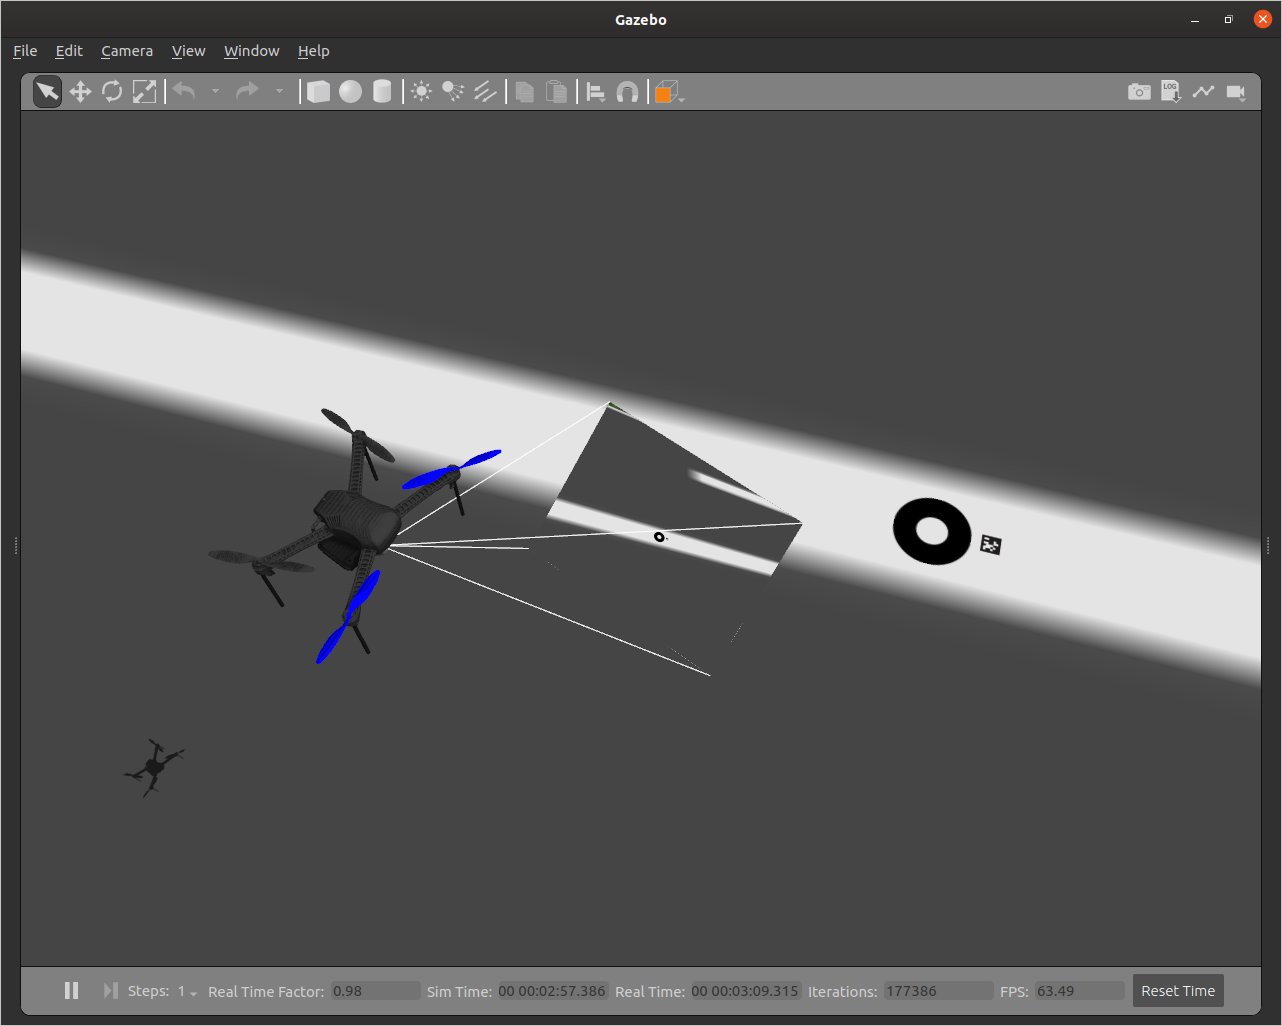
\includegraphics[width=0.8\textwidth]{images/gimbal_controller.png}
    \caption{Illustration of the drone after detecting the landing pad.}
    \label{fig:camera_offset}
\end{figure}

The role of the transforms in this scenario is to take into account the rotational displacement of the camera with respect to the drone's intrinsic, local axes, so that the pose of the landing pad can be calculated in terms of the drone itself. As a simple example to illustrate this point: if the camera is rotated to $\theta_{yaw}=-\frac{pi}{2}$ and $\theta_{pitch}=\frac{pi}{4}$, and a marker is detected 10 meters forward (in the camera's coordinate system), the gimbal controller generates a transform that will place the marker 10 meters to the left of the drone. Since the gimbal has only 2 degrees of freedom, the gimbal controller can generate the relevant transform using only the supplied pitch and roll topics from the gimbal controller plugin. This structure corresponds to a real world scenario wherein the gimbal has a mounted \gls{IMU} from which the corresponding values can be extracted.

Although the yaw position of the camera is a truly necessary component of determining the relative pose with a rotating gimbal, the pitch is not. A second method of pose estimation in this scenario is therefore to ``straighten'' the detected pose, so that the orientation is in the reference frame of the fiducial marker's normal vector. The result is that the marker's rotation is no longer needed in subsequent calculations, and the translational elements of the pose correspond to the distances in the 3 dimensions of a coordinate system centered on the marker. This can be accomplished by simply creating a transform whose translational element $t = <0, 0, 0>$ (no translation), and whose rotational element is the inverse of the marker's rotation in the original pose frame. After this transform is generated, a second transform corrects for the yaw displacement of the camera. In the case of a WhyCon marker which has no intrinsic origin in terms of yaw, a second transform corrects for the yaw displacement of the camera by adding a rotation equal to the inverse of the camera's yaw. In the case of a WhyCode or April Tag marker which do intrinsically have unambiguous yaw orientations in their pose, the yaw used to correct the pose is equal to the difference between the gimbal's yaw displacement and the marker's yaw displacement. The inverse of this value is the rotational component of the second transform. If $\theta_1$ represents the yaw of the camera, $\theta_2$ represents the yaw of the marker, and $\theta_c$ represents the yaw used to correct the pose, then $\theta_c$ can be simply calculated as follows in equation \ref{equation:yaw_correction}. In the case of a WhyCon marker, $\theta_2$ is just 0.

\begin{figure}[ht]
    \centering
    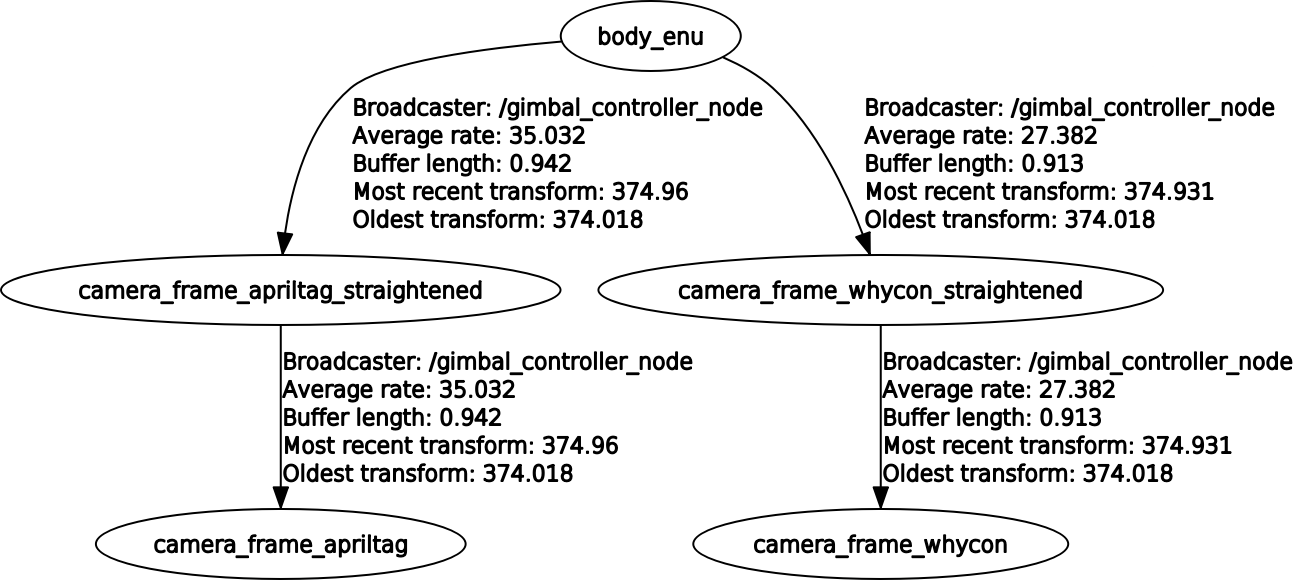
\includegraphics[width=0.7\textwidth]{images/transform_tree.png}
    \caption{Transforms used for calculating the drone's pose relative to the landing pad.}
    \label{fig:transform_tree}
\end{figure}

Figure \ref{fig:transform_tree} shows the transforms involved in calculating the drone's position relative to the April Tag or WhyCon markers. Each node contains the name of the transform frame. The function of each frame is as follows:

\begin{enumerate}
    \item \texttt{camera\_frame\_apriltag}: the transform representing the pose of the April Tag marker within the camera's field of view. This is taken from the April Tag ROS module which is analyzing the camera's published image.
    \item \texttt{camera\_frame\_apriltag\_straightened}: the transform representing the April Tag's pose when transformed to have a rotation quaternion of $\left( x, y, z, w \right) = \left( 0, 0, 0, 1 \right)$. This essentially gives the pose of the camera with respect to the marker. If the rotation of the April Tag marker in the camera's field of view is $r_a$, then this transformation composes a rotation of $r_a^{-1}$. In this case, since the April Tag's pose has unambiguous yaw, the yaw is included in this calculation.
    \item \texttt{camera\_frame\_whycon}: the transform representing the pose of the WhyCon marker within the camera's field of view. Since the WhyCon marker does not have an unambiguous yaw position, this aspect of the pose is ignored. This is taken from the WhyCon ROS module which is analyzing the camera's published image.
    \item \texttt{camera\_frame\_whycon\_straightened}: the transform representing the pose of the camera with respect to the WhyCon marker. This is calculated similarly to the straightened April Tag transform, but without considering the yaw of the marker. 
    \item \texttt{body\_enu}: the pose of the drone itself with respect to either the WhyCon or April Tag marker. This is calculated by composing the yaw component of the gimbal's rotation onto the previously straightened transforms. The relative displacement from the marker to the drone can be used in further calculations after it is transformed in this way. It is put in the \gls{ENU} coordinate frame in order to conform to the MAVROS standard.
\end{enumerate}

The transform library TF2 (used here) is the standard ROS transform library and provides an efficient means of keeping track of all published transforms 

\begin{equation}
    \theta_c = -\left( \theta_1 - \theta_2 \right)
    \label{equation:yaw_correction}
\end{equation}

When the drone is far from the landing pad and only the WhyCon marker can be identified, the gimbal controller cannot determine any information about the yaw orientation of the landing platform. This is because the WhyCon marker has rotational symmetry. Initially, the landing platform was made up of a WhyCode marker which can allow for determination of the marker's yaw orientation. However, this led to complications and was eventually abandoned for this project, as will be explained in Section \ref{subsection:whycode_trials}. The current landing platform design, using a WhyCon marker for recognition of the landing pad from a far distance, and an April Tag marker for close-range descent and accurate pose estimation, is sufficient for this project.

\section{Landing Controller}
\label{subsection:landing_controller}

\subsection{Overview}
The landing controller is a \gls{ROS} module which controls the drone's approach and descent towards the landing platform. It subscribes to data topics published by the gimbal controller, such as the relative displacement of the landing pad with respect to the drone. Then the landing controller determines the commands to send to ArduPilot in order to direct the drone towards the landing pad. It communicates with ArduPilot via a separate \gls{ROS} module called \texttt{MAVROS}, the sole purpose of which is to act as a connector between \gls{ROS} modules and any vehicle using the MAVlink communication protocol. The \texttt{MAVROS} module opens the relevant \gls{UDP} or \gls{TCP} connections with instances of MAVlink-enabled software and enables transmission of data to and from these connections via \gls{ROS} topics. These connections allow the landing controller to send control commands to the drone in the language of the flight controller, without changing the software on the flight controller.

\subsection{Data Flow}

\begin{figure}[ht]
    \centering
    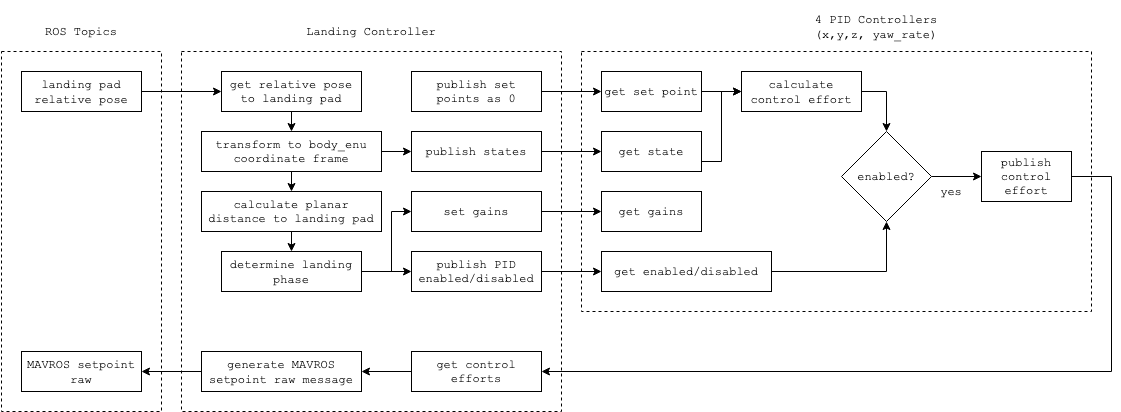
\includegraphics[width=\textwidth]{images/landing_controller.png}
    \caption{Data flow for the landing controller.}
    \label{fig:landing_controller_data_flow}
\end{figure}

The data flow for the landing controller is shown in Figure \ref{fig:landing_controller_data_flow}. The landing controller subscribes to a ROS topic containing the relative pose from the drone to the landing pad. It then transforms this pose from the camera's coordinate frame to the drone's local coordinate frame, using transforms that are also published by the gimbal controller. The landing controller publishes the states for each linear component of the displacement to each of the PID controllers. It also continually publishes the set points for the PID controllers - each with a value of 0. The planar distance to the landing pad is calculated from the relative pose, and this subsequently determines the landing phase and therefore the gains of the PID controllers and whether the PID controllers should be enabled or disabled. The PID controllers subscribe to this data, calculate the corresponding control efforts and publish the control efforts if they are enabled. Finally, the landing controller subscribes to the control effort topics, generates a message to be consumed by MAVROS, and publishes that message.

\subsection{Velocity PID Controllers}

\gls{PID} controller instances control the velocity of the drone in 4 axes that are local to the drone: east, north, up, and yaw (positive yaw is clockwise). The state values for these controllers are the component of the drone's displacement from the landing pad in the relevant axis. Since the goal of the landing controller is to direct the drone towards the landing pad - in other words, to decrease the magnitude of the displacement - the landing controller continually publishes 0 as the set point to each of these controllers when they are active. A control policy both enables/disables these controllers and changes the gains of these controllers based on the phase of the landing process. The \gls{PID} controllers publish their ``control effort'' topics after receiving data on their state and set point topics. These control effort topics are of course determined according to their gains. The landing controller subscribes to the control effort topics and translates these into a control message which is passed to ArduPilot via MAVROS.

\subsection{MAVROS Interface}

MAVROS handles communication between ROS and ArduPilot by translating ROS topics into MAVLink messages. For controlling position, velocity, and acceleration set points, the topic of interest is \texttt{/mavros/setpoint\_raw/local}. This topic allows ROS to forward the target velocities that are calculated by the PID controllers to the drone itself. This does mean that there are two sets of PID controllers - one set which calculates the target velocities, and one set that realizes these target velocities by setting the lower-level \gls{PWM} throttle signals on the drone itself, while interfacing with the \gls{IMU} to control otherwise unspecified targets such as attitude, acceleration, etc. This abstraction from the low-level commands is what allows the landing controller to be portable to different drone models and frames. The drone's intrinsic PID controllers which maintain the stable, controllable flight of the drone are tuned for their specific tasks, and the higher level PID systems are tuned for the specific task of realizing an efficient and safe trajectory towards the landing platform.

Listing \ref{lst:set_velocity_target_neu} shows the method for sending the control message to the drone. The target velocity and yaw rate represent the control effort variables calculated by the PID controllers. The \texttt{/mavros/setpoint\_raw/local} topic receives a message of type \texttt{PositionTarget}, for which a buffer has been declared. The message is stamped with the current time and tagged with the frame identifier of ``world.'' Multiple coordinate frames are available for the interpretation of the set points, but the only relevant one for this project is the coordinate frame that is local to the drone: \texttt{FRAME\_BODY\_NED} with code 8. A type mask tells the drone which parts of the message are relevant - in this case, only the linear velocities $x,y,z$ and yaw rate are published, so a value of 1991 is used. The message is then published to the topic.
\begin{lstlisting}[style=C++,caption={The simple function that allows the landing controller to control the drone's target velocities.},captionpos=b,label={lst:set_velocity_target_neu}]
void set_velocity_target_enu( geometry_msgs::Vector3 _target_velocity,
                              double _target_yaw_rate )
{
	mavros_msgs::PositionTarget buffer;

	buffer.header.stamp = ros::Time::now();
	buffer.header.frame_id = "world";
	buffer.coordinate_frame = 8; // FRAME_BODY_NED
	buffer.type_mask = 1991; // only use velocity x, y, z, yaw_rate

	buffer.velocity.x = _target_velocity.x;
	buffer.velocity.y = _target_velocity.y;
	buffer.velocity.z = _target_velocity.z;

	buffer.yaw_rate = _target_yaw_rate;

	setpoint_raw_local_publisher.publish(buffer);
}
\end{lstlisting}

There is some tedium in this setup which must be considered. First, the standard coordinate system within Gazebo is \gls{NWU}, while the standard coordinate system within MAVlink is \gls{NED}. While these are both right-handed coordinate systems and therefore a ``typical'' and simple transformation (a rotation by $\pi$ radians about the N axis) can be used, it is easier to manually change the signs of the corresponding components of the target velocity vector. Further, although MAVLink typically uses the \gls{NWU} coordinate system, MAVROS itself takes the target velocity vector in the \gls{ENU} coordinate system, which is not necessarily obvious from the documentation. However, when these aspects are accounted for, the software works as intended.

% \subsection{\color{red}Sensor Fusion and Filtering}

% {\color{red}Here I will discuss the method for sensor fusion likely using the \texttt{robot\_localization} or \texttt{robot\_pose\_ekf} ROS packages. I have attempted to use these packages already but failed to get decent results. After some time the ``filtered'' pose estimates start having a lot of spikes and become incredibly inaccurate. The goal is to be able to fuse the WhyCon, April Tag, and IMU sensor readings into a single landing pad estimate.}

\subsection{Control Policy}
\label{subsection:control_policy}

The landing controller enables/disables the PID controllers and changes their gains depending on conditions during the landing process. Initially the drone's velocity controllers have high P-gains and low D-gains. This allows the drone to approach the landing pad quickly from far distances. As the drone gets closer to the landing pad, the I and D gains become more important and are set to experimentally-determined values (presented in Section \ref{subsection:pid_tuning}) to avoid the quintessential PID overshoot and instead conserve battery and time. The standard ROS PID module has been slightly modified to allow the gains to be reconfigured quickly using a single topic, rather than the existing method of using \texttt{rqt\_reconfigure} which requires a separate module and which seems to react slowly to the reconfiguration.\footnote{The original PID module code can be found at \url{https://bitbucket.org/AndyZe/pid/src/master/} and the slightly edited version can be found at \url{https://github.com/uzgit/pid}.}

Although a drone can move in any direction, it is necessary to control the yaw of the drone during descent, as the legs of the drone can obstruct the tracked fiducial marker. Although WhyCon markers tend to be robust to minor obstructions, the more intricate April Tag markers are not. The Iris, for example, has a black airframe which can merge with the black boundary and tiles of April Tag markers in the field of view of the camera, forming a contiguous black region which does not conform to the required structure of April Tag markers and prevents April Tag identification. Figure \ref{fig:obstruction} illustrates this point. In Figure \ref{subfig:apriltag_not_obtructed}, the April Tag marker is clearly identified (hence the ID is printed on the screen) even at a somewhat high angle of deflection, but in Figure \ref{subfig:apriltag_obtructed}, the slight intersection of the drone's leg with the April Tag marker prevents identification. In this case, yaw correction  ensures that the drone is aligned to the landing platform in such a way that the April Tag marker is unobstructed by the drone itself throughout the descent. However, yaw correction is only allowed once the April Tag marker has been identified, since the April Tag marker is the only marker on the landing pad which provides a yaw orientation. In contrast to April Tag's obvious sensitivity, Figure \ref{fig:whycon_robust} shows the robustness of WhyCon identification. The shadow of the drone forms a contiguous black region extending the WhyCon marker's black region. (White and black are inverted in the picture in order to make the detection more clear.) However, the WhyCon system still correctly identifies the marker and places its center in the correct location, as shown by the very faint green and red dots.

\begin{figure}[ht]
    \centering
    \begin{subfigure}[b]{0.49\textwidth}
        \centering
        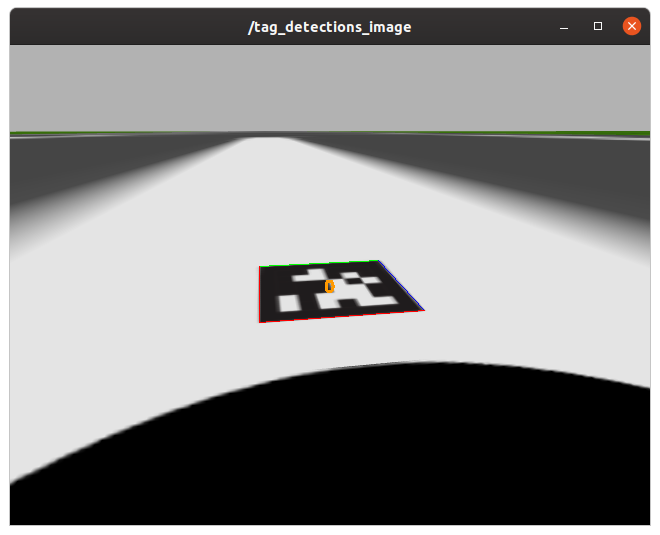
\includegraphics[width=\textwidth]{images/apriltag_not_obstructed.png}
        \caption{April Tag not obstructed, and therefore successfully identified.}
        \label{subfig:apriltag_not_obtructed}
    \end{subfigure}
    \begin{subfigure}[b]{0.49\textwidth}
        \centering
        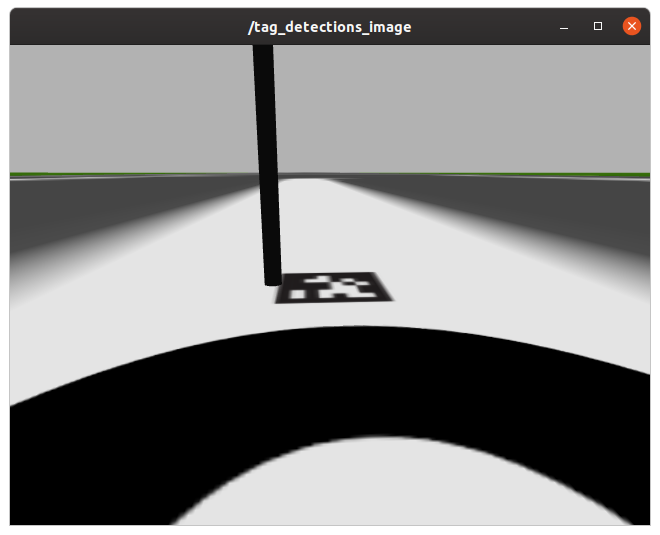
\includegraphics[width=\textwidth]{images/apriltag_obstructed.png}
        \caption{April Tag slightly obstructed, and therefore not identified at all.}
        \label{subfig:apriltag_obtructed}
    \end{subfigure}
    \caption{Even slight obstructions can prevent identification of April Tag markers.}
    \label{fig:obstruction}
\end{figure}

\begin{figure}[ht]
    \centering
    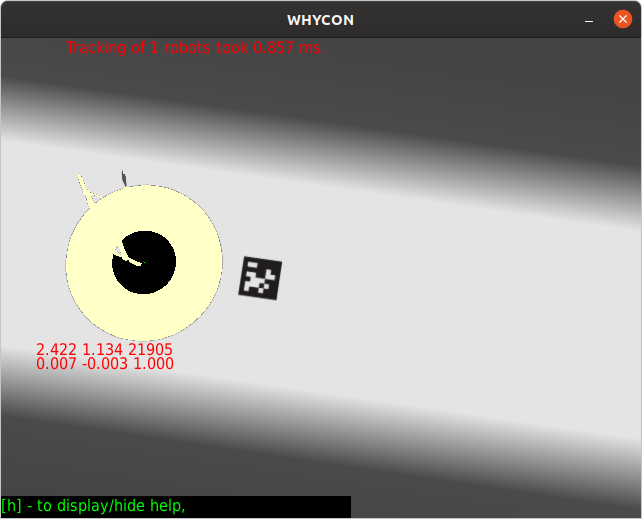
\includegraphics[width=0.5\textwidth]{images/whycon_robust.png}
    \caption{WhyCon identification is robust even to significant obstructions.}
    \label{fig:whycon_robust}
\end{figure}

Finally, descent is allowed or disallowed based on a dynamic threshold $\delta$ on the planar distance $d_p$ to the landing pad. This threshold follows an exponential function as outlined in Equation \ref{equation:plane_distance_threshold}:

\begin{equation}
    \delta = k_1e^{k_2 z}
    \label{equation:plane_distance_threshold}
\end{equation}
where
\begin{itemize}
    \item $\delta$ is the planar distance threshold, below which the drone is allowed to descend,
    \item $k_1$ and $k_2$ are constants determined through exponential fitting of a curve to experimentally-determined constraints, and
    \item $z$ is the vertical distance from the drone to the landing pad, or equivalently the altitude of the drone above the landing pad.
\end{itemize}

The drone is allowed to descend if $d_p = \sqrt{x^2 + y^2} < \delta$, where $x$ and $y$ are the distances from the drone to the landing pad in the drone's East and North axes respectively. This means that, the higher the drone is above the landing pad, the farther away it is allowed to descend. Conversely, the lower the altitude of the drone, the closer the drone must be to landing pad in order to descend - ensuring that the drone does not descend to the ground in any place except for the landing pad. This is visualized in Figure \ref{fig:descent_region}, where the descent region is the interior of the plotted surface. The motivation for this is that, with the movements and vibrations of the drone - and the inherent inaccuracies in monocular pose estimation - the drone is able to better estimate its pose when it is closer to the landing pad (e.g. after it has partially descended). The specific landing phases are outlined in Table \ref{tab:landing_phases}.

\begin{figure}[h]
    \centering
    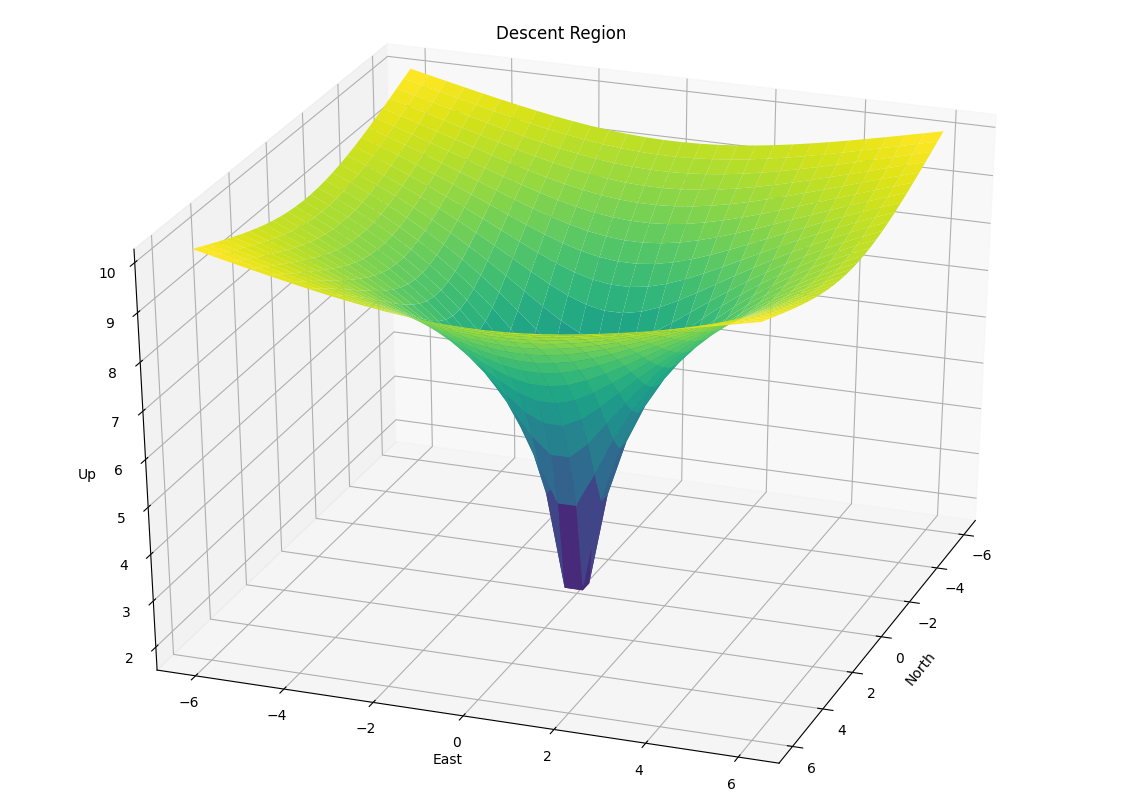
\includegraphics[width=0.75\textwidth]{images/descent_region.png}
    \caption[Example descent region.]{An example descent region for a $k_1=0.15, k_2=0.4$, with the landing platform positioned at $(x,y,z)=(0, 0, 0)$. The drone is allowed to descend in the interior of the plotted surface.}
    \label{fig:descent_region}
\end{figure}

% \begin{etaremune}
%   \item \texttt{NOT\_LANDING}: This is the mode set when the landing controller has been disabled or the landing pad is not yet recognized. Setting this mode triggers a target velocity of 0 in all dimensions, effectively aborting an ongoing landing. This can happen if the user disables the landing or if the landing pad leaves the field of view of the camera for a specified abort time.
%   \item \texttt{APPROACH}: This mode is the first mode set when the landing controller is enabled and the landing pad is located. This mode uses high P-gain, and low D-gain for a quick initial approach, and a 0 I-gain in order not to bias the drone's final velocity.
%   \item \texttt{CLOSE\_APPROACH}: This mode is set once the drone's planar distance to the landing pad is less than some experimentally-determined multiple of the descent distance. The P-gain is lowered and the D-gain is raised in order to gradually slow the drone's approach. The I-gain is still set to 0 at this point. The motivation for this landing phase is to avoid the drone overshooting the landing pad after a quick initial approach.
%   \item \texttt{YAW\_CORRECTION}: During this mode, the drone's yaw PID controller is enabled, which allows the drone to align itself with the landing pad so that the drone's body does not obscure the April Tag marker during final descent. The P-gain of the east and north PID controllers is reduced yet again, and the D-gain increased, in order to avoid overshoot. Descent to some minimum altitude is allowed during this phase, however full descent is not allowed until the drone is aligned within 5 degrees of the landing pad's orientation.
%   \item \texttt{DESCENT}: During this mode, the yaw PID controller is disabled and the heading of the drone is locked by setting its target yaw velocity to 0. Descent below the previously mentioned minimum altitude is allowed. The PID controllers in the north, east, and up directions are still enabled for final velocity correction.
%   \item \texttt{LANDED}: All PID controllers are disabled, east and north target velocities are preserved and continually sent as velocity targets to the drone. The target velocity in the up direction is set to some constant negative value and also sent to the flight controller.
% \end{etaremune}

\begin{table}[h!]
    \centering
    \begin{tabular}{|l|p{12cm}|}
    \hline
        \texttt{NOT\_LANDING} & This is the mode set when the landing controller has been disabled or the landing pad is not yet recognized. Setting this mode triggers a target velocity of 0 in all dimensions, effectively aborting an ongoing landing. This can happen if the user disables the landing or if the landing pad leaves the field of view of the camera for a specified abort time. \\\hline
        \texttt{APPROACH} & This mode is the first mode set when the landing controller is enabled and the landing pad is located. This mode uses high P-gain, and low D-gain for a quick initial approach, and a 0 I-gain in order not to bias the drone's final velocity. \\\hline
        \texttt{CLOSE\_APPROACH} & This mode is set once the drone's planar distance to the landing pad is less than some experimentally-determined multiple of the descent distance. The P-gain is lowered and the D-gain is raised in order to gradually slow the drone's approach. The I-gain is still set to 0 at this point. The motivation for this landing phase is to avoid the drone overshooting the landing pad after a quick initial approach. \\\hline
        \texttt{YAW\_CORRECTION} & During this mode, the drone's yaw PID controller is enabled, which allows the drone to align itself with the landing pad so that the drone's body does not obscure the April Tag marker during final descent. The P-gain of the east and north PID controllers is reduced yet again, and the D-gain increased, in order to avoid overshoot. Descent to some minimum altitude is allowed during this phase, however full descent is not allowed until the drone is aligned within 5 degrees of the landing pad's orientation. \\\hline
        \texttt{DESCENT} & During this mode, the yaw PID controller is disabled and the heading of the drone is locked by setting its target yaw velocity to 0. Descent below the previously mentioned minimum altitude is allowed. The PID controllers in the north, east, and up directions are still enabled for final velocity correction. \\\hline
        \texttt{LANDED} & All PID controllers are disabled, east and north target velocities are preserved and continually sent as velocity targets to the drone. The target velocity in the up direction is set to some constant negative value and also sent to the flight controller. \\\hline
    \end{tabular}
    \caption{Landing Phases}
    \label{tab:landing_phases}
\end{table}

Each of the landing phases is used only to enable and disable PID controllers and change their gains. However there are two other, redundant checks performed at every iteration of the landing controller's loop. First, the yaw of the drone is locked if the drone's yaw is aligned within 5 degrees of the landing pad's yaw orientation. This is done simply by disabling the yaw PID controller and setting a target yaw velocity of 0. Second, if the drone is not in the \texttt{LANDED} phase, a separate check disables descent if the drone is outside of the descent region, and enables it otherwise. This is done by disabling the PID controller for the up direction and setting a target up velocity of 0, and re-enabling the PID controller respectively.

The landing controller is enabled or disabled based on the PWM signal given on a user-defined channel. In this case, channel 11 is used, and a PWM signal on this channel with a duty cycle of more than 50\% enables the landing controller. It is disabled otherwise. This allows manual landing abort and also integration of an autonomous landing into semi-autonomous flights.

At the time of this writing, ArduPilot does not appear to have a feature which allows the sudden disarming of a drone's motors, which would be quite useful after the drone has landed. However, ArduPilot does automatically disarm the motors after it detects that the drone has landed, even when the final velocity is non-zero, and even when non-zero target velocities are set. In order to use ArduPilot without editing it, this fact is leveraged, and the motors are allowed to automatically disarm. It is important that the landing pad maintain a constant velocity until the drone disarms.



% , as shown in Figure \ref{fig:landing_system_architecture}. The first is the \texttt{roscore} module which is necessary within the \gls{ROS} framework and which functions as a base server to facilitate communication among the other \gls{ROS} modules. The data flow is as follows:

% \begin{enumerate}
%     \item The drone-mounted camera provides a raw image of the landing pad's fiducial marker.
%     \item The \texttt{usb\_cam} module provides the raw image from the camera to the rest of the \gls{ROS} modules as a topic.
%     \item The \texttt{whycon\_ros} module analyzes the camera frames and attempts to detect and identify WhyCon markers within the image. If it detects a WhyCon marker, it provides the location and rotation of the marker relative to the camera.
%     \item The \texttt{landing\_controller} module monitors the position of the fiducial marker over time, simultaneously determining the relative velocity. It generates an approach trajectory and communicates this in the MAVlink protocol to the ArduPilot software via the \texttt{mavros} module.
%     \item The \texttt{abort\_controller} module continuously monitors the \gls{IMU} conditions of the drone and the visibility of the fiducial marker in order to determine whether an in-progress landing should be aborted.
%     \item The \texttt{mavros} module provides an interface to allow the \gls{ROS} modules to communicate to the ArduPilot software using the MAVlink communication protocol.
% \end{enumerate}

% \begin{figure}[H]
%     \centering
%     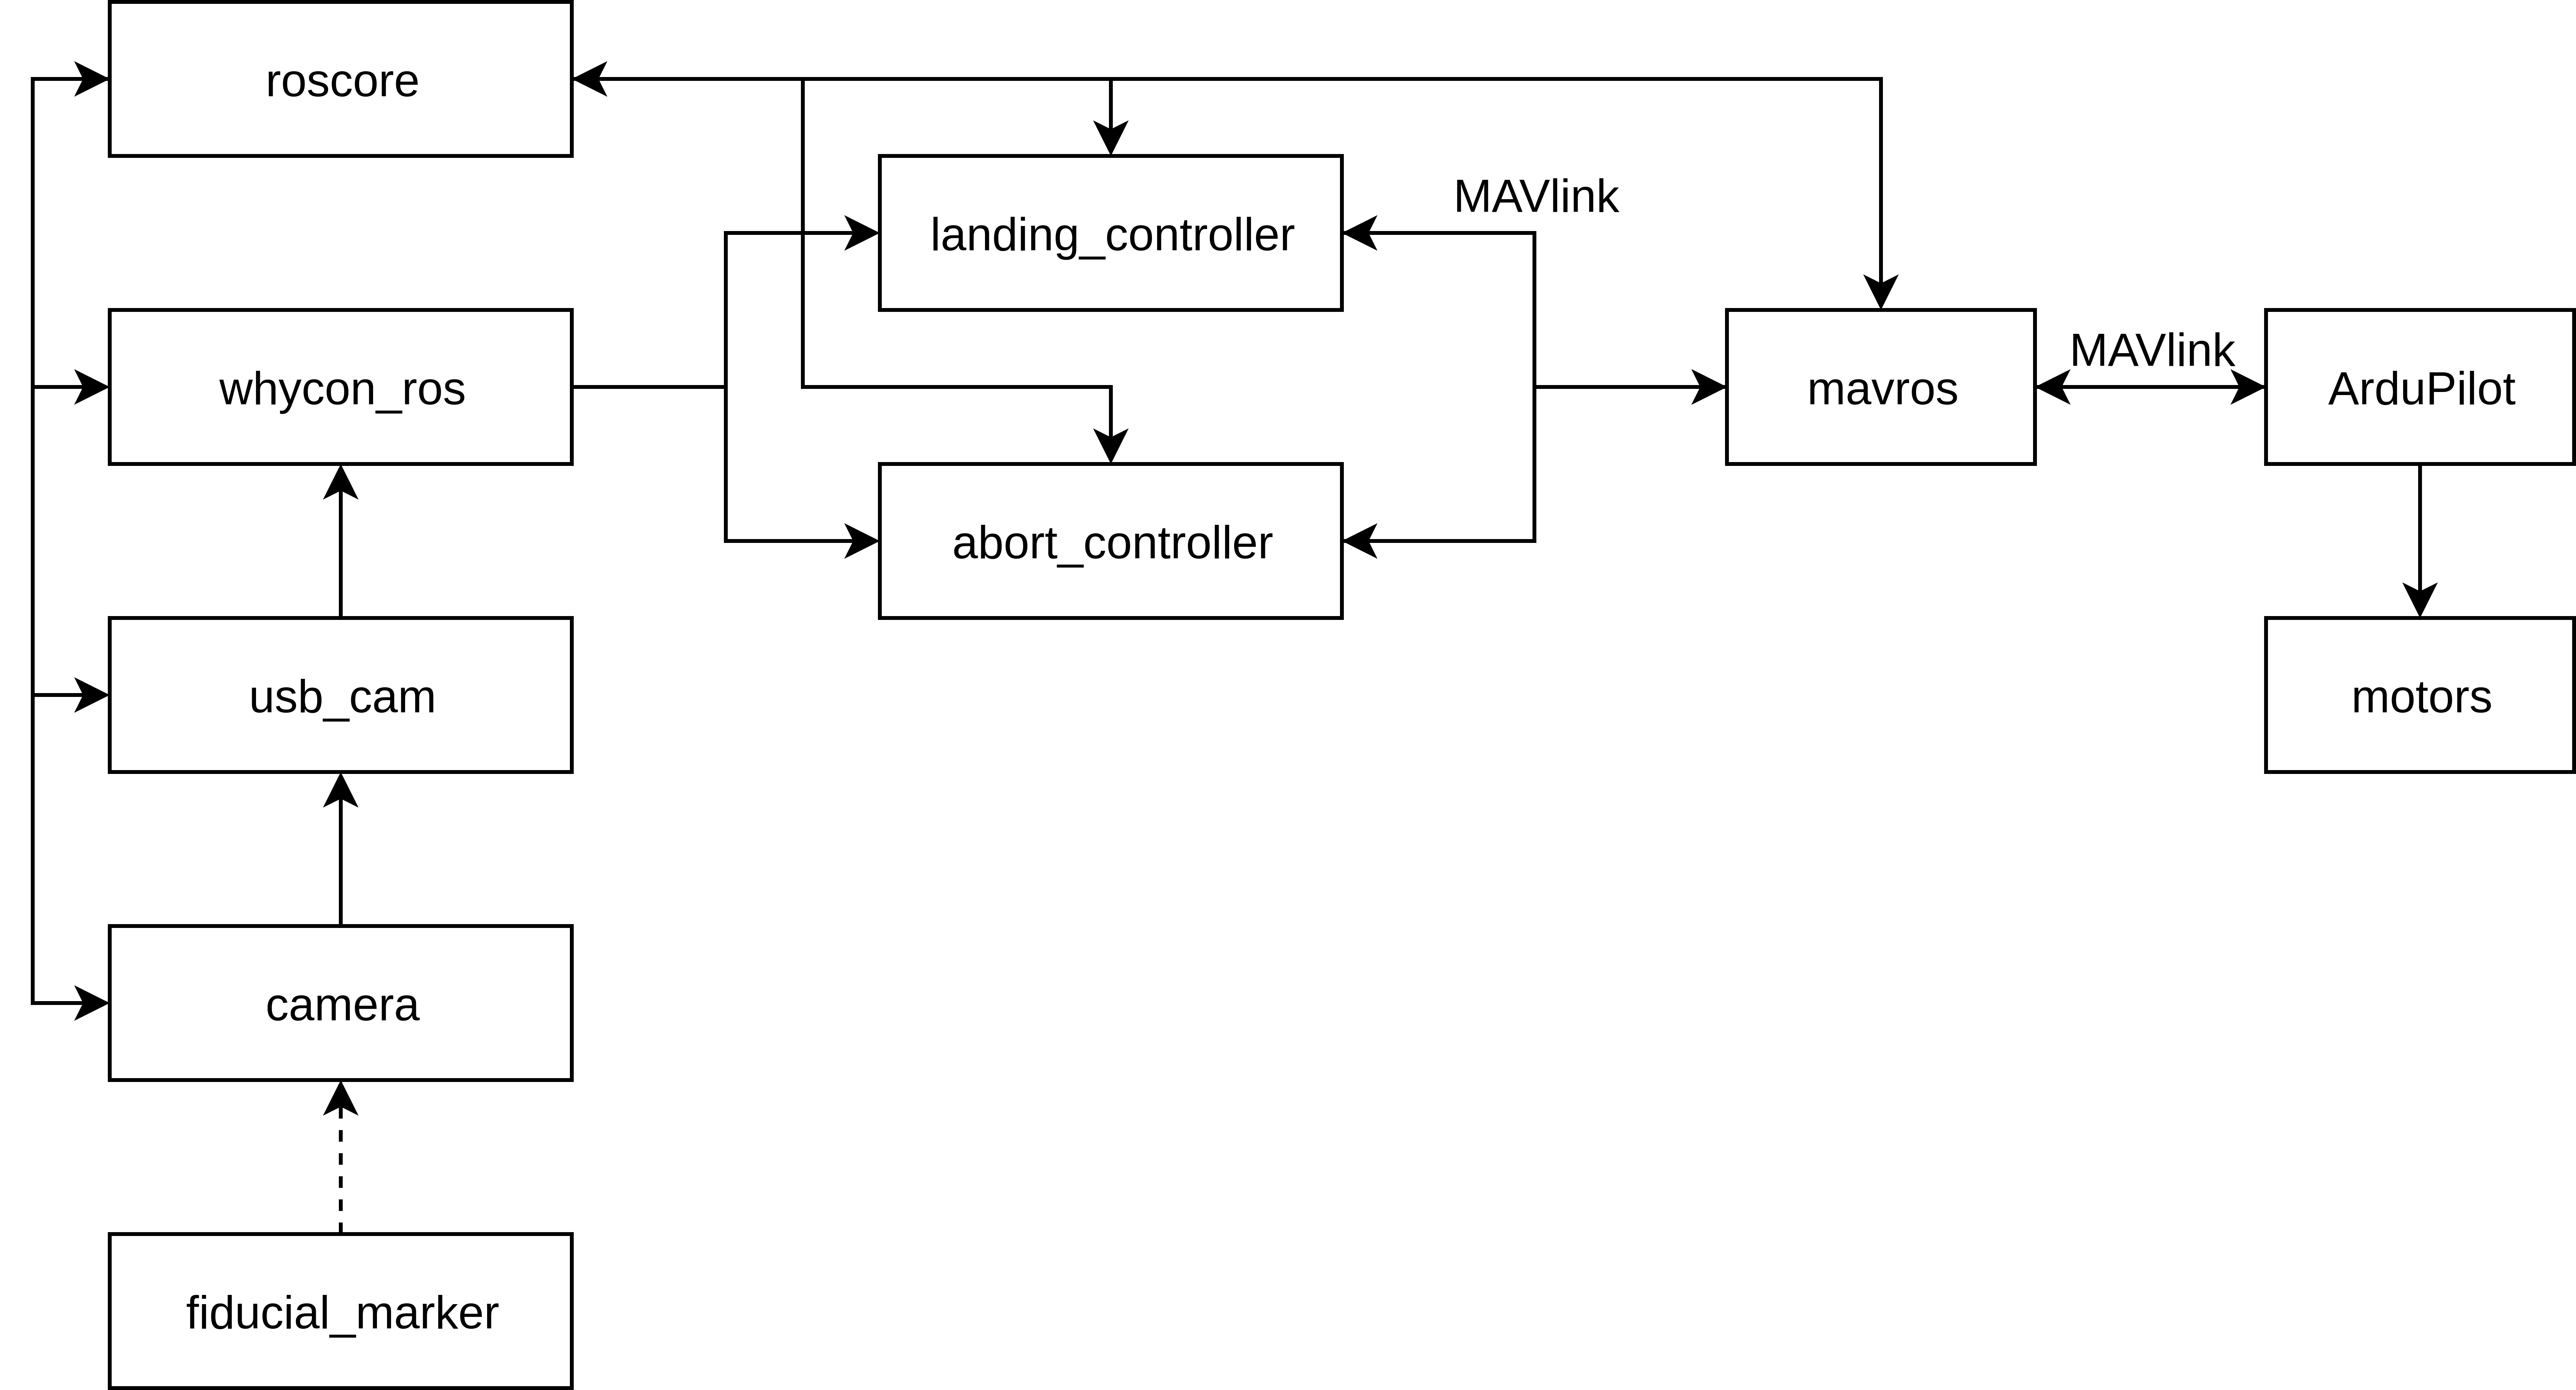
\includegraphics[width=\textwidth]{images/system_architecture.png}
%     \caption{High level landing system architecture.}
%     \label{fig:landing_system_architecture}
% \end{figure}

\chapter{Simulation Results}
\label{chapter:simulation_results}
\section{Simulated Camera Calibration}
\label{section:camera_calibration}

As described in Section \ref{subsection:setup_and_tools}, a standard Gazebo ROS camera sensor is ``mounted'' to the Iris' gimbal and provides a simulated camera image as a ROS topic. The important aspects of this code are the specifications for the camera's distortion coefficients, which are all set to 0.0. Any library using a camera for image processing will require these values. Instead of passing these values to the WhyCon and April Tag libraries directly, the \texttt{calibrate\_camera} ROS module was used to generate a \texttt{.yaml} file containing the empirically determined values. This method is a de facto standard way of calibrating a camera in ROS, and can be used during migration to a physical system.
% \begin{lstlisting}[style=XML,caption={Instantiation of a Gazebo ROS camera sensor.},captionpos=b,label={lst:camera_sensor_instantiation}]
% <plugin name="camera_controller" filename="libgazebo_ros_camera.so">
%     <alwaysOn>true</alwaysOn>
%     <updateRate>0.0</updateRate>
%     <robotNamespace>/</robotNamespace>
%     <cameraName>camera</cameraName>
%     <imageTopicName>image_raw</imageTopicName>
%     <cameraInfoTopicName>camera_info</cameraInfoTopicName>
%     <frameName>camera_link</frameName>
%     <distortionK1>0.0</distortionK1>
%     <distortionK2>0.0</distortionK2>
%     <distortionK3>0.0</distortionK3>
%     <distortionT1>0.0</distortionT1>
%     <distortionT2>0.0</distortionT2>
% </plugin>
% \end{lstlisting}
%<hackBaseline>0.07</hackBaseline>
The \texttt{calibrate\_camera} script requires a rectangular ``chessboard'' defined by $m-1$ and $n-1$ where $m$ is the amount of squares along one side, and $n$ is the amount of squares along a perpendicular side. This chessboard was inserted into \texttt{sandbox.world} as a texture, as shown in Figure \ref{fig:camera_calibration}. The sizes of the squares in the chessboard are an important factor in calibration, and they were approximately the size of a single 1-meter grid square. The drone was directed around the chessboard in order to view it from many angles and distances, after which a calibration file was generated.

\begin{figure}[ht]
    \begin{subfigure}[b]{0.48\textwidth}
        \centering
        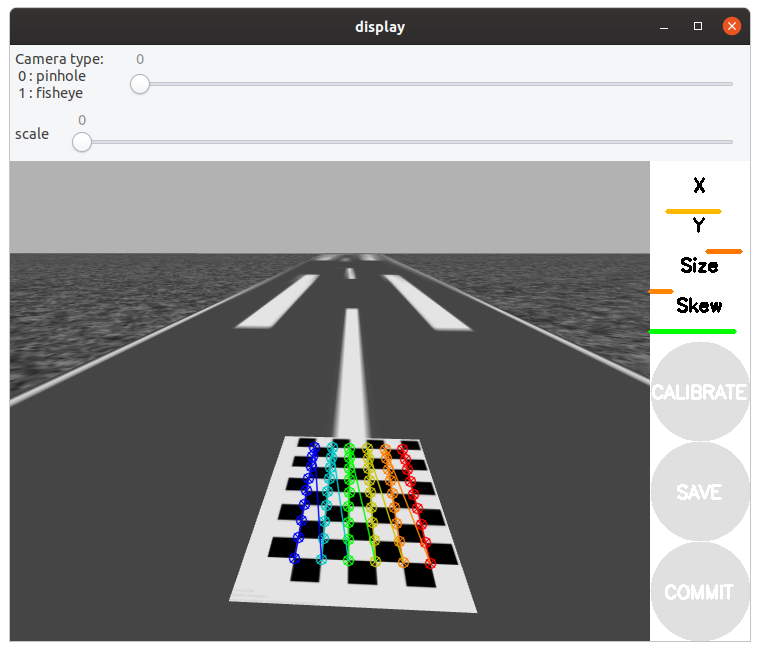
\includegraphics[height=5cm]{images/calibration_camera_view.png}
        \caption{``Chessboard'' detection.}
        \label{subfig:calibration_camera_view}
    \end{subfigure}
    \begin{subfigure}[b]{0.48\textwidth}
        \centering
        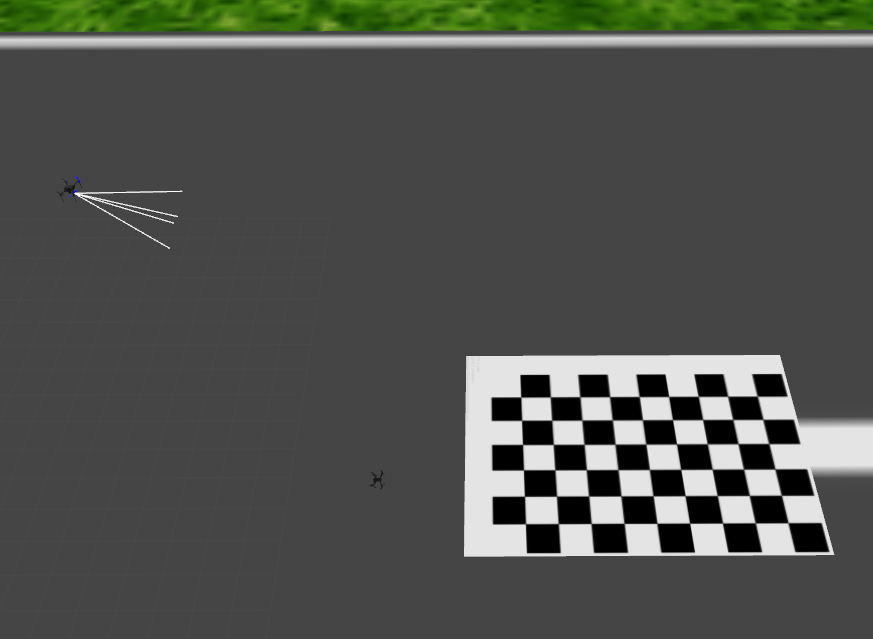
\includegraphics[height=5cm]{images/calibration_birds_eye_view.png}
        \caption{The calibration ``chessboard'' from above.}
        \label{subfig:calibration_birds_eye_view}
    \end{subfigure}
    \caption{Calibration of the simulated camera.}
    \label{fig:camera_calibration}
\end{figure}

The calibration generated the following data which has been rounded for conciseness. The camera intrinsics matrix $K$ contains $f_x, f_y$ which are the focal lengths of the camera in the $x$ and $y$ dimensions respectively, in pixel units. It also contains $c_x, c_y$ which represent the coordinates of a principal point that should be near the image center. After calibration, the simulated camera sensor is calculated to have focal lengths $f_x, f_y$ of 398.2 and 390.8 pixels respectively. With a resolution of 640x480 pixels, the calibrated values of $c_x=299.9$ and $c_y=227.5$ are only \textit{near} the image center - slightly to the upper left.

\begin{equation}
    K=
    \begin{pmatrix}
        f_x & 0 & c_x\\
        0 & f_y & c_y\\
        0 & 0 & 1
    \end{pmatrix}
    =
    \begin{pmatrix}
        398.2 & 0 & 299.9\\
        0 & 390.8 & 227.5\\
        0 & 0 & 1
    \end{pmatrix}
    \label{equation:camera_intrinsic_matrix}
\end{equation}

The distortion coefficients determined by the camera calibration, $D_T$, are roughly equivalent to those set in the camera plugin's parameters. The radial distortion coefficients $k_1, k_2, k_3$ are set to exactly zero but are calculated as only near-zero after the calibration. The tangential distortion coefficients $p_1, p_2$, corresponding to T1 and T2 in the camera plugin parameters, are also non-zero but near-zero.

\begin{equation}
    D^T=
    \begin{pmatrix}
        k_1\\k_2\\p_1\\p_2\\k_3
    \end{pmatrix}
    =
    \begin{pmatrix}
        0.0576\\-0.0321\\0.0041\\-0.0203\\0
    \end{pmatrix}
    \label{equation:distortion_coefficients}
\end{equation}

It is important to note that the process of calibrating the camera module has been developed out of necessity because typical real world cameras have non-negligible distortion coefficients. The values determined for $D^T$ are significantly lower in magnitude than those of a typical, real camera. 

% The rotation matrix $R$ determines the rotation between the first and second cameras in a stereo-vision setup. In this monocular case, the rotation is 

% \begin{equation}
%     R=
%     \begin{pmatrix}
%         1 & 0 & 0\\
%         0 & 1 & 0\\
%         0 & 0 & 1
%     \end{pmatrix}
%     \label{equation:rectification_matrix}
% \end{equation}

% \begin{equation}
%     P=
%     \begin{pmatrix}
%         406.9 & 0 & 282.8 & 0\\
%         0 & 412.1 & 229.92 & 0\\
%         0 & 0 & 1 & 0
%     \end{pmatrix}
%     \label{equation:projection_matrix}
% \end{equation}


\section{Gimbal Controller}
\label{section:gimbal_controller_results}

As stated in Section \ref{subsection:aiming_the_camera}, the main job of the gimbal controller is to aim the camera directly at the landing platform. It does this by using 2 PID controllers - one on its pitch angle and one on its yaw angle - to control its 2 degrees of freedom. Initially, PD controllers were used for this purpose, but they were inadequate as the simulated gimbal has spring forces which tend to keep the gimbal's positions at their original points. As the magnitude of the pitch or yaw angles increases, the force required to further increase the angle's magnitude increases. Over time, a small integral gain helps correct the error caused by this change in required force. Table \ref{tab:gimbal_controller_pid_gains} shows the gains for the gimbal PID controllers.

\begin{table}[ht]
    \centering
    \begin{tabular}{|c|c|c|c|}
    \hline
        Controller & $k_p$ & $k_i$ & $k_d$ \\\hline
        Pitch & 0.25 & 0.1 & 0.025 \\\hline
        Yaw & 0.25 & 0.1 & 0.025 \\\hline
    \end{tabular}
    \caption{Gimbal controller PID gains.}
    \label{tab:gimbal_controller_pid_gains}
\end{table}

The $x$ and $y$ components of the un-transformed landing platform pose comprise the input for target angle calculation, and these target angles are used as the set points for the PID controllers. The $x$ and $y$ components are scaled by a factor inversely proportional to the $z$ component in order to allow the PID controllers to function in a stable way over a variety of distances. If the $x$ and $y$ components are used without scaling, the PID controllers wildly overshoot at long distances and undershoot at short distances. Figures \ref{subfig:x_displacement} and \ref{subfig:y_displacement} show the performance of the gimbal controller during 10 landings. In both figures, each line represents a single attempt to aim camera over the course of the landing. Time $t=0$ represents that time of first recognition of the landing platform. At about 30 seconds in each landing sequences, the drone has made contact with the landing platform. The graph continues in time until the drone disarms, completing the landing. Figure \ref{subfig:x_displacement} shows that, after some oscillation, the yaw of the gimbal is adjusted so that the marker is in the center of the camera's view in the $x$ direction. Figure \ref{subfig:y_displacement} shows similar results with regards to the gimbal's pitch, but with an added, temporary bias during which time the gimbal is pointed slightly lower than the landing platform. This is because, when the drone is close to the landing pad, the April Tag marker is almost directly in front of the drone and therefore the spring resistance in the gimbal is high. The error is eventually corrected by the integral gain and the marker becomes centered in the $y$ direction of the camera frame. Centering of the landing platform in the camera's field of view is represented by the convergence of each line to 0. However, even though the ideal goal of the gimbal controller is to keep the landing platform centered in this way, it is only critical that it must keep the landing platform in the camera's field of view throughout a variety of orientations and displacements. These figures show that the gimbal controller does accomplish this goal.

\begin{figure}[ht]
    \centering
    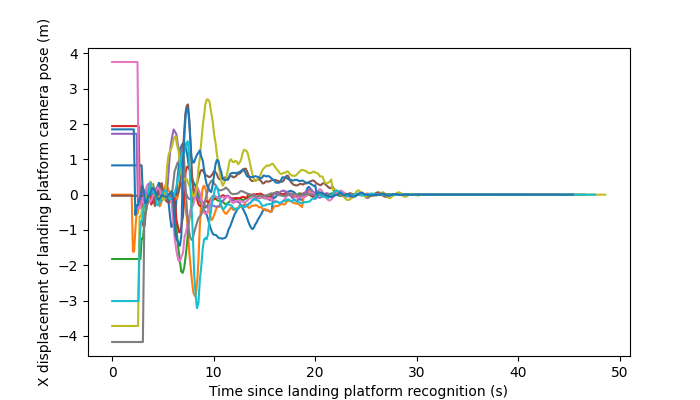
\includegraphics[width=0.7\textwidth]{images/x_displacement.png}
    \caption[Landing platform $x$ displacement in camera frame versus time.]{Landing platform $x$ displacement in camera frame versus time. Each line represents a single attempt to aim the camera during landing.}
    \label{subfig:x_displacement}
\end{figure}

\begin{figure}[ht]
    \centering
    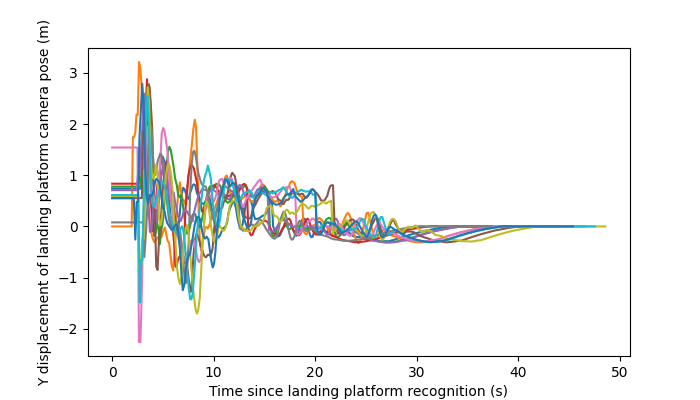
\includegraphics[width=0.7\textwidth]{images/y_displacement.png}
    \caption[Landing platform $y$ displacement in camera frame versus time.]{Landing platform $y$ displacement in camera frame versus time. Each line represents a single attempt to aim the camera during landing.}
    \label{subfig:y_displacement}
\end{figure}

% \begin{figure}[ht]
%     \centering
%     \begin{subfigure}[b]{0.47\textwidth}
%         \centering
%         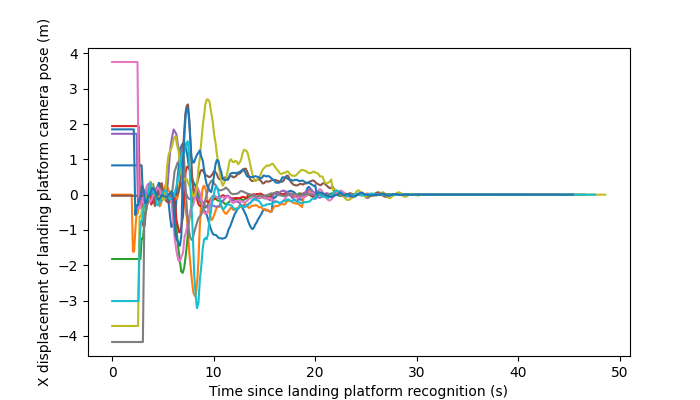
\includegraphics[width=\textwidth]{images/x_displacement.png}
%         \caption{Landing platform X displacement in camera frame.}
%         \label{subfig:x_displacement}
%     \end{subfigure}
%     \begin{subfigure}[b]{0.47\textwidth}
%         \centering
%         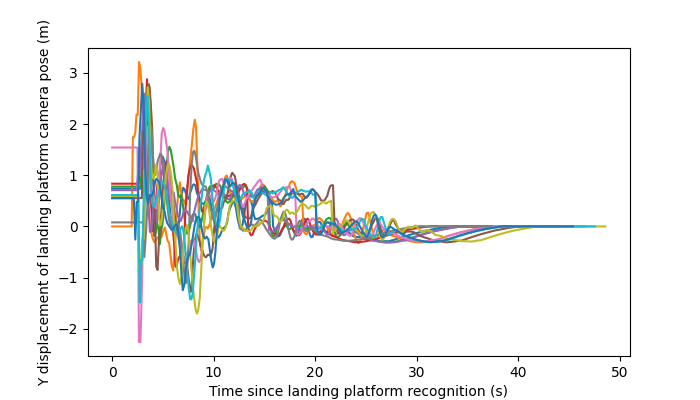
\includegraphics[width=\textwidth]{images/y_displacement.png}
%         \caption{Landing platform Y displacement in camera frame.}
%         \label{subfig:y_displacement}
%     \end{subfigure}
%     \caption{Time versus linear displacement in X and Y directions for landing platform pose in camera frame.}
%     \label{subfig:gimbal_x_y_displacement}
% \end{figure}

The pose of the landing platform in the $z$ direction behaves differently, in that it converges to some non-zero distance representing the depth of the landing platform in the camera frame. As the drone approaches the landing platform, this depth of course decreases to near-zero as the drone lands.

\begin{figure}[ht]
    \centering
    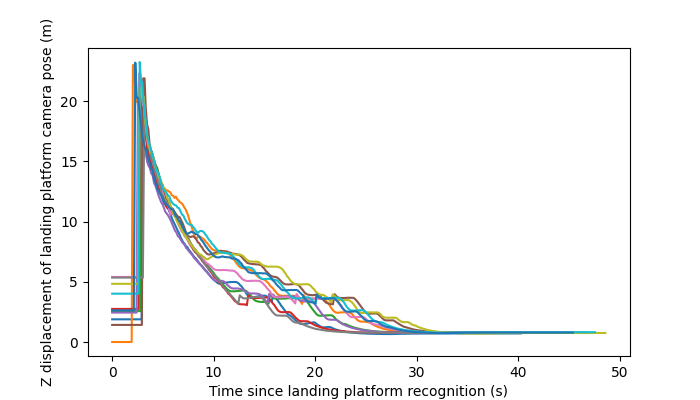
\includegraphics[width=0.7\textwidth]{images/z_displacement.png}
    \caption[Landing platform $z$ displacement in camera frame versus time.]{Landing platform $z$ displacement in camera frame versus time. Each line represents a single attempt to aim the camera during landing.}
    \label{fig:gimbal_z_displacement}
\end{figure}

\section{WhyCon Pose Estimation}

% \begin{figure}[ht]
%     \centering
%     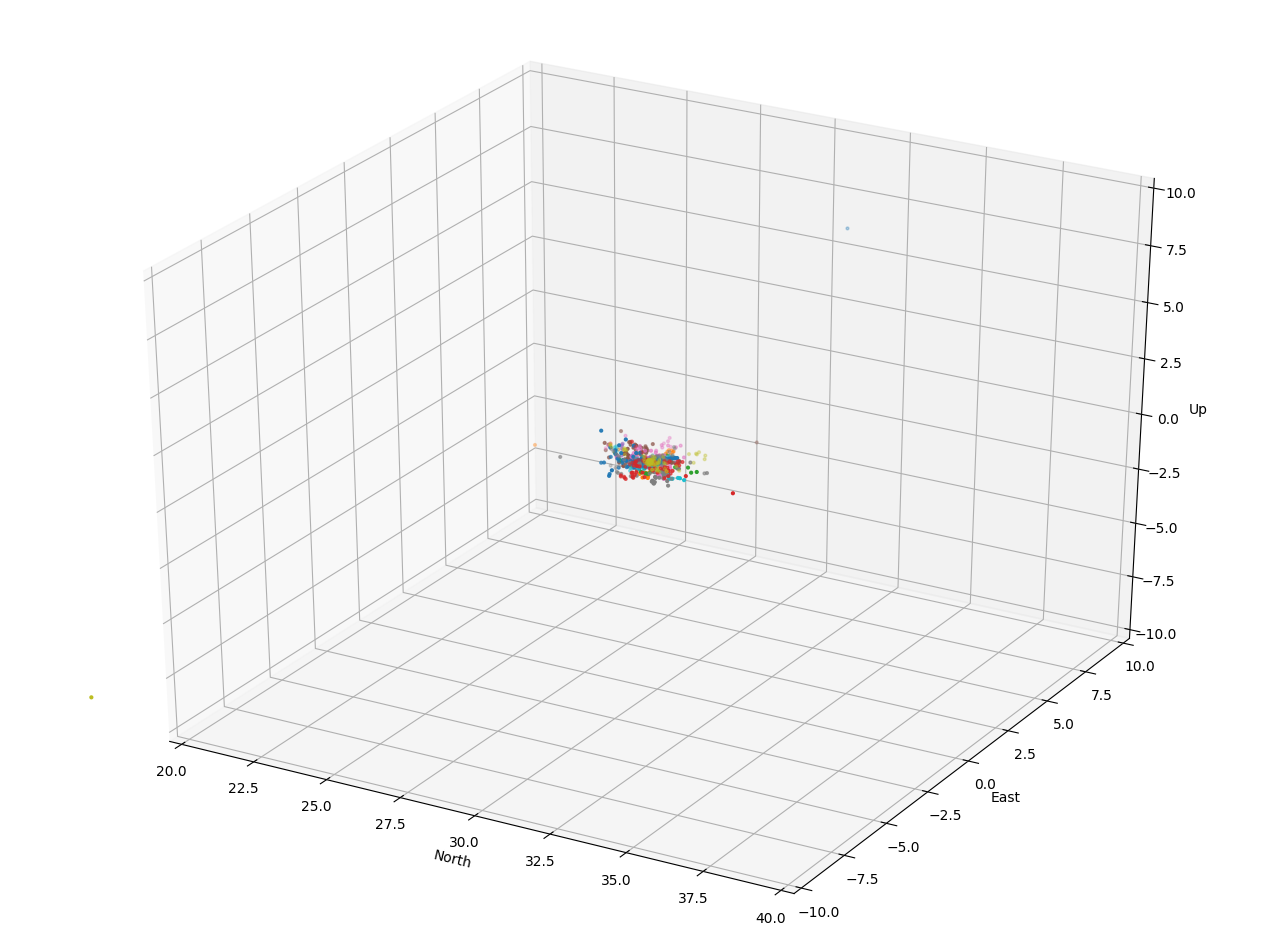
\includegraphics[width=0.9\textwidth]{images/whycon_pose_estimation.png}
%     \caption{WhyCon stationary pose estimation without outliers.}
%     \label{fig:whycon_stationary_pose_estimation}
% \end{figure}

WhyCon markers, as previously known, provide a good means of pose estimation in 3 dimensions, especially in stationary scenarios. Stationary WhyCon pose estimation was therefore the first step in testing the drone's ability to identify the landing platform's position. In configuring the WhyCon system, the outer diameter of the WhyCon marker is a required point of data. The WhyCon module makes it easy to configure this in real time using \texttt{rqt\_reconfigure}. The calibration was quite simple regardless, as the marker was intentionally sized to 1 (simulated) meter in Gazebo. The results of the system calibrated in this way are shown below.

\begin{figure}[ht]
    \centering
    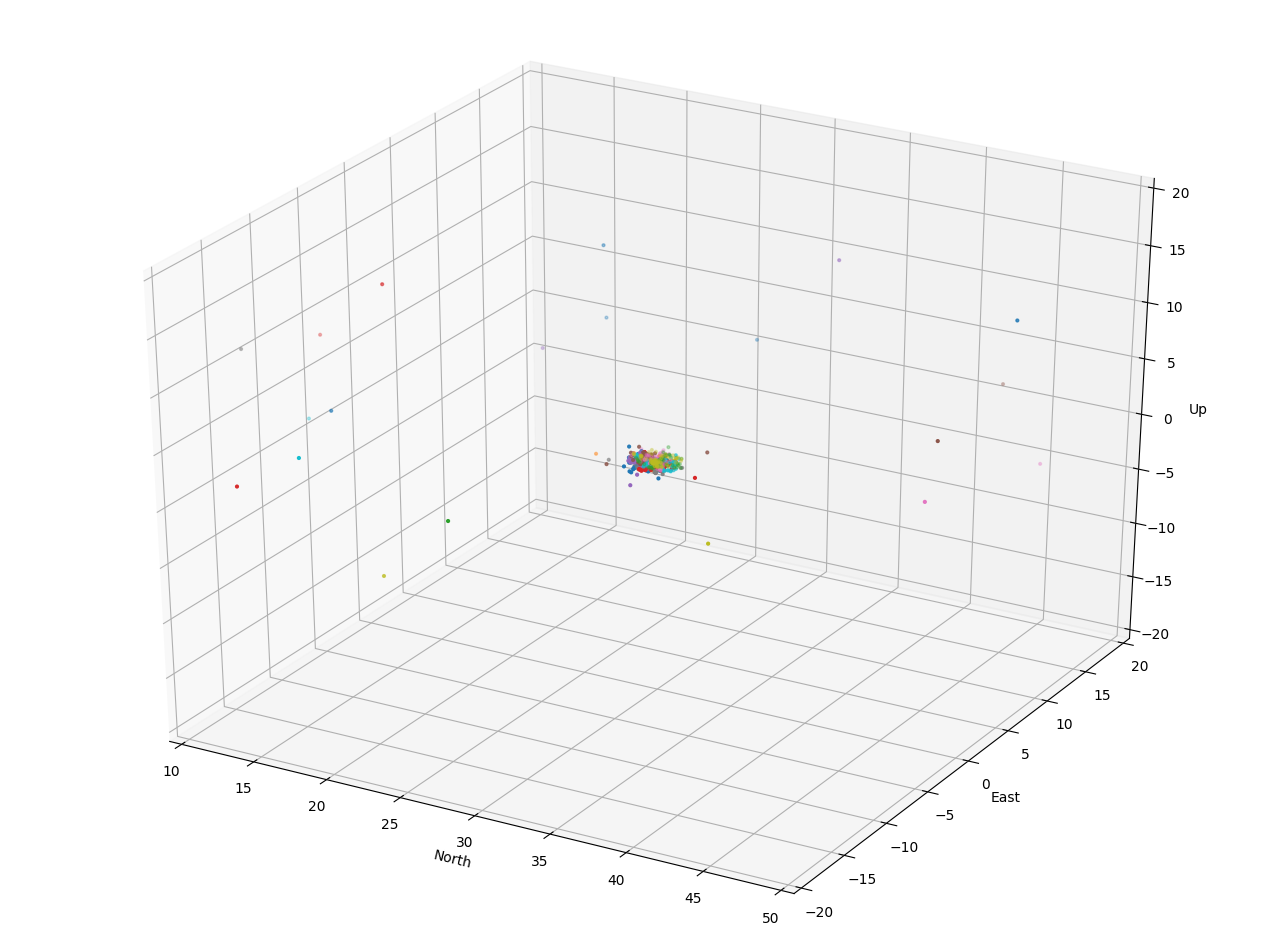
\includegraphics[width=0.85\textwidth]{images/whycon_pose_estimation_with_outliers.png}
    \caption[WhyCon stationary pose estimation with outliers included.]{WhyCon stationary pose estimation with outliers included. This shows that the majority of the poses are concentrated in a small area, and the outliers are relatively few.}
    \label{fig:whycon_stationary_pose_estimation_with_outliers}
\end{figure}

The WhyCon marker is the intended landing site of the drone. In the stationary landing scenario, it was placed at (0, 30, 0) and, as shown in Figure \ref{fig:whycon_stationary_pose_estimation_with_outliers}, the drone is able to reliably estimate the pose of the WhyCon marker. There is transient angular movement in the camera from the moment that the system recognizes the marker to the moment that the camera centers on the marker, which cannot practically be avoided except in truly theoretical scenarios. Moreover, this transient state provides noise which the system must overcome in a real scenario, so neglecting it does no good. Table \ref{tab:stationary_whycon_pose_estimation} outlines the average pose estimations in each dimension ($\mu_x, \mu_y, \mu_z$), as well as the standard deviations in each dimension ($\sigma_x, \sigma_y, \sigma_z$). The average estimations of the landing pad's position in the plane are roughly accurate, $\mu_x = 0.008 \approx 0$ and $\mu_y = 29.704 \approx 30$. Their standard deviations of $\sigma_x=0.996$ and $\sigma_y=0.518$ are acceptable and expected levels of variation. The pose estimate in the $z$ axis is somewhat harder to estimate conceptually - especially with a monocular camera - and this is reflected in the clear overestimation of the relative distance from the drone to the marker in the z axis. While the true value of the position of the WhyCon marker in the z axis is 0, the average estimate value is $\mu_z=-0.050$, actually putting the marker below the ground! However, an overestimate in the z axis of the WhyCon marker is not prohibitively destructive, as the WhyCon marker is not even used for final descent since it will by then be out of the field of view of the camera.

\begin{table}[ht]
    \centering
    \begin{tabular}{|c|r|}
    \hline
        $\mu_x$ &  0.008\\\hline
        $\mu_y$ &  29.704\\\hline
        $\mu_z$ &  -0.050\\\hline
        $\sigma_x$ &  0.996\\\hline
        $\sigma_y$ &  0.518\\\hline
        $\sigma_z$ &  0.142\\\hline
        $n$ & 1292\\\hline
    \end{tabular}
    \caption{Means and standard variations for stationary WhyCon estimation.}
    \label{tab:stationary_whycon_pose_estimation}
\end{table}

Figure \ref{fig:whycon_stationary_pose_estimation_with_outliers} shows some of the outliers in the WhyCon pose estimation. It is worth mentioning that these outliers exist, although they do not drastically affect the pose estimation. One mitigating factor that negates the effect of these outliers is that the WhyCon ``callback'' function estimates the pose of the landing pad at roughly 30 Hz, such that the 17 outliers represent just slightly more than 0.5 seconds of actual runtime, and the rest of the estimates are much closer to the correct value. Further, as differently colored dots represent different samplings, each outlier represents only a minuscule amount of inaccurate pose estimation time per approach. These outliers seem to be caused by the initially inaccurate pose estimation of the marker upon its first detection in a moving frame.

% \begin{figure}[ht]
%     \centering
%     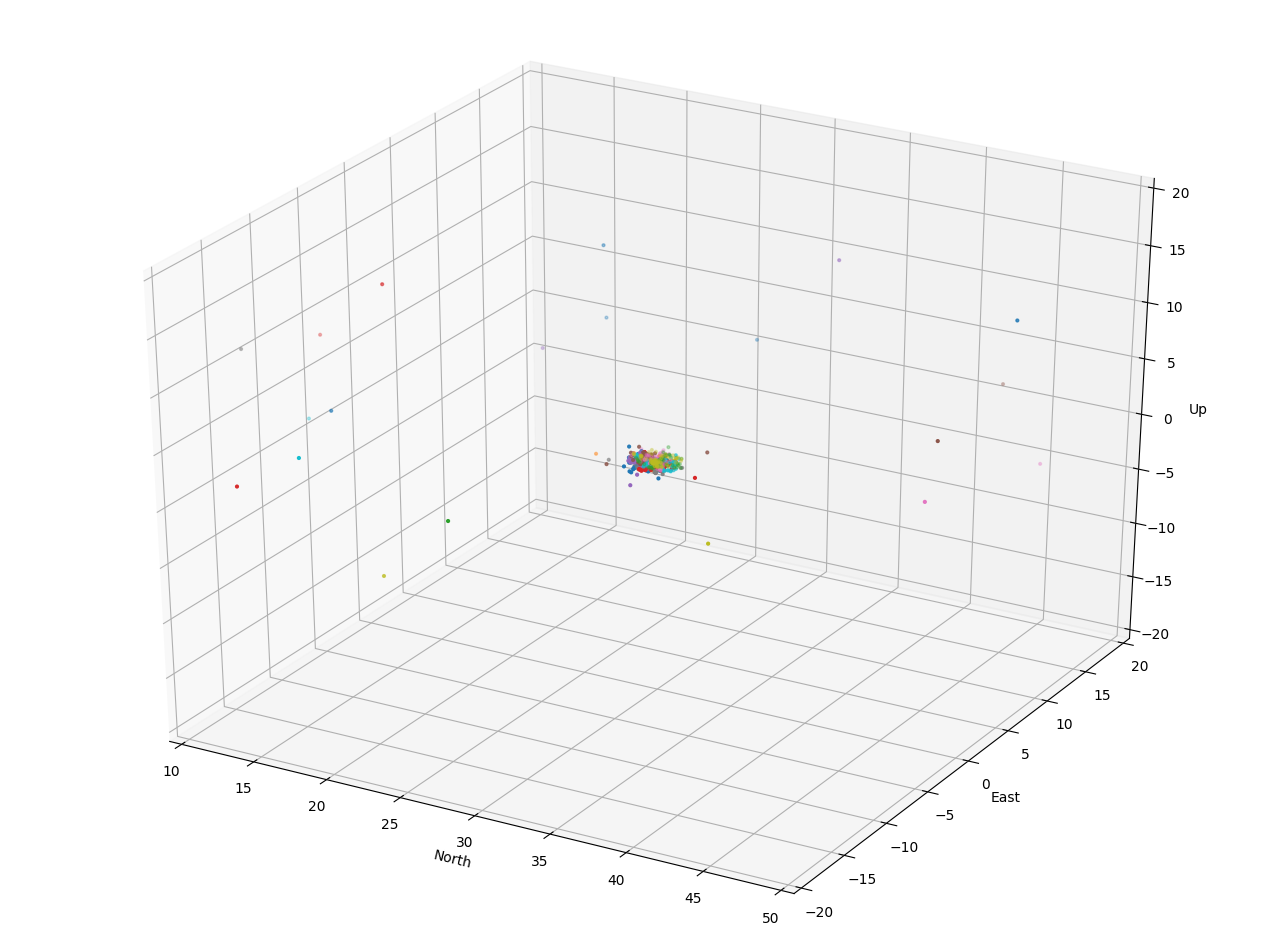
\includegraphics[width=0.9\textwidth]{images/whycon_pose_estimation_with_outliers.png}
%     \caption{WhyCon stationary pose estimation with outliers included.}
%     \label{fig:whycon_stationary_pose_estimation_with_outliers}
% \end{figure}

Figure \ref{fig:whycon_stationary_error} shows a graph of the magnitude of the 3-dimensional WhyCon pose estimate error over the course of 10 approaches. That is, if the error $e$ of the estimate has components $e_x,e_y,e_z$, the plotted value for the magnitude of this error is simply $|e|=\sqrt{e_x^2+e_y^2+e_z^2}$: the Euclidean distance between the true value and estimated value of the position of the WhyCon marker. These results generally show an increase in pose estimation error when the distance from the marker increases. A regression line following Equation \ref{equation:whycon_error_regression} estimates the relationship between the WhyCon pose estimation error and the distance to the WhyCon marker, where $y$ denotes the pose estimation error and $x$ denotes the distance to the marker. The standard error for this regression is $\sigma=0.0154$ over the $n=1292$ samples. The main takeaway from this result is that the WhyCon marker can be used from a distance of about 1 meter to a distance of about 18 meters. When the drone is closer than 1 meter to the landing platform, the WhyCon marker is out of the camera's field of view, and when the drone is sufficiently far away from the landing platform, the marker is simply not recognizable. 

\begin{equation}
    y=-0.004x^3+0.180x^2-0.876x+1.843
    \label{equation:whycon_error_regression}
\end{equation}

\begin{figure}[ht]
    \centering
    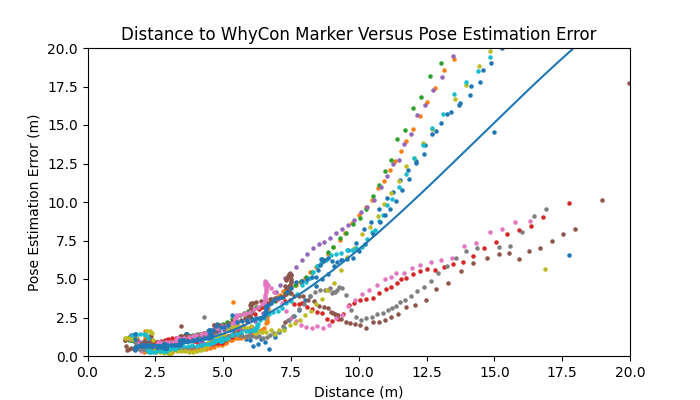
\includegraphics[width=0.65\textwidth]{images/whycon_pose_estimation_error.png}
    \caption{Distance to WhyCon marker vs. magnitude of 3-dimensional pose estimate error.}
    \label{fig:whycon_stationary_error}
\end{figure}



\subsection{WhyCode Trials}
\label{subsection:whycode_trials}

% {\color{red}This section ``WhyCode Trials'' will provide an explanation for the attempt made to use WhyCode and the reasons why it failed in this scenario. WhyCode markers are preferable to WhyCon markers because, in theory, they can provide unambiguous yaw orientation unlike WhyCon markers. However, in each set of WhyCode markers (sets are grouped by the number of bits contained in their IDs), there are necessarily markers that are rotationally equivalent to each other, but with different IDs. The current implementation of \texttt{whycon\_ros} is able to identify the ID of whichever WhyCode marker it sees, but it may determine the ID of a rotationally symmetric marker instead of the intended marker. A workaround for this was attempted: 2-bit WhyCode markers with ID 1 and 2 are rotationally symmetric, but have two distinct sides, so that if ID 1 is recognized, then the orientation could theoretically be used without modification, and if ID 2 is recognized, then the orientation could be flipped by $\pi$ radians in the axis normal to the marker. The GUI even unambiguously identifies the yaw of the marker, but the orientation of the marker in the published ROS topic changes unpredictably (by $\pi$ radians in the marker's z-axis, without a change in the marker's recognized ID), which causes non-negligible issues in the pose estimation. This route is still worth pursuing because of the simpler and more robust algorithm used in recognizing WhyCon/WhyCode markers. A WhyCode marker could replace the AprilTag marker that is used for final descent.}

The original landing platform design was a single WhyCode marker. This minimalistic design could simplify the system by lessening the amount of coordinate system transforms and components within the gimbal controller, as well as the physical landing platform itself. However, due to two issues, this option was abandoned in favor of the aforementioned landing platform design.

The first issue is that each set of WhyCode markers (where a group is defined by the number of bits contained in the group's IDs) contains rotationally symmetric markers. This is true for markers with more than a single ID bit. This is shown in Figure \ref{fig:whycode_rotational_symmetry}, where the number of ID bits is 2. Moreover, markers such as those with IDs 3 and 4 do not provide an unambiguous orientation, as there is no way to define a unique ``front'' on the marker. However, the markers with IDs 1 and 2, though rotationally equivalent to each other, do have a potential ``front'' which would allow for the unambiguous determination of the marker's yaw. The original plan for the system design involved placing the ``front'' of the marker at the center of the larger white semi-circle of a WhyCode marker with ID 1. The anticipated workaround for the problem of the marker's rotational symmetry was to use the natural orientation of the marker if the \texttt{whycon\_ros} system recognized its ID as 1, and to apply an initial rotation of $\pi$ radians about the marker's central z axis if it was recognized with an ID of 2. In theory this method should still work, but it was never fully attempted because of the second issue.

\begin{figure}[ht]
    \begin{subfigure}[b]{0.23\textwidth}
        \centering
        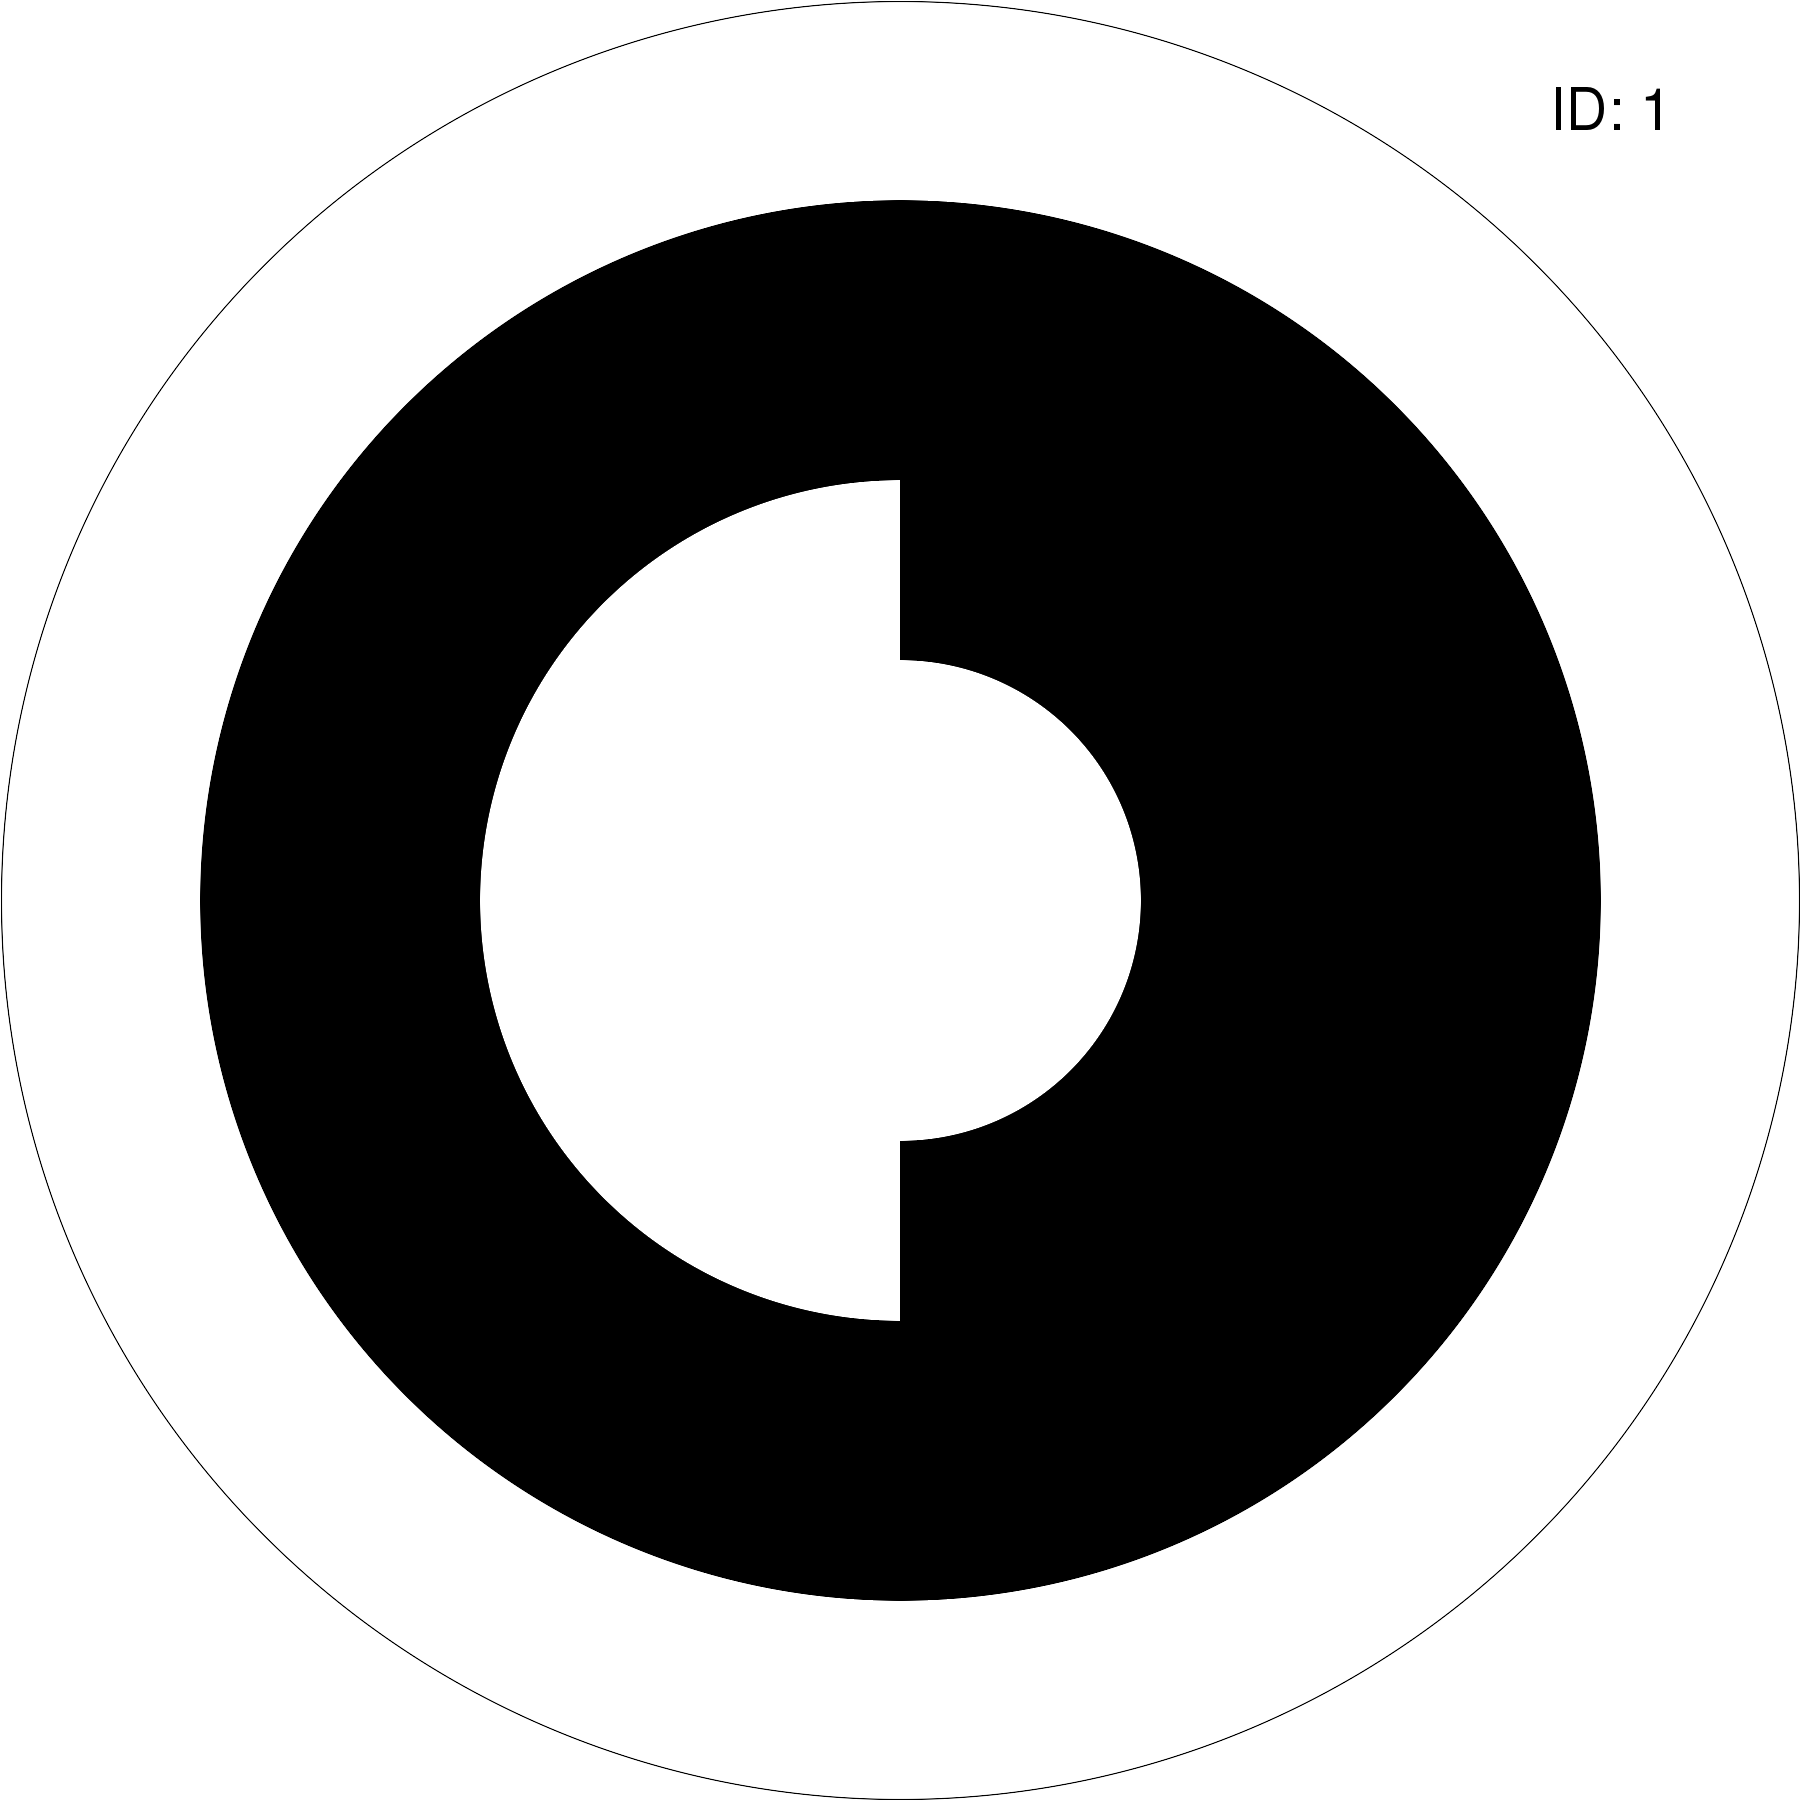
\includegraphics[width=\textwidth]{images/00000001.png}
        % \caption{``Chessboard'' detection.}
        \label{subfig:whycode_1}
    \end{subfigure}
    \begin{subfigure}[b]{0.23\textwidth}
        \centering
        \includegraphics[width=\textwidth]{images/00000002.png}
        % \caption{``Chessboard'' detection.}
        \label{subfig:whycode_2}
    \end{subfigure}
    \begin{subfigure}[b]{0.23\textwidth}
        \centering
        \includegraphics[width=\textwidth]{images/00000003.png}
        % \caption{``Chessboard'' detection.}
        \label{subfig:whycode_3}
    \end{subfigure}
    \begin{subfigure}[b]{0.23\textwidth}
        \centering
        \includegraphics[width=\textwidth]{images/00000004.png}
        % \caption{``Chessboard'' detection.}
        \label{subfig:whycode_4}
    \end{subfigure}
    \caption{Rotationally symmetric WhyCode markers with 2 ID bits, generated from the LCAS \texttt{whycode\_id\_gen}.}
    \label{fig:whycode_rotational_symmetry}
\end{figure}

The second issue with using WhyCode markers came from the unanticipated, destructive interaction between the PID systems used to aim the camera, and the WhyCode system. The exact cause of the issue has not been determined, but it corresponds to sign changes in the positional components of the WhyCode marker's pose. This issue only happens specifically when the marker is being identified, and it does not happen every time the marker is identified. This made the issue very hard to isolate. Further investigation into this issue is necessary.

The issue can be illustrated through an experiment, the results of which are shown in Figures \ref{subfig:whycode_camera_position} and \ref{subfig:whycode_camera_orientation}, where the drone was stationary on the ground, viewing a marker in front of it, with the gimbal controller aiming the camera at the marker. As shown in Figure \ref{subfig:whycode_camera_position}, the x and y components of the marker within the camera frame are close to 0, but oscillate, after the marker is detected. This oscillation is to be expected because of the nature of PID controllers, and it is not inherently a problem in itself. However, the orientation of the marker is an important component of the pose, and, as Figure \ref{subfig:whycode_camera_orientation} shows, the small, acceptable oscillation in the positional components corresponds to large, unacceptable oscillation in the marker's recognized orientation. The oscillation in the orientation does not represent noise, but rather an axial flip without a change in the perceived marker ID. The ultimate result of this was that the marker's pose could not be reliably determined while the WhyCon module's identification functionality was running. Because of this issue, the identified WhyCode markers were temporarily abandoned in favor of the April Tag markers for the determination of the landing platform's yaw.

\begin{figure}
    \centering
        \includegraphics[width=0.8\textwidth]{images/whycode_camera_pose_constrained.png}
        \caption{$x$ and $y$ position components of the WhyCode marker's pose in the camera frame.}
        \label{subfig:whycode_camera_position}
\end{figure}

\begin{figure}
    \centering
        \includegraphics[width=0.7\textwidth]{images/whycode_camera_orientation_constrained.png}
        \caption{$x,y,z,w$ orientation components of the WhyCode marker's pose in the camera frame.}
        \label{subfig:whycode_camera_orientation}
\end{figure}

% \begin{figure}[ht]
%     \centering
%     \begin{subfigure}[b]{0.47\textwidth}
%         \centering
%         \includegraphics[width=\textwidth]{images/whycode_camera_pose_constrained.png}
%         \caption{$x$ and $y$ position components of the WhyCode marker's pose in the camera frame.}
%         \label{subfig:whycode_camera_position}
%     \end{subfigure}
%     \begin{subfigure}[b]{0.47\textwidth}
%         \centering
%         \includegraphics[width=\textwidth]{images/whycode_camera_orientation_constrained.png}
%         \caption{$x,y,z,w$ orientation components of the WhyCode marker's pose in the camera frame.}
%         \label{subfig:whycode_camera_orientation}
%     \end{subfigure}
%     \caption[Destructive interaction between WhyCode system and gimbal controller.]{Destructive interaction between the WhyCode system and gimbal PID controllers, resulting from \gls{PID} oscillation.}
%     \label{subfig:whycode_problems}
% \end{figure}

\begin{figure}[h!]
    \centering
    \includegraphics[width=0.5\textwidth]{images/whycode_camera_orientation_constrained_corrected.png}
    \caption[WhyCode marker orientation components after ``fixing.'']{WhyCode marker orientation components after ``fixing.'' This shows that the persistent flipping shown in Figure \ref{subfig:whycode_camera_orientation} has been removed, and the perceived orientation of the WhyCode marker is stable.}
    \label{fig:whycode_problems_corrected}
\end{figure}

A simple, ``bandaid'' method for dealing with the WhyCode orientation problem shown in Figures \ref{subfig:whycode_camera_orientation} and \ref{subfig:whycode_camera_position} has been implemented. Let $i$ represent the index of a detection, and let be a quaternion (Explained in Section \ref{subsection:quaternions}) representing $d_i$ representing the $i\mathrm{th}$ detected orientation. At detection $i$, the gimbal controller stores the orientation, $d_i$, of the marker. It compares the \textit{inverse} of the detected orientation at frame $i+1$, $d_{i+1}^{-1}$ to the orientation of the marker at detection $i+1$. If the angle represented by $d_{i+1}^{-1}$ is within some small angular displacement $\theta_d$ from the angle represented by $d_i$, then the inverse is assumed to be the correct orientation, is used for further calculation, and is stored for comparison at detection $i+2$. Figure \ref{fig:whycode_problems_corrected} shows how this method maintains continuity within the same test shown in Figure \ref{subfig:whycode_camera_orientation}, when $\theta_d=2\degree$. It is somewhat difficult to identify the cause of this error within the WhyCode source, so as a proof of concept, this ``bandaid'' method was used to correct the issue in this particular scenario. While the fix corrects the orientation of the marker in this particular scenario, it did not solve the issue in testing generally.

\section{April Tag Pose Estimation}

Similar experiments to those used to test WhyCon pose estimation were carried out for the April Tag markers. Figure \ref{fig:apriltag_pose_estimation} shows the wide spread of high-error pose estimation for the April Tag over the course of 10 approaches. It is not surprising that the marker of size 0.3125 meters by 0.3125 meters is not accurately located from the same distance as the WhyCon marker. However, since the April Tag marker is only to be used in late descent, this can be overlooked in favor of the marker's performance at lower altitudes. Table \ref{tab:stationary_apriltag_pose_estimation} outlines the performance of April Tag pose estimation during 10 approaches at altitudes between 0 and 10 meters. The standard deviations of the measurements decrease as distance from the marker decreases, while the means remain in the same acceptable region. Similarly to WhyCon, the z component of the April Tag's pose is somewhat incorrectly estimated - but not prohibitively so. 

\begin{figure}[ht]
    \centering
    \includegraphics[width=0.85\textwidth]{images/apriltag_pose_estimation.png}
    \caption{April Tag pose estimation.}
    \label{fig:apriltag_pose_estimation}
\end{figure}

\begin{table}[h]
    \centering
    \begin{tabular}{|c|r|}
    \hline
        $\mu_x$ &       0.0720\\\hline
        $\mu_y$ &       30.060\\\hline
        $\mu_z$ &       -0.394\\\hline
        $\sigma_x$ &    1.230\\\hline
        $\sigma_y$ &    1.297\\\hline
        $\sigma_z$ &    0.589\\\hline
        $n$ & 2707\\\hline
    \end{tabular}
    \caption{Means and standard variations for April Tag estimation.}
    \label{tab:stationary_apriltag_pose_estimation}
\end{table}

The pose estimation is visualized in Figure \ref{fig:apriltag_pose_estimation}. The pose was estimated at altitudes varying from 0 to 10 meters in motion, revealing an exponential relationship between the distance from the marker and error in pose estimation magnitude as shown in Figure \ref{fig:apriltag_pose_estimation_error}. The main takeaway from this test is that the error in pose estimation increases with the distance from the marker to the drone, but at close distances the pose estimate is very accurate. Furthermore, the pose estimate is useful to the system throughout the approaches, even in spite of its error. A regression following Equation \ref{equation:april_tag_regression} describes the an estimate of the relationship between the pose estimation error and the distance to the marker, where $y$ denotes the error and $x$ denotes the distance to the marker. The standard error for this regression is $\sigma = 0.0047$ meters over the samples.%, with $n=2707$ samples.

\begin{equation}
    y = -0.002x^3+0.098x^2-0.095x+0.256
    \label{equation:april_tag_regression}
\end{equation}

\begin{figure}[h!]
    \centering
    \includegraphics[width=0.65\textwidth]{images/apriltag_pose_estimation_error.png}
    \caption{Pose estimation error versus distance for the April Tag marker.}
    \label{fig:apriltag_pose_estimation_error}
\end{figure}

% The exponential regression generated for this graph shows that the error in pose estimation for the April Tag marker roughly follows the exponential curve described by Equation \ref{equation:apriltag_pose_estimation_error_regression}, where $x$ denotes the Euclidean distance in meters from the drone to the landing platform and $y$ denotes the error in pose estimation in meters. The coefficient of determination is $r^2 = 0.84$, showing that the fit is somewhat loose. This is likely because of the varying and complex motion that the April Tag marker takes in the camera's field of view even during the later portions of approach and landing.

% \begin{equation}
%     y = e^{0.342x - 1.472}
%     \label{equation:apriltag_pose_estimation_error_regression}
% \end{equation}

\subsection{Yaw Estimation}

The yaw of the April Tag is a necessary data point during autonomous landing, as the drone must align itself to the landing pad in order to guarantee that a fiducial marker (in this case, the April Tag) will be in its field of view during the final part of the landing sequence. Thus, the performance of the April Tag's yaw recognition is evaluated. Figure \ref{fig:apriltag_yaw_estimation} shows the perceived yaw angle during the 10 test approaches, and Table \ref{tab:apriltag_yaw_stats} describes them statistically. 


\begin{figure}[h]
    \centering
    \includegraphics[width=0.65\textwidth]{images/apriltag_yaw_estimation.png}
    \caption{Estimation of the April Tag marker's yaw during the pose estimation approaches.}
    \label{fig:apriltag_yaw_estimation}
\end{figure}

\vspace{-0.25cm}
\begin{table}[ht]
    \centering
    \begin{tabular}{|c|r|}
    \hline
        $\mu_{yaw}$  & 3.149 \\\hline
        $\sigma_{yaw}$ & 0.044 \\\hline
    \end{tabular}
    \caption{}
    \label{tab:apriltag_yaw_stats}
\end{table}

\vspace{-0.25cm}
These show that the yaw estimation of the April Tag marker is quite accurate over its detection range. An angle of $\frac{\pi}{2}$ radians represents due north, however the April Tag marker has been rotated by an additional $\frac{\pi}{2}$ radians in its position on the landing platform, giving the estimated yaw of $3.149 \approx \pi$ radians. Figure \ref{fig:apriltag_yaw_estimation_error} shows the absolute value of the April Tag's yaw estimation error. It is apparent that the yaw estimation error has increases when the distance from the landing platform is both very high and very low. A regression following Equation \ref{equation:apriltag_yaw_error_regression} describes the relationship between the yaw estimation error and the distance to the April Tag marker, with $y$ denoting the yaw estimation error in radians and $x$ denoting the distance to the marker in meters. The standard error of the regression is $\sigma=0.0306$ radians over the $n=2707$ samples.

\begin{equation}
    y=0.003x^2-0.018x+0.051
    \label{equation:apriltag_yaw_error_regression}
\end{equation}

% \vspace{-0.25cm}
\begin{figure}[h!]
    \centering
    \includegraphics[width=0.65\textwidth]{images/apriltag_yaw_estimation_error.png}
    \caption{April Tag yaw estimation error with regression.}
    \label{fig:apriltag_yaw_estimation_error}
\end{figure}

The variance of the error in the April Tag's yaw estimation increases at very close distances. This is likely caused by the high angle of deflection of the marker in the camera's field of view, as shown by Figure \ref{fig:apriltag_landed_view}. However, this small issue can be overcome easily with the landing policy. The yaw position is locked if the yaw displacement of the drone is less than 5 degrees, or approximately 0.0873 radians, meaning that small variations in the yaw measurement will have no effect on the drone's behavior.

\begin{figure}[h]
    \centering
    \includegraphics[width=0.5\textwidth]{images/landed_view.png}
    \caption{The view from the drone immediately after landing, with the April Tag's high angle of deflection.}
    \label{fig:apriltag_landed_view}
\end{figure}

% \section{\color{red}Landing Pad Pose Estimate Visualization}

% {\color{red}Here I will discuss an attempt to add a visualization for the landing pad pose estimate in Gazebo, the difficulties in using it, and why it was eventually abandoned.}


% \vspace{100cm}
\section{Initial PID Controller Tuning}
\label{subsection:pid_tuning}

% {\color{red}Here I will describe the process of tuning the velocity PID controllers. The intuitive way to describe it is that the distance at which the system changes from P to PD controllers, and the derivative gain were set to eliminate overshoot while minimizing the error over time. I still do not know exactly how to quantify this.}

PID controllers have parameters which must be tuned for the system and conditions that they will face. The first step in landing on a stationary platform is to tune these parameters using a priori knowledge of PID controller behavior and simple trial and error. Importantly, in a scenario involving a stationary landing platform with stable, well-tuned PID controllers, all of the state errors will converge to 0. This means that the integral gain of each of the PID controllers can be left at 0, making the control purely PD-based. This is conceptually different from a scenario wherein the landing pad is moving, which requires the additional integral gain (described in Section \ref{section:moving_landing_scenarios}). The approach taken in this project is to first tune the PID systems for a stable landing on a stationary landing platform, and then transition to moving landing scenarios, tuning only the integral gain.

\subsection{North and East Velocity Controllers}

The goals in tuning the gains of the east and north velocity PID controllers in order of priority are as follows:
\begin{enumerate}
    \item \textbf{Avoid overshoot.} Overshooting the landing platform causes complications in aiming the camera and increases both time and energy spent in landing.
    \item \textbf{Avoid undershoot.} Undershooting the landing platform increases the time and energy spent in landing. Avoiding overshoot takes precedence over avoiding undershoot. Overshoot is eliminated first. If this causes undershoot then the undershoot is gradually eliminated as long as it does not cause overshoot.
    \item \textbf{Minimize energy required for landing.} The energy required for landing must comprise only a small portion of the battery's capacity in order to maximize usable flight time for mission tasks. This metric is obviously related to the time spent for landing, but differs in that it accounts for energy-intensive maneuvers such as course correction.
    \item \textbf{Minimize time required for landing.} As the landing time increases, so does the possibility changes in the environment and the energy required for the landing.
\end{enumerate}

Initial, informal experiments showed that PID parameters shown in Table \ref{tab:initial_parameters} provided an imperfect but relatively reliable performance in the drone's approach towards the landing pad. These initial experiments decrease the search space for the PID parameters and therefore decrease the time for testing PID gains more rigorously. The parameters are all negative because the PID controllers in this scenario are reverse-acting - that is, a positive change in the control effort produces a negative change in the error between the set point and the state variable. Phase 1 refers to the PID gains used upon initial recognition of the landing platform. Phase 2 refers to the PID gains used when the drone is displaced by an intermediate distance from the landing platform. Phase 3 refers to the PID gains used when the drone is in its final approach.

\begin{table}[ht]
    \centering
    \begin{tabular}{|c|c|c|c|}
    \hline
        Phase & $k_p$ & $p_i$ & $k_d$ \\\hline
        1 & -0.7 & -0.0 & -0.4 \\\hline
        2 & -0.4 & -0.0 & -0.7 \\\hline
        3 & -0.3 & -0.0 & -0.9 \\\hline
    \end{tabular}
    \caption{Initial north and east PID tuning parameters. The same parameters are used for both systems.}
    \label{tab:initial_parameters}
\end{table}

The search space for the north and east PID parameters is comprised of all combinations of $k_p \pm 0.1$ and $k_d \pm 0.1$ for phases 1 and 2. The gains for phase 3 are kept constant in order to save time during the slow testing in Gazebo. Each of the combinations of gains is tested over 5 approaches. The approach series starts at the origin with an altitude of 10 meters, with the drone facing directly south in order to ensure that the landing platform is not in the drone's field of view. The landing controller is initially disabled by sending a PWM signal of 1100$\mu s$ on RC channel 11. Then, the drone is sent to a point 200 meters directly north of its original position, while also facing directly north. At this point, the landing controller is enabled by sending a PWM signal of 1900 $\mu s$ on RC channel 11. With each approach, the drone's starting position is moved 1 meter to the right in order to have variation in both planar dimensions of the drone's displacement from the landing pad. When the landing pad, positioned at 30 meters north of the origin, comes into the drone's field of view, the landing controller's north and east velocity PID controllers begin to control the drone. An approach is considered successful if the drone maintains a planar distance of no more than 1.6 meters from the landing pad (calculated through pose estimation) for 3 consecutive seconds. The system is given a maximum of 45 seconds from the acquisition of the landing platform to achieve a success before the approach is considered a failure. After a success or failure, the landing system is disabled, the drone is positioned at the starting point of the next approach, and the test is started again. For consistency, this process is automated using a Python script \texttt{control\_pid\_ne.py}. In this way, the drone follows exactly the same initial trajectory with the same velocity before acquisition of the landing platform. During these tests, the yaw correction and altitude correction of the landing system are inhibited to isolate the performance of the north and east PID controllers exclusively.

During each approach, the Python script records the time and energy required by the drone from the point of visual acquisition of the landing platform to a success or failure. The value for time is the ROS simulation time. The value for the energy is taken from the \texttt{battery\_status} MAVlink message 147. This message provides a value in \gls{hJ} given a properly calibrated power module onboard the drone. The gain combinations are rated according to the average time and energy required over the course of the 5 approaches. The 81 gain combinations are described by 405 separate approaches, but the results of the best combinations are shown in Table \ref{tab:initial_ne_gains}.

\begin{table}[h]
    \centering
    \begin{tabular}{|c|c|c|c|c|c|c|c|c|c|c|}
    	\hline $k_{p1}$ & $k_{i1}$ & $k_{d1}$ & $k_{p2}$ & $k_{i2}$ & $k_{d2}$ & $k_{p3}$ & $k_{i3}$ & $k_{d3}$ & $t_{ave}$ (s) & $e_{ave}$ (hJ) \\\hline
    	-0.7 & -0.0 & -0.4 & -0.3 & -0.0 & -0.7 & -0.3 & -0.0 & -0.8 & 13.0 & 52.4 \\\hline
    	-0.7 & -0.0 & -0.4 & -0.3 & -0.0 & -0.7 & -0.3 & -0.0 & -0.9 & 13.7 & 54.8 \\\hline
    	-0.7 & -0.0 & -0.4 & -0.3 & -0.0 & -0.8 & -0.3 & -0.0 & -0.9 & 13.8 & 55.4 \\\hline
    	-0.7 & -0.0 & -0.4 & -0.3 & -0.0 & -0.8 & -0.3 & -0.0 & -1.0 & 13.9 & 55.2 \\\hline
    	-0.7 & -0.0 & -0.4 & -0.3 & -0.0 & -0.8 & -0.2 & -0.0 & -0.8 & 15.0 & 60.0 \\\hline
    \end{tabular}
    \caption{Best 5 initial gain combinations by time and energy for the north and east PID controllers}
    \label{tab:initial_ne_gains}
\end{table}

\begin{figure}[ht]
    \centering
    % \includegraphics[width=0.45\textwidth]{images/best_initial_ne_pid_gains.png}
    % \caption{Caption}
    % \label{fig:my_label}
    \begin{subfigure}[b]{0.45\textwidth}
        \centering
        \includegraphics[width=\textwidth]{images/best_initial_ne_pid_gains.png}
        \caption{Best-performing N/E PID parameters.}
        \label{subfig:best_initial_pid_tuning}
    \end{subfigure}
    \begin{subfigure}[b]{0.45\textwidth}
        \centering
        \includegraphics[width=\textwidth]{images/bad_ne_pid_tuning.png}
        \caption{Badly-performing N/E PID parameters.}
        \label{subfig:bad_initial_pid_tuning}
    \end{subfigure}
    \caption{Interesting initial north and east PID performances.}
    \label{fig:initial_ne_pid_gains}
\end{figure}

The graph of the best initial north and east PID gains is shown in Figure \ref{subfig:best_initial_pid_tuning}. The time plotted is the time \textit{before} a success or failure, so time $t=0$ indicates the point at which the drone's planar position has been sufficiently close to the landing platform's planar position for 3 seconds. The distance plotted is the difference in the planar positions of the drone and the landing pad. The perceived distance to the landing pad steadily and predictably decreases without salient local minima or maxima, which indicates that there is no positional overshoot. On the other hand, Figure \ref{subfig:bad_initial_pid_tuning} shows the performance of badly-performing PID parameters. Of the 5 approach attempts, only 3 were successful within the 45-second time limit, even with initial conditions which were negligibly different from those in Figure \ref{subfig:best_initial_pid_tuning}. Moreover, the salient local minima and maxima in the perceived distances shows that the drone approached the landing pad quickly, but overshot the target position and had to backtrack, which significantly increased the time and energy required for the approach. It is also important to note that these gains pertain to the most ideal scenario of landing on a stationary landing pad with no wind or other external factors.

Figure \ref{fig:initial_ne_pid_gains} additionally shows that the initial distance estimates (and inherently the initial pose estimates) of the drone relative to the landing platform are inaccurate. This means that the landing pad - the WhyCon marker in particular, since it is identified first - can be recognized in the drone's field of view before the pose can be accurately determined. This can be seen in all of the depicted approaches (and indeed in all of the test results) via the phenomenon that the initial distance estimate of about 10 meters, when the landing pad is just barely identifiable, jumps to about 18 meters when it becomes \textit{properly} identifiable. A number of factors are at play in causing this: namely the relatively small pixel area of the WhyCon marker within the drone's field of view, the angular displacement between the camera and the landing pad, and the motion of the camera as the gimbal controller attempts to aim the camera at the landing pad. A key aspect of the success of these tests is that the drone is moving towards the landing platform at the point when it is initially identified. This allows the pose estimation accuracy - and inherently the distance estimation accuracy - to increase over time.

\subsection{Up Velocity Controller}

The ``up'' PID controller is used to control the downward velocity of the drone during descent towards the landing platform. It is oriented upwards instead of downwards in order to conform to the typical east-north-up coordinate system orientation that is used in MAVROS and ArduPilot. As in the initial tuning for the north and east velocity PID controllers, the main goals in setting the initial gains for the velocity PID controller in the ``up'' direction are to prevent overshoot, prevent undershoot, and minimize time and energy spent. The most important of these goals is to prevent overshoot, as overshoot in this scenario means hitting the landing pad at higher than expected velocity.

Similarly to the north and east PID testing, the process of testing the up PID was automated by a Python script \texttt{control\_pid\_u.py}. The landing platform was positioned 30 meters directly north of the origin, and the drone was positioned directly above the landing platform at an altitude of 10 meters with the camera aimed directly at the landing platform and the landing controller disabled. At the point when the landing controller is enabled, a single test is considered to have begun, and the Python script records the position and velocity of the drone throughout the landing until the motors are disarmed. This is repeated for several sets of PD gains. The integral gain is not necessary here because the drone is not affected by persistent non-zero error in this dimension. The tests are repeated for all combinations of $k_p$ and $k_d$, where $k_p \in \{ 0.6, 0.7, 0.8, 0.9 \}$ and $k_d \in \{  0.4, 0.5, 0.6, 0.7 \}$. Each combination of gains is tested 5 times, giving a total of 80 runs. During these tests, the base descent radius is increased to 30 centimeters in order to avoid extraneous energy and time expenditure resulting from unavoidable drift in the drone's east and north positions. The best 5 gain combinations are shown in Table \ref{tab:up_pid_gains}.

\begin{table}[ht]
    \centering
    \begin{tabular}{|c|c|c|c|c|}
    	\hline $k_{p}$ & $k_{i}$ & $k_{d}$ & $t_{ave}$ (s) & $e_{ave}$ (hJ) \\\hline
    	-0.9 & -0.0 & -0.5 & 13.8 & 53.6 \\\hline
    	-0.8 & -0.0 & -0.4 & 13.8 & 54.0 \\\hline
    	-0.8 & -0.0 & -0.5 & 14.3 & 56.2 \\\hline
    	-0.9 & -0.0 & -0.7 & 14.4 & 56.0 \\\hline
    	-0.7 & -0.0 & -0.4 & 14.6 & 57.0 \\\hline
    \end{tabular}
    \caption{Best gain combinations for up velocity PID controller.}
    \label{tab:up_pid_gains}
\end{table}

Over the 80 tests, the average landing time for each combination is only in the range of $\left[ 13.8s, 19.7s \right]$, with a mean of $\mu_t = 16.06s$ and standard deviation of $\sigma_t = 3.14s$. The corresponding values for the energy expended are in the range $\left[ 53.6 \mathrm{hJ}, 73.4 \mathrm{hJ} \right]$, with mean $\mu_e = 61.75 \mathrm{hJ}$ and standard deviation $\sigma_e = 8.33 \mathrm{hJ}$. This means that the performances of all tested gain combinations are fairly similar, however the gains $k_p=-09, k_i=-0.0, k_d=-0.5$ are chosen according to the aforementioned goals. The performance of the best combination of gains is shown in Figure \ref{fig:best_u_pid_gains}.

\begin{figure}[ht]
    \centering
    \begin{subfigure}[b]{0.49\textwidth}
        \centering
        \includegraphics[width=\textwidth]{images/best_pid_u_altitude.png}
        \caption{Perceived altitude vs. time before landing.}
        \label{subfig:best_initial_pid_u_altitude}
    \end{subfigure}
    \begin{subfigure}[b]{0.49\textwidth}
        \centering
        \includegraphics[width=\textwidth]{images/best_pid_u_velocity.png}
        \caption{Vertical velocity vs. time before landing.}
        \label{subfig:best_initial_pid_u_velocity}
    \end{subfigure}
    \caption{Visualization of best U PID gain performance.}
    \label{fig:best_u_pid_gains}
\end{figure}

Figure \ref{subfig:best_initial_pid_u_altitude} shows the near-linear descent of the drone towards the landing platform in the early part of the landing, with a gradual slowdown as the drone gets closer and closer to touchdown. Figure \ref{subfig:best_initial_pid_u_velocity} shows the same phenomenon in terms of velocity. The magnitude of the velocity increases suddenly after the landing controller is enabled, then remains relatively constant until the derivative component of the PID system slows the velocity to 0.

\subsection{Yaw Velocity Controller}

The gains for the yaw velocity controller were determined experimentally through tests similar to those for the other PID controllers. Specifically, the test is automated using a Python script \texttt{control\_yaw\_testing.py}. First, the drone is positioned directly above the landing pad at an altitude of 10 meters. With the landing controller disabled, the drone rotates to 10 different initial angles which are equally placed in the interval $\theta_{initial} \in [0, 2\pi)$. The landing controller is then enabled, with the linear velocity set points always equal to 0, in order to isolate the behavior of the yaw PID controller. The time and yaw displacement are recorded for 10 seconds. The process is repeated at the same location for the remaining initial angles. The entire process is then repeated for multiple positions.

Since the Iris model has very accurate control over its yaw position and velocity, the yaw velocity PID controller performs very well. The results are illustrated in Figure \ref{fig:initial_yaw_tuning}.

\begin{figure}[ht]
    \centering
    \begin{subfigure}[b]{0.45\textwidth}
        \centering
        \includegraphics[width=\textwidth]{images/yaw_pid_testing_east_0.png}
        \caption{Yaw correction with drone directly above landing pad at altitude of 10 meters.}
        \label{subfig:yaw_pid_testing_east_0}
    \end{subfigure}
    \begin{subfigure}[b]{0.45\textwidth}
        \centering
        \includegraphics[width=\textwidth]{images/yaw_pid_testing_east_2.png}
        \caption{Yaw correction with drone 2 meters east of landing platform at altitude of 7 meters.}
        \label{subfig:yaw_pid_testing_east_2}
    \end{subfigure}
    \caption{Visualization of velocity yaw controller performance.}
    \label{fig:initial_yaw_tuning}
\end{figure}

\section{Stationary Landing Scenarios}
\label{subsection:stationary_landing_scenarios}

The first test of the landing system in its entirety is a series of 5 landing sequences starting with the drone at the origin and the landing platform 30 meters directly north of the origin. These are essentially a repeat of the test for the north and east velocity PID systems, but with the up and yaw PID systems active. The results for the initial gains are visualized in Figure \ref{subfig:linear_land_test_initial}. After initial descent, it is easy to see a sharp inflection point representing positional overshoot overshoot. Although the parameters do allow the system to land successfully, the overshoot is not ideal. The system parameters were re-tuned manually over the course of several experiments. The descent region was slightly enlarged, giving the drone more area to continue its descent without stopping, and causing earlier PID reconfiguration. The derivative gain $k_d$ was increased in phases 2 and 3 in order to slow the drone more drastically. The proportional gain was decreased in phase 2, also to slow the drone's approach. The resulting, smoother performance is shown in Figure \ref{subfig:linear_land_test_better}, and the performances are compared in Table \ref{tab:linear_land_performance_comparison}.

\begin{figure}[ht]
    \centering
    \begin{subfigure}[b]{0.45\textwidth}
        \centering
        \includegraphics[width=\textwidth]{images/linear_land_test_initial.png}
        \caption{Initial parameters (positional overshoot).}
        \label{subfig:linear_land_test_initial}
    \end{subfigure}
    \begin{subfigure}[b]{0.45\textwidth}
        \centering
        \includegraphics[width=\textwidth]{images/linear_land_test_better.png}
        \caption{Looser, more efficient parameters.}
        \label{subfig:linear_land_test_better}
    \end{subfigure}
    \caption{Comparison of initial parameters versus manually-tuned parameters.}
    \label{fig:initial_u_pid_gains}
\end{figure}

\begin{table}[ht]
    \centering
    \resizebox{\textwidth}{!}
    { 
    \begin{tabular}{|c|c|c|c|c|c|c|c|c|c|c|c|c|c|}
    \cline{2-14}
    	\multicolumn{1}{c|}{} & $k_{p1}$ & $k_{i1}$ & $k_{d1}$ & $k_{p2}$ & $k_{i2}$ & $k_{d2}$ & $k_{p3}$ & $k_{i3}$ & $k_{d3}$ & $\mu_t$ (s) & $\sigma_t$ (s) & $\mu_e$ (hJ) & $\sigma_e$ (hJ) \\\hline
    	Initial & -0.7 & -0.0 & -0.4 & -0.3 & -0.0 & -0.7 & -0.3 & -0.0 & -0.8 & 39.8 & 0.65 & 130.0 & 2.1 \\\hline
    	Improved & -0.7 & -0.0 & -0.4 & -0.3 & -0.0 & -0.8 & -0.3 & -0.0 & -0.9 & 35.6 & 1.8 & 112.8 & 7.5 \\\hline
    \end{tabular}
    }
    \caption{Comparison of initial and manually-tuned gains and performances during 5 linear landing tests.}
    \label{tab:linear_land_performance_comparison}
\end{table}

Figure \ref{subfig:radial_land_test_initial} represents the landing trajectories taken by the drone over a series of 10 landings from various angles around the landing platform using the initially-determined PID gains and system parameters. Gazebo provides the coordinates of the Iris model via a ROS topic and these are used as a true value for the position of the drone. The landing pad is positioned at $(x,y,z)=(0,30,0)$ in the ENU coordinate frame starting at the origin of \texttt{sandbox.world}. For clarity, the plotted trajectories begin at the moment that the drone first detects the landing pad and continue until the drone has landed. The approaches begin at a height of 10 meters. A Python script places the drone initially in 10 equidistant starting points which are positioned around the landing pad at a radius of 30 meters. The landing controller is then enabled and the drone is sent towards the landing pad. Upon detection of the landing pad, the landing controller takes control of the drone until it lands and disarms, at which point the drone begins another landing test at the next starting point.

\begin{figure}[ht]
    \centering
    \begin{subfigure}[b]{0.45\textwidth}
        \centering
        \includegraphics[width=\textwidth]{images/radial_land_test_initial.png}
        \caption{Initial parameters (positional overshoot).}
        \label{subfig:radial_land_test_initial}
    \end{subfigure}
    \begin{subfigure}[b]{0.45\textwidth}
        \centering
        \includegraphics[width=\textwidth]{images/radial_land_test_better.png}
        \caption{Looser, more efficient parameters.}
        \label{subfig:radial_land_test_better}
    \end{subfigure}
    \caption{Radial landing tests.}
    \label{fig:radial_land_test_better}
\end{figure}

\begin{table}[ht]
    \centering
    \begin{tabular}{|c|c|c|c|c|}
    \cline{2-5}
    	\multicolumn{1}{c|}{} & $\mu_t$ & $\sigma_t$ & $\mu_e$ & $\sigma_e$ \\\hline
    	Initial & 37.5 & 3.06 & 120.5 & 12.2 \\\hline
    	Improved & 36.8 & 4.38 & 117.8 & 17.3 \\\hline
    \end{tabular}
    \caption{Caption}
    \label{tab:my_label}
\end{table}

A key result from this test is that the landing trajectories are not completely smooth, particularly in the cases where the drone's yaw is significantly different from that of the landing platform. This is because, when the drone orients its yaw to that of the landing platform, the drone's angular velocity means that the PID control efforts in the north and east direction are not fully aligned to the landing pad. This causes the drone to drift slightly out of the descent region, stopping the descent and giving the drone more time to correct its position. However, in all cases, the drone lands successfully.

Figure \ref{fig:initial_landing_trajectories_estimate} shows the trajectories of these same landings from the point of the view of the drone's pose estimation system. The perceived positive displacement in the north direction, and small perceived displacement in the east direction describe the fact that the drone is approaching the landing platform head-on.

\begin{figure}[ht]
    \centering
    \includegraphics[width=0.7\textwidth]{images/initial_landing_trajectories_estimate.png}
    \caption{Estimated trajectories of the initial landing sequences with respect to the drone's position and orientation.}
    \label{fig:initial_landing_trajectories_estimate}
\end{figure}

The descent region for this series of landings is defined using Equation \ref{equation:plane_distance_threshold} with $k_1=0.12$ and $k_2=0.36$ in order to allow for descent starting at a planar distance of about 4.4 meters from the landing pad when the drone is at an altitude of 10 meters. This does mean that the drone is still allowed to descend when displaced by up to 0.12 meters from the center of the landing pad at an altitude of 0 meters. These constraints can be changed to suit the conditions of the landing pad and the performance of the drone.

% \begin{figure}[ht]
%     \centering
%     \includegraphics[width=\textwidth]{images/landing_points_of_contact.png}
%     \caption{Points of contact with the landing pad for the landing trajectories shown in Figure \ref{fig:landing_trajectories}}
%     \label{fig:points_of_contact}
% \end{figure}

% \newpage
\section{Moving Landing Scenarios}
\label{section:moving_landing_scenarios}

In order to test the landing system in the context of a moving landing platform, a test similar to the stationary linear landing tests was carried out. A Python script \texttt{control\_moving\_landings.py} automates this process. The drone is first positioned at the origin at an altitude of 10 meters, with a yaw of -1.6 radians (meaning that it is pointed directly south with the landing system disabled. The landing platform is positioned 30 meters directly north of the origin. The drone is then sent to a point 200 meters north of the origin, facing at a yaw position of 1.6 radians (directly north), with the landing system enabled. Before the drone identifies the landing platform, the landing platform begins to move directly north at a given speed which is specific to each test. The time, positions of the drone and landing platform, energy consumed, and the pose estimate of the landing platform relative to the drone are recorded from the moment that the drone recognizes the landing platform. When the drone recognizes the landing platform, the landing controller takes control and directs the drone to land on the moving landing platform. The test stops when ArduPilot detects the landing and automatically disarms the motors, at which point the drone returns to its original position and orientation at the origin, the landing platform is sent to its original position and orientation, and the test begins again. Figure \ref{fig:moving_land_testing_1mps} visualizes the trajectory of the drone relative to the landing pad over the course of 5 landings wherein the drone is moving at a constant velocity of 1 $\frac{m}{s}$. 

% \begin{figure}
%     \centering
%     \includegraphics[width=0.75\textwidth]{images/moving_land_testing_1mps.png}
%     \caption{Relative landing trajectory for a moving landing at 1 $\frac{m}{s}$}
%     \label{fig:moving_land_testing_1mps}
% \end{figure}

\begin{figure}[ht]
    \centering
    \begin{subfigure}[b]{0.49\textwidth}
        \centering
        \includegraphics[width=\textwidth]{images/moving_land_testing_1mps.png}
        \caption{Relative landing trajectory.}
        \label{subfig:moving_land_testing_1mps_relative}
    \end{subfigure}
    \begin{subfigure}[b]{0.49\textwidth}
        \centering
        \includegraphics[width=\textwidth]{images/moving_land_testing_1mps_absolute.png}
        \caption{Absolute landing trajectory.}
        \label{subfig:moving_land_testing_1mps_absolute}
    \end{subfigure}
    \caption{Moving land tests with landing platform speed 1 $\frac{m}{s}$}
    \label{fig:moving_land_testing_1mps}
\end{figure}

\begin{figure}[ht]
    \centering
    \begin{subfigure}[b]{0.49\textwidth}
        \centering
        \includegraphics[width=\textwidth]{images/moving_land_testing_5mps.png}
        \caption{Relative landing trajectory.}
        \label{subfig:moving_land_testing_5mps_relative}
    \end{subfigure}
    \begin{subfigure}[b]{0.49\textwidth}
        \centering
        \includegraphics[width=\textwidth]{images/moving_land_testing_5mps_absolute.png}
        \caption{Absolute landing trajectory.}
        \label{subfig:moving_land_testing_5mps_absolute}
    \end{subfigure}
    \caption{Moving land tests with landing platform speed 5 $\frac{m}{s}$}
    \label{fig:moving_land_testing_5mps}
\end{figure}

For landing at 1 $\frac{m}{s}$, the north and east velocity PID controllers required an integral gain of $k_i=0.22$ in the last phase of landing. The landings required 61.09 seconds and 213.6 hJ on average. As shown in Figure \ref{subfig:moving_land_testing_1mps_relative}, the drone initially recognized the landing platform at a planar distance of about 15 meters away, at an altitude of 10 meters. Figure \ref{subfig:moving_land_testing_1mps_absolute} shows the distance over which the drone executed the landing, which was about 60.89 meters - consistent with the time required when considering that the landing pad was moving at 1 $\frac{m}{s}$. Figure \ref{fig:moving_land_testing_5mps} shows a similar test, with the landing platform moving at a speed of 5 $\frac{m}{s}$. The landings required 45.22 seconds and 159.8 hJ on average. The better performance is likely due to the fact that $k_i$ was set to 0.1 in both phases 2 and 3, which allowed for a generally smoother descent than in the 1 $\frac{m}{s}$ test, where $k_i$ was 0 in phase 2. The PD control in phase 2 meant that the integral component of the control effort started increasing only in phase 3. This slowly-increasing, long-term integral effect should be considered in tuning the velocity PID controllers in a physical system. 

\section{Radial Landings in Wind}
\label{section:radial_landings_wind}

The ArduPilot Gazebo repository provides a plugin for simulating changing wind, which was leveraged in order to see the resulting change in behavior of the drone during landing, which is especially important in real-world landing scenarios where wind will always be present. Another radial landing test was carried out in the presence of wind. The horizontal components of the wind are biased with base velocities of 1 $\frac{m}{s}$ in both the north and west directions. A sine function with an amplitude of 1 $\frac{m}{s}$ and a period of 20 seconds changes the magnitude continuously. Gaussian noise with a mean of 1 $\frac{m}{s}$ and standard deviation of 0.5 $\frac{m}{s}$ is also added. The direction of the of the wind also changes over time with both a sine function with amplitude 1 rad and a period of 10, as well as with Gaussian noise with a mean of 1 rad and standard deviation of 0.5 rad. Figure \ref{fig:radial_landings_wind} shows the trajectories of the drone during this test, required 40.7 seconds and 137.5 hJ on average. 

\begin{figure}[ht]
    \centering
    \includegraphics[width=0.6\textwidth]{images/randial_land_testing_wind.png}
    \caption{Trajectories of the drone relative to the landing platform over 11 landings with wind.}
    \label{fig:radial_landings_wind}
\end{figure}

It was necessary and beneficial to add a small integral gain of $k_i=-0.01$ in phase 3 in order to overcome the persistent error caused by the biased wind. This is representative of a real world scenario. It was also necessary to increase the size of the descent region at lower altitudes. The constants $k_1$ and $k_2$ from Equation \ref{equation:plane_distance_threshold} were set to 0.24 and 0.36. Additionally, the high wind caused the drone to have a biased attitude in order to maintain its position over the landing pad. This did not prohibit landing, but it did mean that not all of the legs of the drone made contact with the landing pad at the same time. To minimize the effects of this, the altitude at which the drone committed to the landing and dropped to the landing platform was increased from 9 cm to 14 cm. This is important because, if some but not all of the legs are touching the landing platform, the degrees of freedom of the drone are reduced. This reduces the ability of the drone to control its attitude - and therefore its velocity as well. The time during which the drone experiences this reduction in its freedom of movement must be minimized in order to guarantee a stable landing.

\chapter{Future Migration to a Physical System}
\section{Hexacopter Design}
\label{section:hexacopter_design}

% {\color{red}Decision matrices and textual motivations for hardware choices and hardware system design will be added.}

The most commonly pictured multirotor drone is typically a quadcopter. A hexacopter, as opposed to a quadcopter, was chosen as the drone type for this project. The hexacopter design's 6 rotors allow for redundancy in the case of motor failure, it has a higher load capacity than an equivalent quadcopter, and its extra thrust and weight give it more control in strong wind. Closed drone systems, such as many of the DJI models, function as ``black boxes'' which is a problem in this case, since the goal is to develop a system which interacts with the flight controller. Therefore, only drone models which are highly configurable have been considered. 

\subsection{Basic Drone Hardware Requirements}

The specific drone model to be used was chosen based on the following factors:
\begin{itemize}
    \item \textbf{Flight Time} \\ Longer flight times obviously permit more testing, which is preferable. Having to recharge batteries between flights also means more flights are required for testing, and overhead time increases.
    \item \textbf{Load Capacity} \\ Higher load capacities allow the drone to carry instruments or cameras for later experiments, so that the drone is not only useful in the context of this project.
    \item \textbf{Cost} \\ Financial constraints always pose an issue to real-world testing, especially in the context of drone flight in rough weather, where parts may wear out quickly or crashes may occur. Initial cost should be minimized in order to permit replacement and additional purchases of parts.
    \item \textbf{Availability of Parts} \\ The parts used must be in continuous manufacture in order to ensure that the drone can still be used in the event of component failure.
    % \item \textbf{Model Reputation} \\ The drone must have good reviews from previous users. The goal of this project is not to test a specific drone platform, but rather only the landing system, so the performance of the drone itself should not be a major factor influencing the evaluation of the landing system.
\end{itemize}

\subsubsection{Drone System Comparison}

Multiple drone platforms have been considered for the physical migration of this landing system. Although it is infeasible and unnecessary to consider all drone models on the market, Table \ref{table:drone_system_ratings} outlines the main deciding factors in choosing among an existing 600-size hexacopter system, and two popular kits of similar size - the Tarot 680 Pro and the Hobby Power F550. The main issue with the existing hexacopter is that it is a few years old. Although it uses the well-reviewed DJI E600 propulsion system, this system is no longer in manufacture by DJI. This means that, if one of the motors or speed controllers fails, it would likely be better to replace all of them for consistency. The Tarot 680 Pro and Hobby Power F550 are also well-reviewed in online stores, and come in bundles with all necessary propulsion components which are affordable. Flight times of the models are those which use standard hardware setups with no loads. Load capacities are taken from the specifications given for each model.\footnote{DJI E600 Specs: \url{https://www.dji.com/e600/spec_v1-doc}}\footnote{Tarot 680 Specs: \url{http://www.helipal.com/tarot-fy680-pro-hexacopter-frame-set.html}} When the specifications are not supplied, estimates are derived from the performance of typical components that are used with the models. Such is the case with the estimated flight time and load capacity of the Hobby Power F550 with recommended Emax MT2213 motors.\footnote{Emax MT2213 specs: \url{https://www.rcmoment.com/p-rm4532.html}} The listed price is the typical price of the drone frame as well as a set of typical motors and speed controllers.

\begin{table}[ht]
    \centering
    \resizebox{\textwidth}{!}{
    \begin{tabular}{|p{5cm}|c|c|c|c|c|} \hline
    \textbf{Model} & \textbf{Flight Time (min)} & \textbf{Load Capacity (kg)} & \textbf{Base Cost (US\$)} & \textbf{Parts Availability} \\\hline
        \textbf{Current Hexacopter} & 30 & 2.5 & 0 & No \\\hline
        \textbf{Tarot 680 Pro} & 30 & 2.5 & 320 & Yes \\\hline
        \textbf{Hobby Power F550} & 20 & 2.0 & 170 & Yes \\\hline
    \end{tabular}
    }
    \caption{Drone System Comparison}
    \label{table:drone_system_ratings}
\end{table}

The \$0 cost of the current hexacopter system is misleading, as the fact that the propulsion system is discontinued may mean that unintended costs are quite high - comparable to the cost of building another drone. The HobbyPower F550's smaller size means that it is intended for 11.1 V batteries, decreasing overall load capacity and flight time.

Table \ref{tab:decision_matrix} shows a decision matrix for the selection of one of the considered drone models. Flight time and availability of parts are the factors that are weighted the highest, although load capacity and base cost are also considered. Of course, such a decision is not an exact science, and the variety of available parts influences both price and performance. This is an estimate, but provides a reasonable justification for the choice of drone model. The current hexacopter is not chosen mostly because of its age and inherent lack of available corresponding parts, although it does provide good flight time and load capacity. The Hobby Power F550 is cheap, but does not as much flight time as the other models, and has a lighter load capacity. The Tarot 680 Pro provides adequate flight time and load capacity, as well as a combo which is designed and rated for the given performance. These facts, as well as the fact that its price (including motors and speed controllers), is relatively affordable, also make it possible to create 2 usable drones. These drones will be identical except for differing flight controller setups, as outlined in Section \ref{section:flight_controllers}.

\begin{table}[ht]
    \centering
    \begin{tabular}{|c|c|c|c|c|}
    \hline
        \textbf{Factor} & \textbf{Weight} & \textbf{Current Hexacopter} & \textbf{Tarot 680} & \textbf{Hobby Power F550} \\\hline
        \textbf{Flight Time} & 0.4 & 5 & 5 & 3 \\\hline
        \textbf{Load Capacity} & 0.1 & 5 & 4 & 3 \\\hline
        \textbf{Base Cost} & 0.2 & 5 & 2 & 4 \\\hline
        \textbf{Parts Availability} & 0.3 & 0 & 5 & 5 \\\hline
        \textbf{Total} & 1.0 & 3.5 & 4.3 & 3.8 \\\hline
    \end{tabular}
    \caption{Decision matrix for the possible drone systems.}
    \label{tab:decision_matrix}
\end{table}

\subsection{Selected Components}

\begin{itemize}
    
    \item \textbf{Airframe:} Tarot 680 Pro, as shown in Figure \ref{subfig:tarot_680_pro} and \ref{subfig:tarot_680_pro_folded}. This is a 695 mm diameter, carbon fiber drone frame with arms and landing skids that fold to make the drone more portable. It is rated for 6 kg of thrust (with about 2.5 kg payload) using 22.2 V batteries and 330 mm propellers. The final diameter of the drone is thus 1025 mm.

    % \begin{figure}[ht]
    %     \centering
    %     \subfloat[The airframe expanded.]{{\includegraphics[width=0.3\textwidth]{images/tarot_680_pro.jpg}}} % http://www.alpha-rc-heli.com/shop/tarot-680-pro-hexacopter-kit/
    %     \hspace{2cm}
    %     \subfloat[The airframe folded.]{{\includegraphics[width=0.3\textwidth]{images/tarot_680_pro_folded.jpg}}}
    %     \caption{The Tarot 680 Pro Airframe.} % https://www.alibaba.com/product-detail/TAROT-680PRO-Six-axis-Aircraft-Frame_1979377157.html
    %     \label{fig:tarot_680_pro}
    % \end{figure}

    \begin{figure}[ht]
        \centering
        \begin{subfigure}[b]{0.3\textwidth}
            \centering
            \includegraphics[width=\textwidth]{images/tarot_680_pro.jpg}
            \caption{The airframe expanded.}
            \label{subfig:tarot_680_pro}
        \end{subfigure}
        \hspace{2cm}
        \begin{subfigure}[b]{0.3\textwidth}
            \centering
            \includegraphics[width=\textwidth]{images/tarot_680_pro_folded.jpg}
            \caption{The airframe folded.}
            \label{subfig:tarot_680_pro_folded}
        \end{subfigure}
        \caption[The Tarot 680 Pro Airframe.]{The Tarot 680 Pro Airframe.\footnotemark}
        \label{fig:tarot_680_pro}
    \end{figure}
    \footnotetext{Image source: \url{http://www.alpha-rc-heli.com/shop/tarot-680-pro-hexacopter-kit/}}

    \item \textbf{Motors:} Tarot 4108 (380 kv), as recommended by the model package. These are the recommended motors for the model, with a diameter of $40.6 \approx 41$ mm and stator height of $8$ mm, comprising the ``4108'' model number. They are rated for 22.2 V batteries.

    \item \textbf{Speed controllers:} Hobbywing XRotor 40A, as recommended by the model package.

    % \begin{figure}[ht]
    %     \centering
    %     \begin{subfigure}[b]{0.3\textwidth}
    %         \centering
    %         \includegraphics[width=\textwidth]{images/tarot_4108.jpg}
    %         \caption[The Tarot 4108 brushless electric motor.]{The Tarot 4108 brushless electric motor.\footnotemark}
    %         \label{subfig:tarot_4108}
    %     \end{subfigure}
    %     \hspace{2cm}
    %     \begin{subfigure}[b]{0.3\textwidth}
    %         \centering
    %         \includegraphics[width=\textwidth]{images/xrotor_40.jpg}
    %         \caption[The XRotor 40 A Speed Controller.]{The XRotor 40 A Speed Controller.\footnotemark}
    %         \label{subfig:xrotor_40}
    %     \end{subfigure}
    %     \caption{The drone motors and speed controllers.}
    %     \label{subfig:motors_and_speed_controllers}
    % \end{figure}
    % \footnotetext[2]{Image source: \url{https://www.aliexpress.com/i/32591702396.html}}
    % \footnotetext{Image source: \url{http://www.helipal.com/hobbywing-xrotor-40a-esc.html}}

    \item \textbf{Batteries:} Specific batteries have not been selected. The constraints for selection of batteries come from the selected power components and recommendations for the model. The battery should be a 22.2 V lithium-polymer battery with a capacity of about 10,000 mAh and a continuous discharge rate of at least 20 C. A smaller, 12.6 V battery should supply the flight controller and companion board with regulated power in order to isolate these computational components from transient effects caused by spikes in current draw by the motors.

\end{itemize}

\subsection{Flight Controllers}
\label{section:flight_controllers}

Multiple flight controller setups have been considered for this project. Each flight controller and the corresponding hardware setup have specific advantages and disadvantages, which are explained herein. The software architecture has been designed to accommodate multiple hardware architectures intrinsically, so that multiple hardware architectures may be compared (see Section \ref{subsection:landing_controller}).

% \subsubsection{Computational Hardware Requirements}
% The main considerations for hardware architecture are as follows:

% \begin{itemize}
%     \item \textbf{Minimalism} \\ The system needs to have as few components as possible, and as few cabled connections as possible. Necessary hardware connections should be properly secured.
%     \item \textbf{Physical robustness} \\ Hardware components should be securely fastened to the drone in a way that minimizes the effects of vibration and changing acceleration.
%     \item \textbf{Minimal power usage} \\ Hardware should be chosen such that it minimizes power usage, in order to reduce weight from necessary batteries, and prolong operational time.
%     \item \textbf{Maximum processing capability} \\ Hardware should provide more than adequate processing power for the tasks at hand, in order to provide reliability in flight.
%     \item \textbf{Maximum compatibility with existing software} \\ Hardware should be chosen which is compatible with necessary existing software, in order to minimize overhead caused by rewriting or adapting existing code and functionalities.
%     % \item \textbf{Demonstrated reliability} \\ Hardware must be proven and well-tested in order to provide reliability.
% \end{itemize}

% \noindent
\subsubsection{Multiple computational hardware setups will be tested:}

\begin{itemize}
    \item \textbf{Navio2 with Raspberry Pi 3 B+} \\ The Navio2 is a Raspberry Pi-targeted hat that provides \gls{IMU}, \gls{GPS}, \gls{UART}, \gls{ADC}, \gls{I2C}, and \gls{PWM} interfaces adequate for controlling drone hardware. It is shown connected to a Raspberry Pi 3 B+ in figure \ref{subfig:navio2_rpi_3}. The Navio2 is designed to run the ArduPilot software and has a corresponding \texttt{waf} board configuration. This is the de facto default setup when running ArduPilot on a Linux computer. The advantages of this setup are that it is extensively tested and relatively easy to extend, in that the Raspberry Pi has multiple USB ports and a camera interface with a specially-designed camera module for computer vision functions. \gls{ROS} is also tested for Raspberry Pi and the Raspbian operating system. The disadvantages of this setup are that the limited processing power of the Raspberry Pi must be shared between the ArduPilot process, the \gls{ROS} processes, and the standard Raspbian processes. This is a concern because the ArduPilot and \gls{ROS} processes must run in near real-time - that is to say, without delays. A possible workaround to this issue is to assign specific cores to the ArduPilot and \gls{ROS} processes respectively. However, the vision processing involved with detecting the landing pad's fiducial marker(s) can be processor-intensive. Any graphics processing or neural network processing could potentially be exported to a Google Coral Accelerator via USB. While this would add valuable processing power, it would also complicate the system by adding more points of failure in an environment subject to vibration and acceleration.
    \item \textbf{Pixhawk 2 Cube} \\ In the case that configuring the Google Coral Dev or NVIDIA Jetson Nano for the Navio2 is infeasible (shown hereafter), these will be used as companion boards for the Pixhawk 2 Cube. The Pixhawk will run ArduPilot on its own and be connected via USB or UART to the companion board, with minor changes to the software configuration, but no changes to the software architecture. The extra board does make the hardware system somewhat more complex, but provides more reliability in that the ArduPilot software will be the sole program running on the board. The companion boards in this scenario will run only the necessary ROS modules to carry out the image processing for the fiducial markers, generate the necessary coordinate system transforms, control the gimbal, and send velocity control messages to ArduPilot on the Pixhawk.
    % \begin{figure}[ht]
    %     \centering
    %     \subfloat[Raspberry Pi 3 B+ with Navio2 hat.\label{subfloat:navio2_rpi_3}]{ \includegraphics[angle=90,width=0.4\textwidth]{images/navio2_rpi3.png} } % https://docs.emlid.com/navio2/img/Navio2WithPaspberryPi.png
    %     \hspace{2cm}
    %     \subfloat[Google Coral USB Accelerator\label{subfloat:coral_usb}]{ \includegraphics[width=0.3\textwidth]{images/coral_usb.jpg} } % https://cdn.antratek.nl/media/product/4a4/google-coral-usb-accelerator-114991790-796.jpg
    %     \label{fig:navio2_rpi3_coral_usb}
    % \end{figure}
    
    \begin{figure}[ht]
        \centering
        \begin{subfigure}[b]{0.3\textwidth}
            \centering
            \includegraphics[angle=90,width=\textwidth]{images/navio2_rpi3.png}
            \caption[Raspberry Pi 3 B+ with Navio2 hat.]{Raspberry Pi 3 B+ with Navio2 hat.\footnotemark}
            \label{subfig:navio2_rpi_3}
        \end{subfigure}
        \hspace{1cm}
        % \begin{subfigure}[b]{0.4\textwidth}
        %     \centering
        %     \includegraphics[width=\textwidth]{images/coral_usb.jpg}
        %     \caption[Google Coral USB Accelerator.]{Google Coral USB Accelerator.\footnotemark}
        %     \label{subfig:coral_usb}
        % \end{subfigure}
        % \begin{minipage}[b]{0.875\textwidth}
        % \vspace{0.25cm}
        % \caption{A possible system architecture comprised of a Raspberry Pi 3 B+, Navio2 hat, and Google Coral USB Accelerator.}
        % \end{minipage}
        % \label{fig:navio2_rpi3_coral_usb}
        \begin{subfigure}[b]{0.3\textwidth}
            \centering
            \includegraphics[width=\textwidth]{images/pixhawk2_cube_hero.png}
            \caption[The Pixhawk 2 Cube Hero]{The Pixhawk 2 Cube Hero\footnotemark}
            \label{fig:pixhawk_2_cube_hero}
        \end{subfigure}
    \end{figure}
    \footnotetext[2]{Image source: \url{https://docs.emlid.com/navio2/img/Navio2WithPaspberryPi.png}}
    \footnotetext[3]{Image source: \url{https://docs.px4.io/v1.9.0/en/flight_controller/pixhawk-2.html}}
    % \subfloat[QR Code]{{\includegraphics[width=0.2\textwidth]{images/qr_code_example.png} }}
    
    \item \textbf{Navio2 with Google Coral Dev} \\ Google's Coral Dev board (shown in figure \ref{subfig:coral_dev}) is similar to the Raspberry Pi in its form but also features Google's Edge \gls{TPU}, which allows for much faster graphics and neural network processing than that of the Raspberry Pi and similar boards. It also has a camera port and specially-designed camera module, but only a single USB port. The advantage of the Google Coral Dev is that the image processing and any potential neural network processing could be exported to the \gls{TPU} for faster processing, keeping the load on the CPU significantly lower. Since the Navio2 is developed for the Raspberry Pi specifically, some effort will be required to configure the boards to work together.
    
    \item \textbf{Navio2 with NVIDIA Jetson Nano} \\ NVIDIA's Jetson Nano is similar to the Raspberry Pi and Google Coral Dev Boards. It uses the Raspberry Pi camera module, has an onboard GPU and is also targeted to embedded artificial intelligence and neural network applications. The image processing for the fiducial markers would be exported to the GPU as much as possible. It, like the Google Coral, is theoretically compatible with the Navio2 after some configuration. 

    \footnotetext[4]{Image source: \url{https://www.aliexpress.com/item/33025840366.html}}
    \footnotetext[5]{Image source: \url{https://developer.nvidia.com/embedded/jetson-nano-developer-kit}}
    % \footnotetext[5]{Image source: \url{https://www.antratek.com/coral-usb-accelerator}}

    \begin{figure}[h!]
        \centering
        \hspace{2cm}
        \begin{subfigure}[b]{0.3\textwidth}
            \centering
            \includegraphics[width=\textwidth]{images/coral_dev.jpg}
            \caption[Google's Coral Dev Board]{Google's Coral Dev board.\footnotemark}
            \label{subfig:coral_dev}
        \end{subfigure}
        \hspace{1cm}
        \begin{subfigure}[b]{0.3\textwidth}
            \centering
            \includegraphics[width=\textwidth]{images/nvidia_jetson_nano.jpg}
        \caption[The NVIDIA Jetson Nano Dev board.]{NVIDIA Jetson Nano.\footnotemark}
        \label{subfig:nvidia_jetson_nano}
        \end{subfigure}
        \caption{The computationally stronger companion boards.}
        \label{fig:companion boards}
    \end{figure}
    

    

    
    % \begin{figure}[ht]
    %     \centering
    %     \includegraphics[width=0.35\textwidth]{images/pixhawk2_cube_hero.png}
    %     \caption[The Pixhawk 2 Cube Hero]{The Pixhawk 2 Cube Hero\footnotemark}
    %     \label{fig:pixhawk_2_cube_hero}
    % \end{figure}

\end{itemize}



% \section{\color{red}Migration from Simulator to Hardware}

% {\color{red}The landing system itself is usable both in the simulator and on a real hardware system. Some specifics will need to be changed to suit the particular system, including certain ROS topics, data sources, PID gains, etc. A basic framework for migrating this software from the simulator to a hardware system is as follows:
% \begin{itemize}
%     \item Camera calibration using the chessboard framework as in Section 3.1
%     \item Tuning of the gimbal controller system and adaptation of the PID controller system to the specific gimbal. This will require extraction of yaw and pitch (and possibly roll) values from the gimbal's IMU, or possibly more accurate step-based method of tracking the gimbal's position over time.
%     \item Construction of the drone as a purely radio-controlled model.
%     \item Tuning of the drone's onboard PID systems and other parameters for reliable, smooth control.
%     \item Determination of the gimbal's acceptable range of motion, and integration of this range of motion into the gimbal controller.
%     \item Calibration of the fiducial marker systems in a truly stationary setting, i.e. pose estimation while the drone is sitting perfectly still and the marker is being moved from location to location.
%     \item Stationary, in-flight testing of pose estimation accuracy using all relevant fiducial markers.
%     \item Application of sensor fusion and filtering to in-flight pose estimation and subsequent re-testing.
%     \item Addition of mode-switch using an RC switch so that a pilot can switch to landing mode but take control easily at any time.
%     \item Gradual testing of the setpoint\_raw functionality in mavros. First this should be tested without the z-axis. The drone should follow the landing pad while maintaining its initial altitude. This should be done both with stationary and moving landing pads. Then the drone's descent should be tested on a stationary landing pad. Then on a moving landing pad.
% \end{itemize}
% }

\section{Real World Testing}
\label{section:real_world_testing}
% \newpage
The simulator allows for testing of the landing and gimbal controllers without consideration of logistical, environmental, and financial constraints. It is therefore ``easy'' to judge the performance of a particular system in the simulator. However, real world testing requires a significantly more conservative mindset, taking into consideration limited battery capacity and charging time, weather conditions that may hinder or bias testing, and the inevitable risk of crashing and destroying the drone either by human error or system failure. For these reasons, testing must be targeted and agile. Furthermore, priority should be given to tests which can be carried out in the absence of actual flight, in order to minimize risk and logistical efforts.

\subsection{Drone Construction and Setup}

First, the hexacopter system, laid out in Section \ref{section:hexacopter_design} must be properly constructed and tuned. The specific process of constructing the drone is outside of the scope of this project, but emphasis should be placed on ensuring all necessary component functionality and physical security of the onboard components. Special care and independent verification should be taken to ensure the proper calibration of the power sensor in order to guarantee the accuracy of the power readings used to judge the efficiency of a landing, as well as the remaining in-flight battery capacity. The drone's native velocity and position PID control systems must be well tuned to allow for highly reliable positional control, as this is the fundamental basis of the landing control system. The drone should be tested first through conventional RC flight and then through complex point-to-point flight plans. If $w_i$ and $w_{i+1}$ represent the navigational way points between which the drone is currently traveling, cross track error is the distance from the drone to the straight line between $w_i$ and $w_{i+1}$. Minimization of cross track error can improve the drone's positional control. This can be accomplished through careful tuning of the drone's attitude, velocity, and position PID control systems. All of these PID controllers should be tuned to minimize both correction time and overshoot.

\subsection{Companion Board Software Setup}

The companion boards - in this case, the Google Coral Dev and NVIDIA Jetson Nano must be loaded with Debian Mendel and Ubuntu respectively, and all necessary ROS libraries must be installed for running the landing and gimbal controllers. These modules should be installed from source and most of the dependencies should be installed using the Debian package manager. Specifics for the installation will be included in the Github repositories included in Section \ref{section:code_repositories}. Initial verification of basic functionality includes testing of both the WhyCon and April Tag fiducial systems using connected camera modules to estimate the pose of smaller, test markers from various distances. 

\subsection{Fiducial System Calibration and Initial Pose Estimation}

The gimbal must be examined closely to determine the correct method of extracting its orientation data. If it is possible to extract the yaw from the gimbal's IMU then it will be necessary to route this information to the companion board in order to enable calculation of the necessary coordinate system transforms. If the control signal for the gimbal's yaw position provides an absolute position instead of a velocity, then it is possible to use this value instead, with no extra communication overhead. It is not necessary to extract the pitch and roll values, but these could provide good information in the analysis of the gimbal controller's performance.

Once the specifics of the information flow between the gimbal and companion board have been determined, the ability of the gimbal controller to aim the gimbal at the marker should be evaluated, as in Section \ref{section:gimbal_controller_results}. This requires no in-flight operations, and can be done in a lab or other open environment. With the camera-mounted gimbal placed at a high vantage point, several positions should be measured and labeled on the floor, so that their true relative horizontal positions with respect to the camera are known with certainty. Calibration of the April Tag and WhyCon system can then take place according to the guidelines provided by each system. In the case of WhyCon this involves setting the size of the marker, and in the case of April Tag this involves setting both the size and the ID. The pose estimation capabilities of the camera can then be determined using statistical analysis. This test will inherently involve more ambient discoloration and distortion than the simulator, as the physical camera is very likely to have non-zero distortion coefficients, unlike the simulated camera module. With the gimbal controller disabled, each marker should be placed off-center in the camera's field of view. Then the gimbal controller should be enabled and suddenly center the marker in the camera frame, providing an accurate pose with relatively low pose estimation error the entire time.

\subsection{Flight Controller Integration and Initial Flights}

The communication between ArduPilot and the landing controller can be reconfigured using the MAVROS launch file. Instead of communicating with the \texttt{sim\_vehicle.py} program, MAVROS will communicate with the ArduPilot executable in the case that the system architecture involves only a single board - for example those architectures using a Navio2. In the case that the system has a flight controller board and a companion board, MAVROS will communicate with the ArduPilot executable over USB. Successful communication can be easily verified through inspection of MAVROS topics and ground control station logs which show the specific velocity set point messages that are generated by MAVROS during landing.

Before the landing controller is enabled, in-flight pose estimation tests must be carried out to evaluate the performance of the pose estimation system with real-world motion, vibration, and ambient light. The in-flight performance of the gimbal controller must also be evaluated and its PID parameters may need to be refined, especially to minimize oscillation. In this scenario, the pose estimates will need to be calculated using GPS or some other external positioning system, in the absence of ground truths provided by a simulator. This will necessarily add noise into the system and it should therefore be expected that the pose estimation will be less accurate. The drone's GPS position should be considered as a good estimate for the drone's position. However, the GPS position can be corrected through comparison of the drone's perceived position when it is at known landmarks. For example, if a landmark is at a location with accurately-determined coordinates, the drone's perceived location via GPS can be corrected using the difference between this value and the true position of the landmark. This consideration should be made for each test, as environmental conditions will change the performance of the GPS over time. The estimated coordinates of the landing pad should be compared to known coordinates of the landing pad. The difference in these positions can then be converted to a more readily usable unit such as meters within the drone's local reference frame.

\subsection{Velocity PID Controller Tuning}

The experiments in Section \ref{subsection:pid_tuning} can be adapted to suit a real-world scenario. First, tuning of the north and east velocity PID controllers should allow the drone to approach the landing pad and stop directly above it quickly, without overshooting. These tests should be done with a more conservative mindset than that used in the simulator. The parameters should be adjusted after each approach in order to conserve battery and reduce testing time. The yaw PID controller can be tuned in the same way as in the simulator, since each test is relatively quick and power-efficient. The up PID controller should be tuned similarly to the method used in the simulator as well, but with the imperative that overshoot can be fatal for the drone, in that it may cause a crash. This means that parameters should be adjusted with extreme caution, with only small increases in $k_p$ and small decreases in $k_d$. Unfortunately, the PID tuning requires a human finesse, which adds an element of uncertainty into the process. Throughout this entire process, a human operator must be ready to disable the landing controller and take control of the drone at any time, in order to protect against malfunctions, unpredictable weather conditions, and any other faults.

\subsection{Landings}

Once all of the PID controllers have been tuned, the landing controller can be tested as a whole. Stationary landing tests should take place first, as they are simpler. Then moving tests should be carried out. These tests can take much the same form as those in Sections \ref{subsection:stationary_landing_scenarios} and \ref{section:moving_landing_scenarios}, wherein the drone is first positioned so that the landing pad is not recognizable. The landing controller should be enabled manually and then the drone should be directed towards the landing platform in such a way that the landing platform will appear clearly to be recognized in the camera's field of view. Under human supervision, the landing controller should take control of the drone during approach and landing. The human supervisor should retake control in the event of any anomalies. The landings should be conducted from a variety of initial orientations and speeds. Landing performance can be evaluated based on time from landing platform recognition to touchdown, and based on energy consumption. Unfortunately, these tests will inherently be subject to wind other weather conditions, as they must be conducted outside. 

\chapter{Conclusions}
\section{Future Work}

The most pressing future work is to test the proposed landing system on a physical drone as outlined in Section \ref{section:real_world_testing}. This task was originally intended to be a phase of this project, but the COVID-19 pandemic and subsequent close of facilities at Reykjavik University rendered it infeasible within the given time frame.

The destructive interaction between the gimbal controller PID systems and the WhyCode system, mentioned in Section \ref{subsection:whycode_trials}, should be examined and fixed so that WhyCode markers can be successfully employed. It would be especially useful if the WhyCode marker could be made small enough that it would fit in the landed drone's frame of view for the entire landing process, but large enough that it could be recognized from sufficiently far away - so that it could be used as the sole marker for the landing pad. This would decrease the complexity of the landing system and platform. It also is reasonable to suspect that the WhyCon and WhyCode markers will perform significantly better than the April Tag marker once real world ambient light, dust, shadows, and vibration come into play, according to the results of \cite{apriltag_whycon_comparison}, mentioned in Section \ref{subsection:fiducial_markers}.

A notable feature which would improve the system's pose estimation is to filter the pose. This could be achieved with a Kalman filter similarly to \cite{high_velocity_landing}, \cite{vision_based_x_platform}, \cite{visual_servoing}, and, in cases where the landing platform contains multiple fiducial markers, through sensor fusion of all estimated poses. This functionality would be simple to integrate into the existing system and is supported by some existing ROS packages. In addition to filtering the pose, the assumption that the landing platform is exactly level should be eliminated. This can be accomplished through consideration of the pitch and roll components of the camera's orientation during the coordinate system transformations (since the orientation of the IMUs is relative to gravity), thereby applying one additional rotation to the current transformations. This consideration would make the landing controller more robust, particularly in cases where the landing platform is moving over terrain that is not flat.

Different, more adaptable control systems should be tested. The prime goals of this project were proof of concept, system integration, and initial implementation. The sheer amount of sub-problems made the task of testing multiple velocity controllers infeasible, given logistical and time limitations. This made PID controllers an attractive option, as they are relatively simple to deal with and implement. However, in most cases they must be manually tuned - a process which is both time-consuming and specific to a small range of system configurations. For example, two seemingly identical drones may require slightly different PID tuning parameters for the same landing scenario, and, as seen in this project, the same drone has different PID tuning parameters for different landing scenarios. Although PID controllers are sufficient in proving the concept, it is likely possible to implement more flexible, and ``smarter'' velocity control systems that can be used unmodified (or with only slight modification) in a large range of scenarios and on multiple systems. This is a good application for artificial intelligence and machine learning algorithms, for which the selected companion boards are great options. If Gazebo can be set up to run well in a headless fashion, then the tuning of any numerical parameters of this system via some machine learning algorithm could make a good future experiment. This is because it is difficult or impossible to determine truly optimal control parameters through manual trial and error. Metrics such as estimated power expenses or time from landing pad identification to landing could rate parameter sets in a meaningful way. These parameters could be compared in a variety of stationary and moving scenarios, with differing weather conditions and differing user-determined constraints such as the specific descent area or touchdown velocity.

\section{Contributions}

This thesis achieved the goal of providing a simulator-tested solution as proof of concept for an autonomous landing controller. The solution is robust with regards to the requirements listed in Section \ref{section:requirements}. Using fiducial markers, it can track a landing platform over a wide range of orientations and distances because of the automatically-aimed, gimbal-mounted camera (described in Sections \ref{section:gimbal_controller} and \ref{section:gimbal_controller_results}). It avoids unsafe landings according to the control policy described in Section \ref{subsection:control_policy}. It uses a non-invasive software architecture (outlined in Section \ref{subsection:landing_controller}) designed to preserve the real-time operating system aspects of ArduPilot, and to allow the system to be easily portable to multiple hardware setups. The method has been tested in the Gazebo 9 simulator with stationary landing platforms (Section \ref{subsection:stationary_landing_scenarios}), moving landing platforms (Section \ref{section:moving_landing_scenarios}), and in the presence of wind (Section \ref{section:radial_landings_wind}). The landing controller is developed as a set of \gls{ROS} modules for which the code is available in Section \ref{section:code_repositories}. The anticipated design of a physical drone for testing is outlined in Section \ref{section:hexacopter_design}, and instructions for testing are provided in Section \ref{section:real_world_testing}. Although the system has been tested ArduPilot, it can theoretically work with the MAVLink-enabled PX4 software as well.

% \chapter{Appendices}
\appendix
\chapter{Code Repositories}
% \global\oneappendixfalse
% \begin{appendices}

% \appendix

\section{Code Repositories}
\label{section:code_repositories}

All of the code for this project is available on GitHub.\\

\noindent
\begin{tabular}{|ll|}
\hline
Gimbal Controller & \url{https://github.com/uzgit/gimbal_controller} \\\hline
Gimbal Gazebo Plugin & \url{https://github.com/uzgit/gimbal_controller_plugin}\\\hline
Landing Controller & \url{https://github.com/uzgit/landing_controller} \\\hline
Edited ROS PID controller & \url{https://github.com/uzgit/pid} \\\hline
Original ROS PID controller & \url{https://github.com/AndyZe/pid-release} \\\hline
Edited ArduPilot Gazebo & \url{https://github.com/uzgit/ardupilot_gazebo} \\\hline
Original ArduPilot Gazebo & \url{https://github.com/SwiftGust/ardupilot_gazebo} \\\hline
Flight Analysis Scripts & \url{https://github.com/uzgit/flight_analysis}\\\hline
\end{tabular}

% \end{appendices}

% \bibliographystyle{plain}
\bibliographystyle{IEEEtran}
\bibliography{sections/references}

\end{document}
